% !TeX encoding = UTF-8
% !TeX root = master.tex
% !TeX spellcheck = en_US

\documentclass[final,5p,times,twocolumn]{elsarticle}

\usepackage[utf8]{inputenc}
\usepackage[english]{babel}
\selectlanguage{english}

\usepackage{hyperref} % [draft] -> remove links
\usepackage[nonumberlist,acronym,xindy]{glossaries}
\usepackage[noabbrev,nameinlink]{cleveref}

\graphicspath{{figures/}}

\makeglossaries

% abbreviations:
\newacronym{agps}{AGPS}{Assisted Global Positioning System}
\newacronym{amcl}{AMCL}{Adaptive Monte Carlo Localization}
\newacronym{api}{API}{Application Programming Interface}
\newacronym{cad}{CAD}{Computer Aided Design}
\newacronym{carlos}{CARLoS}{Cooperative Autonomous Robot for Large Open Spaces}
\newacronym{cpu}{CPU}{Central Processing Unit}
\newacronym{dof}{DoF}{Degrees of Freedom}
\newacronym{drl}{DRL}{Dynamic Robot Localization system}
\newacronym{dgps}{DGPS}{Differential Global Positioning System}
\newacronym{ekf}{EKF}{Extended Kalman Filter}
\newacronym{esf}{ESF}{Ensemble of Shape Functions}
\newacronym{fpfh}{FPFH}{Fast Point Feature Histogram}
\newacronym{glonass}{GLONASS}{GLObalnaya NAvigatsionnaya Sputnikovaya Sistema}
\newacronym{gnss}{GNSS}{Global Navigation Satellite System}
\newacronym{gps}{GPS}{Global Positioning System}
\newacronym{gpu}{GPU}{Graphics Processing Unit}
\newacronym{icp}{ICP}{Iterative Closest Point}
\newacronym{imu}{IMU}{Inertial Measurement Unit}
\newacronym{ip}{IP}{Internet Protocol}
\newacronym{iss3d}{ISS3D}{3D Intrinsic Shape Signatures}
\newacronym{lidar}{LIDAR}{LIght Detection And Ranging}
\newacronym{mcl}{MCL}{Monte Carlo Localization}
\newacronym{ndt}{NDT}{Normal Distributions Transform}
\newacronym{opencv}{OpenCV}{Open Computer Vision library}
\newacronym{openni}{OpenNI}{Open Natural Interaction library}
\newacronym{pca}{PCA}{Principal Component Analysis}
\newacronym{pcl}{PCL}{Point Cloud Library}
\newacronym{pfh}{PFH}{Point Feature Histogram}
\newacronym{radar}{RADAR}{RAdio Detection And Ranging}
\newacronym{ransac}{RANSAC}{Random Sample Consensus}
\newacronym{ros}{ROS}{Robot Operating System}
\newacronym{rmse}{RMSE}{Root Mean Square Error}
\newacronym{sacia}{SAC-IA}{Sample Consensus Initial Alignment}
\newacronym{sc3d}{SC3D}{Shape Context 3D}
\newacronym{shot}{SHOT}{Signature of Histograms of Orientations}
\newacronym{sift}{SIFT}{Scale Invariant Feature Transform}
\newacronym{slam}{SLAM}{Simultaneous Localization And Mapping}
\newacronym{sonar}{SONAR}{SOund Navigation And Ranging}
\newacronym{tcp}{TCP}{Transmission Control Protocol}
\newacronym{toa}{ToA}{Time of Arrival}
\newacronym{tof}{ToF}{Time of Flight}
\newacronym{ttff}{TTFF}{Time To First Fix}
\newacronym{udp}{UDP}{User Datagram Protocol}
\newacronym{ukf}{UKF}{Unscented Kalman Filter}
\newacronym{usc}{USC}{Unique Shape Context}
\newacronym{xml}{XML}{Extensible Markup Language}
\newacronym{xmlrpc}{XML-RPC}{Extensible Markup Language Remote Procedure Call}



\journal{Robotics and Autonomous Systems}


\begin{document}


%---------------------------------------------------------------------------------------------------
% Top matter
%---------------------------------------------------------------------------------------------------

\begin{frontmatter}

\title{Accurate 3/6 DoF self-localization system for mobile robot platforms in dynamic environments}


\author[inesc-address]{Carlos M. Costa\corref{corresponding-author-note}}
\cortext[corresponding-author-note]{Corresponding author}
\ead{carlos.m.costa@inesctec.pt}

\author[inesc-address]{Héber M. Sobreira}
\ead{heber.m.sobreira@inesctec.pt}

\author[inesc-address]{Armando J. Sousa}
\ead{asousa@fe.up.pt}

\author[inesc-address]{Germano M. Veiga}
\ead{germano.veiga@inesctec.pt}

\address[inesc-address]{INESC TEC, Rua Dr. Roberto Frias, 4200-465 Porto, Portugal}


%\section*{Highlights}

\begin{enumerate}
\item 3/6 DoF localization system capable to operate in dynamic and challenging environments
\item Efficient C++ ROS implementation with multi-level point cloud registration and recovery
\item Robust initial pose estimation using geometric feature matching
\item 2D/3D SLAM with integration of full sensor data or only unknown areas
\item Fully configurable and modular processing pipeline, extensible to other tasks besides localization
\end{enumerate}

\begin{abstract}

Mobile robot platforms capable of operating safely and accurately in dynamic environments can have a multitude of applications, ranging from simple delivery tasks to advanced assembly operations. These abilities rely heavily on a robust navigation stack, which requires stable and accurate pose estimations within the environment. To solve this problem, a modular localization system suitable for a wide range of mobile robot platforms was developed. By using LIDAR / RGB-D data, the proposed system is capable of achieving 1-2 centimeters in translation error and 1-3 degrees in rotation error while requiring only 5-35 milliseconds of processing time (in 3 and 6 DoF respectively). The system was tested in three robot platforms and in several environments with different sensor configurations. It demonstrated high accuracy while performing pose tracking with point cloud registration algorithms and high reliability when estimating the initial pose using feature matching techniques. The system can also build a map of the environment with surface reconstruction and incremental update it with either the full field of view of the sensor data or only the unknown sections, which allows to reduce the mapping processing time and also gives the possibility to update a CAD model of the environment without degrading the detail of known static areas.

\end{abstract}



\begin{keyword}
self-localization \sep simultaneous localization and mapping \sep point cloud registration \sep geometric feature matching
\end{keyword}

\end{frontmatter}



%---------------------------------------------------------------------------------------------------
% Sections
%---------------------------------------------------------------------------------------------------

\section{Introduction}\label{sec:introduction}

Humanity has sought a reliable method of navigation ever since it started to explore the world. It began with simple landmark reference points for local travels, then perfected celestial navigation for global journeys, and when it finally conquered space, it deployed a global localization system. Autonomous robots face the same problem, because in order to be able to navigate with precision, they first need to know their location.

Over the years, several localization methods have been proposed and refined, according to the navigation environment and the accuracy requirements. Some are meant for high precision local navigation, while others provide an approximate global position.

A robot capable of operating safely and accurately in a dynamic environment can have innumerous applications, ranging from simple delivery tasks to advanced assembly. Besides improving productivity by performing repetitive tasks with precision and speed, robots can also act as coworkers, helping humans perform their jobs more efficiently and thus, reducing the overall production costs.

Mobile robot platforms have a wide range of localization systems to choose from. Odometry is one of the simplest localization methods and relies on proprioceptive information provided by wheel encoders to incrementally update the known pose. But this approach is very sensitive to wheel drift and can accumulate a significant amount of error over time. This method can be improved with filters that model the odometry error, such as Kalman filters \cite{Wan2002}, but most localization systems choose to rely on a combination of proprioceptive and exteroceptive information in order to reliably estimate the robot pose. In \cite{Mautz2012} it is presented a very detailed analysis of the available indoor localization systems and the sensing devices that can be used. Most mobile manipulators that require high precision tracking and safety certified sensors rely on \glspl{lidar}, since they can operate in a wide range of atmospheric and lighting conditions and provide very accurate measurements of the environment. Nevertheless, stereo vision and RGB-D systems can also achieve very accurate pose estimation and can perform mapping of the environment much faster.

Most of the available localization systems can be categorized as point cloud registration systems, feature registration systems or probabilistic pose estimation systems. Examples of point cloud registration systems such as the ones presented in \cite{Lingemann2005} and \cite{Pomerleau2013} can operate in robots moving at high speeds while the one introduced in \cite{Diosi2005} can directly register clouds in polar coordinates. A different kind of cloud registration is proposed in \cite{Magnusson2009} in which the points normal distributions are used instead of the points themselves. Other systems perform feature matching either from stereo cameras \cite{Kitt2010} or RGB-D sensors \cite{Labb2014} and can achieve very high update rate, map the environment really fast and integrate color information besides the geometry itself. Particle filters \cite{Fox2003,Thrun2002} are another group of localization systems that rely on probabilistic models in order to provide robust pose estimation even when the robot becomes temporarily lost. Besides localization, other systems such as \cite{Grisetti2007,Kaess2008,Tipaldi2013,Kerl,Stuckler2012} were developed to perform long term localization and mapping in dynamic environments in order to improve both the pose estimation accuracy and the navigation path planning efficiency. On a more smaller scale, the work presented in \cite{Newcombe} showed impressive mapping results even with dynamic and deformable objects.

Some of these localization systems can be used for accurate pose tracking while others provide global pose estimations with less accuracy. The proposed implementation achieves both of these goals and provides an efficient, modular, extensible and easy to configure localization system, capable to operate on a wide range of robot platforms and environments. It is capable of performing high accuracy pose estimation (and robust tracking recovery) using point cloud registration algorithms and it can also reliably estimate the global position using feature matching. It can use several point cloud sensing devices (such as \glspl{lidar} or RGB-D cameras) and requires no artificial landmarks. Moreover, it can dynamically update the localization map at runtime and can adjust its operation rate based on the estimated sensor velocity in order to use very few hardware resources when the robot platform is not moving. It also offers a detailed analysis of each pose estimation, providing information about the percentage of registered inliers, the root mean square error of the inliers, the angular distribution of the inliers and outliers, the pose corrections that were performed in relation to the previous accepted pose and in case of initial pose estimation it also gives the distribution of the accepted initial poses, which can be very valuable information for a supervisor when the robot is in ambiguous areas that are very similar in different parts of the known map (and as such, requires the navigation supervisor to plot a path to disambiguate the initial pose before beginning any critical operations).

The next section provides a detailed description of the proposed localization system, explaining each main stage of its processing pipeline. \Cref{sec:testing-configurations} describes the testing platforms and environments that were used in the evaluation of the proposed 3/6 \gls{dof} \gls{ros} implementation. \Cref{sec:planar-localization-system-tests,sec:tridimensional-localization-system-tests} discuss the achieved results in 3/6 \gls{dof} and \Cref{sec:conclusions} finishes with the conclusions.

\section{Localization system}\label{sec:localization-system}

This section details the ROS implementation of the proposed 3/6 DoF self-localization system\footnote{\url{https://github.com/carlosmccosta/dynamic_robot_localization}}. It starts with an overview of the main processing stages and then details the control flow and algorithms within the localization pipeline.

\subsection{Overview}

The self-localization system was implemented as a \gls{ros} package and extensible uses the \gls{pcl} \cite{Rusu2011} for its processing pipeline. It provides 3/6 \gls{dof} localization by publishing \emph{geometry\_msgs::PoseStamped} and \emph{geometry\_msgs::TransformStamped} messages along with a detailed analysis of the pose estimation and registered point cloud (split into inliers and outliers). Moreover, it also gives detailed analysis of the computation runtime of each of its modules in order to pinpoint which algorithms are using more computation resources, which is very useful information when configuring or upgrading the system.

The \gls{ros} implementation can receive sensor data through \emph{sensor\_msgs::PointCloud2} messages and as a result it can directly use data from RGB-D and \gls{tof} cameras. To use \glspl{lidar} it provides an assembler that can produce point clouds by merging measurements from several sensor scans using spherical linear interpolation. As such, if the \gls{lidar} sensors are mounted on tilting platforms, they can emulate a 3D sensor and retrieve a very detailed view of the environment.

The self-localization system has a modular software architecture and was implemented as several C++ templated shared libraries that can be easily used for other applications besides robot self-localization. As can be seen in \cref{fig:localization-system_localization-system-overview}, it is an extensible and flexible system able to fit the needs of a wide range of mobile platforms. It can be configured as a tracking system, with or without pose recovery and can also have initial pose estimation using feature detection and matching. Moreover, it can dynamically create and update the map if necessary.

It supports two configurable processing pipelines in order to allow fast deployment of robots in large environments. One to process new reference maps and another to localize a mobile robot platform using ambient point clouds. This enables the loading of either processed or unprocessed referenced point clouds and allows a navigation supervisor to dynamically provide the relevant map sections based on the robot position (in order to reduce the computation resources needed).

\begin{figure}[H]
	\centering
	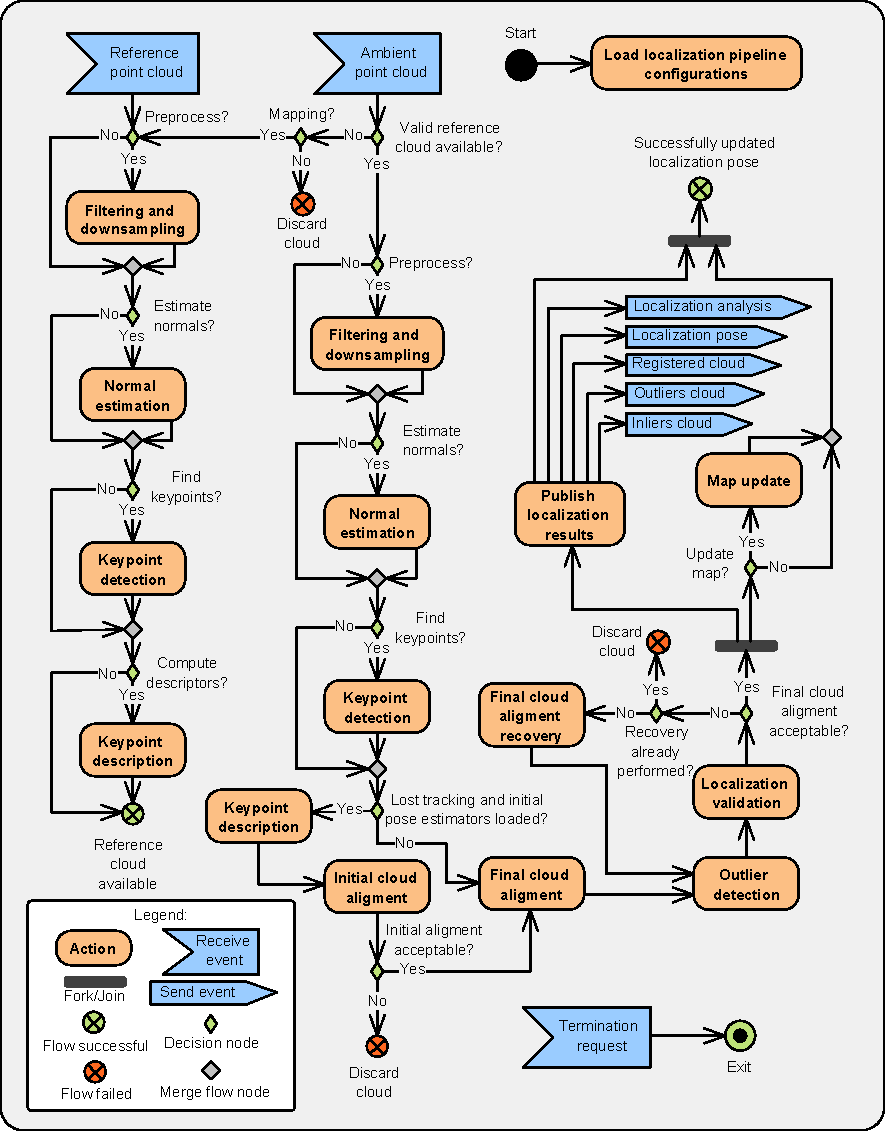
\includegraphics[width=0.45\textwidth]{localization-system/localization-system-overview}
	\caption{Localization system overview}
	\label{fig:localization-system_localization-system-overview}
\end{figure}


\subsection{Pipeline configuration}

The self-localization system was designed to allow fast reconfiguration\footnote{\url{https://github.com/carlosmccosta/dynamic_robot_localization/blob/hydro-devel/yaml/schema/drl_configs.yaml}} and parameterization through the use of yaml files and the \gls{ros} parameter server. This gives the possibility to quickly tune the localization system to the specific needs of a given mobile platform moving in a particular environment, in order to use the least amount of computational resources possible and without requiring any reprogramming or source code modification. Nevertheless, the system can use a generic configuration if hardware resources are not a concern.

In a typical configuration (following the \emph{Yes} paths of the activity diagram in \cref{fig:localization-system_localization-system-overview}), the first time the localization system is used, it receives a raw reference point cloud that is preprocessed and saved to long term memory along with its associated keypoints and keypoint descriptors. This allows a much faster startup the next time the localization system is initialized. After having a reference point cloud, the localization system will estimate the robot pose periodically by analyzing the ambient point cloud sensor data. This data can be preprocessed with several filters and can be associated with computed surface normals. The robot pose estimation is performed by applying a matrix transformation correction to the current robot pose and is based on the registration of the ambient point cloud with the know map. This registration can use a tracking algorithm configuration tuned for efficiency and a second configuration for tracking recovery purposes. These tracking algorithms require a initial pose estimation, and as such, if one isn't available, a third configuration can be employed to estimate the global position of the robot based on geometric features of the environment. The switch between these configuration is based on the analysis of the registered cloud metrics, such as outlier percentage, inliers root mean square error, inliers angular distribution and the registration corrections performed on the ambient point cloud. After successfully performing the robot pose estimation, the map can be updated by either integrating the full registered point cloud, its inliers or its outliers. Finally, like most \gls{ros} nodes, the localization system will stop its execution when it receives a termination signal request.

The next subsections explain in detail the architecture and algorithms used in each of the processing modules present in \cref{fig:localization-system_localization-system-overview}.


\subsubsection{Reference map}

The reference point cloud can be loaded from a \gls{cad} file, point cloud file or dynamically arrive trough a \gls{ros} topic as either a 3 \gls{dof} \emph{nav\_msgs::OccupancyGrid} or 6 \gls{dof} \emph{sensor\_msgs::PointCloud2}. This allows a localization supervisor to give only sections of a global map in order to use the least amount of memory and processing power (very large maps have deeper search structures, such as kd-trees, and should be avoided in order to improve the system efficiency).


\subsubsection{Point cloud assembly}

The self-localization system can use any sensor that provides point clouds, namely RGB-D / \gls{tof} cameras, \glspl{lidar} and stereo vision systems. Each of these types of sensors have very different operation rates and measurement accuracy. As such, the localization system allows the assembly of several ambient scans using a circular buffer in order to reduce the impact of sensor noise.

For \glspl{lidar}, the system provides a \emph{sensor\_msgs::LaserScan} assembler\footnote{\url{https://github.com/carlosmccosta/laserscan_to_pointcloud}} that converts laser measurements in polar coordinates into Cartesian coordinates and projects the points using spherical linear interpolation (in order to account for laser scan deformation that occurs when the robot is moving and rotating). It can merge scans from several lasers sensors and it will publish the final point cloud after assembling a given number of scans or periodically after a specified duration. These assembly configurations can be changed at runtime based on the robot velocity (for example, when the robots moves slower, more laser scans are assembled for each published point cloud) or through the use of the \gls{ros} dynamic reconfigure \gls{api}, which allows a navigation supervisor to control the rate at which the localization system operates.


\begin{figure}[hb]
	\centering
	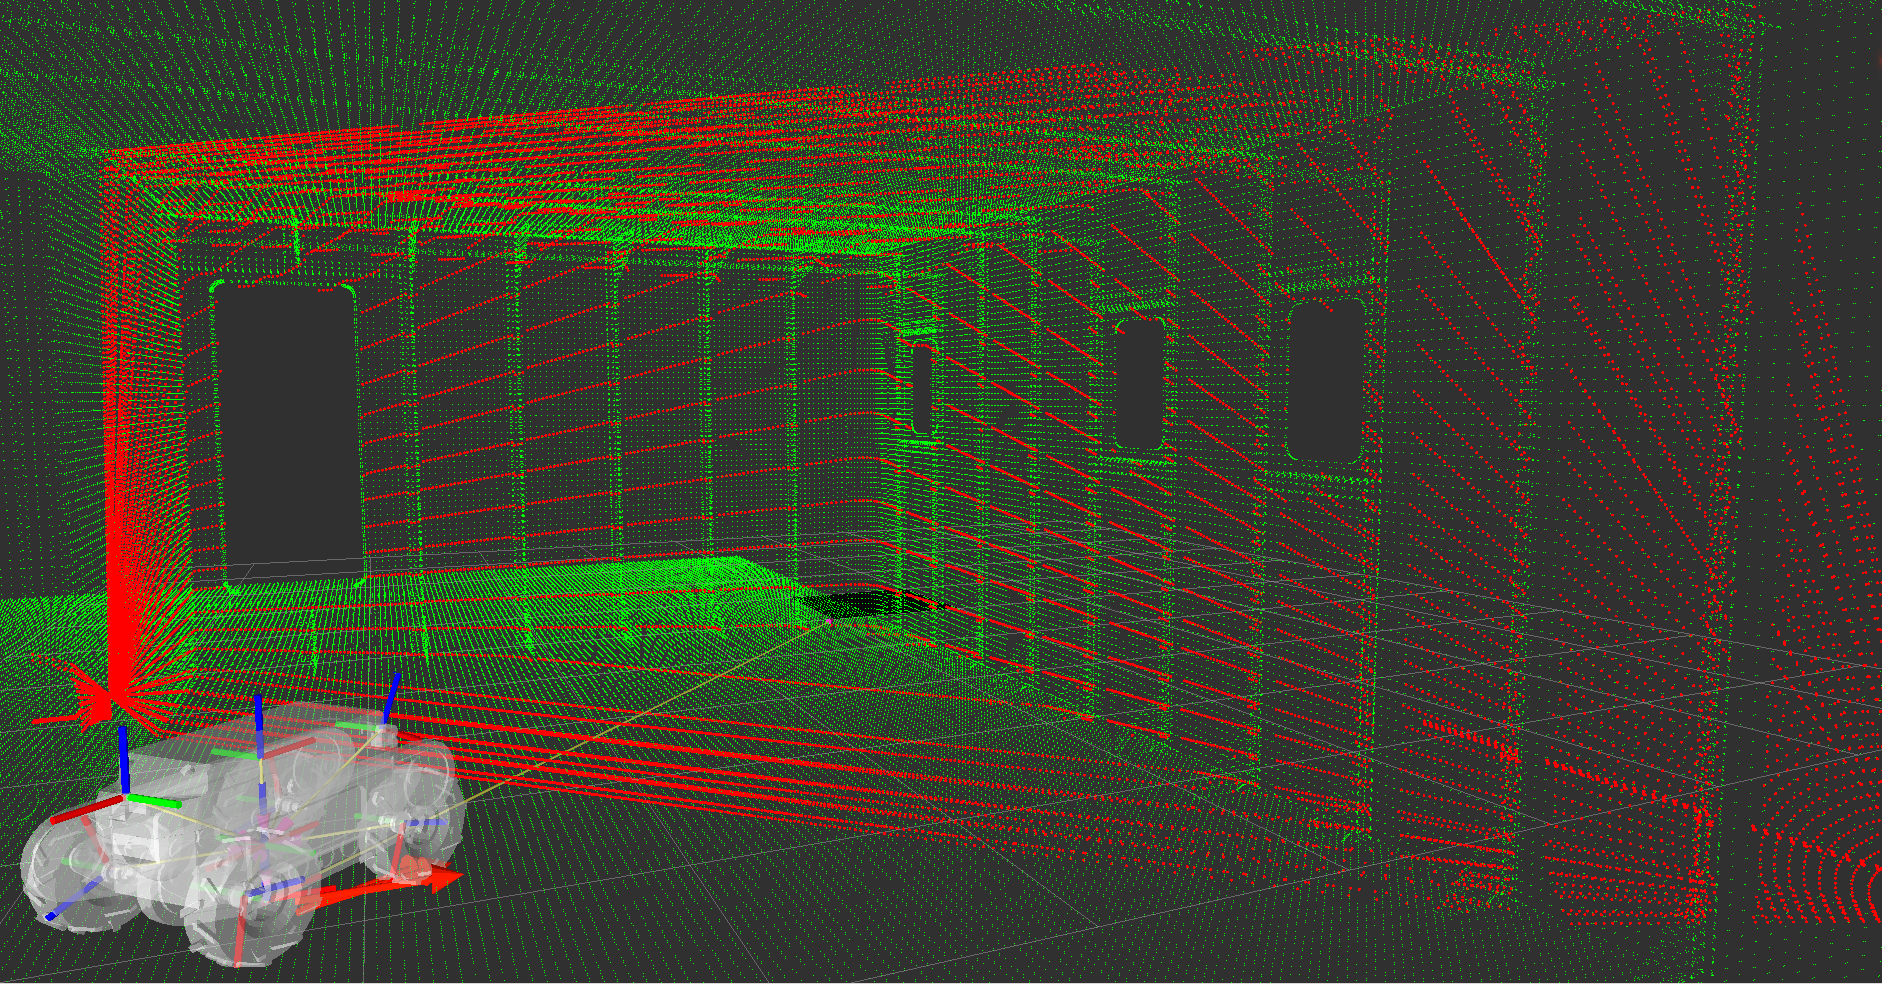
\includegraphics[width=0.42\textwidth]{localization-system/laser-assembly}
	\caption{Laser scans assembled with tilting platform (red points)}
	\label{fig:localization-system_section_laser_assembly}
\end{figure}


\subsubsection{Filtering and down sampling}

The time it takes to perform cloud registration increases considerable as the amount of points in the ambient point cloud and in the reference map becomes larger. As such, adjusting the level of detail of the point clouds by using voxel grids gives some control over the desired localization accuracy and the computational resources that will be required. This stage is also useful to mitigate the measurement errors of the depth sensors, since the centroid of a voxel that contains points from several scans will be closer to the real surface (if the voxels have dimensions slightly larger than the expected measurement errors).

The localization system allows the application of several preprocessing algorithms (algorithm type / configuration and execution order customizable). The next sections detail some of these methods that can be used to filter and downsample point clouds.


\paragraph{Voxel grid sampling}

A voxel grid is a uniform space partition technique that can be used to cluster points according to their Euclidean coordinates. It is a very effective method to control the level of detail of a point cloud because it gives the ability to specify the maximum number of points that a region of space should have.

The point cloud downsampling is achieved by replacing each voxel cluster with a single point. The selection of this point can be very fast if the voxel center is used, but computing the centroid of the cluster yields better results because it represents the underlying surface with more accuracy and it attenuates errors in the sensors measurements.


\paragraph{Random sampling}

Random sampling \cite{Vitter1984} is a fast downsampling method that randomly selects points from the input cloud until the specified number of samples is reached. This has the advantage of using real measures instead of downsampled approximations, but also means it is more sensible to sensor measurements noise. However, for outdoor environments or very complex scenes, using the real measurements can be preferable than using cluster centroids because the voxels may not have the necessary resolution or may have a prohibitive computational cost.


\paragraph{Covariance sampling}

Covariance sampling \cite{Gelfand} is a subsampling method that aims to create a stable downsampled point cloud to be registered with \gls{icp} algorithms. It incrementally builds the downsampled point cloud while trying to keep the 6 eigenvalues of the covariance matrix as close to each other as possible.

The resultant point cloud has the desired number of points and is stable enough to be matched with \gls{icp} point to plane algorithms.


\subsubsection{Outlier removal}

Some depth sensors can perform measurements with high accuracy, but they have some limitations that can lead to the creation of outliers \cite{Sotoodeh2006}.

One of those limitations can produce shadow points around objects boundaries. This is due to the fact that a portion of the laser beam may hit the object boundary and other part may hit other areas in the object background. And given that most laser range finders use a weighted sum of several beams, this can yield measurements that are not associated with any real object (outliers). Another issue is related to the angle in which the depth sensor sees the objects areas. If the incidence angle is very low, then it may be difficult to compute its distance and detect if the beam had ambient reflections. This can significant increase the measurements noise or even lead to the creation of outliers. Other common problem is associated with the material properties of the surfaces. For example, objects with very high or very low reflectance, such as metals or glass, can increase the measurements noise. Moreover depending on the combination of surface geometry, material and incidence angle, some objects may even be undetectable by depth sensors.

Given the negative effect that outliers have in surface normal computation and registration algorithms, they should be removed in a preprocessing stage. There are several approaches to perform outlier detection and removal \cite{YangZhang2010}, ranging from simple distance thresholds to more robust statistical analysis. The next sections present some of then that can be useful in a localization system.


\paragraph{Distance filter}

Given that depth sensors have a maximum recommended distance for their measurements, it is wise to remove points that are close or beyond this limit. Moreover, it may be useful to remove points that are too close to the sensor, because they may belong to the robot itself and not the environment.

This can be achieved by applying a minimum and maximum threshold to the distances returned by the depth sensor.


\paragraph{Passthrough filter}

A passthrough filter can select or remove points according to their properties.

For outlier removal, it can be used to select points that are within a given bounding box (useful when we already know what area of the environment we want to analyze) or remove points that don't have the appropriate intensity or color.


\paragraph{Radius outlier removal filter}

The radius outlier removal filter deletes points that don't have a minimum number of neighbors within a specified radius distance. It can be useful when the point density is known and is very effective in removing isolated points.


\paragraph{Statistical outlier removal filter}

The statistical outlier removal filter \cite{Rusu2010a} performs a global analysis of the distances between points and discards the ones that don't follow the global distance distribution.

It is a robust filter that adapts itself to the point cloud density and is very effective in removing shadow points. To do so, it computes the mean distance that each point has to a given number of neighbors and builds a global distance distribution. Then, assuming that the distribution is Gaussian, it discards the points that have a distance higher than a given threshold (that is a percentage of the standard deviation of the distance distribution).


\subsubsection{Surface and object reconstruction and resampling}\label{subsec:localization_system_surface-reconstruction-resampling}

Depending on the level of sensor noise and amount of outliers present in a given point cloud, it may be necessary to employ surface reconstruction techniques to fill gaps in sensor data or correct measurements errors.

The Moving least squares \cite{Alexa2003} is a surface reconstruction algorithm that uses higher order bivariate polynomials to fit surfaces to a given set of points. It can be used to fill possible gaps in sensor data, smooth the point cloud, refine surface normals and perform downsampling or upsampling.

Surface reconstruction can also be useful when the point cloud is built from several ambient scans with different origins and registered with some alignment errors. This allows to improve the points normals by using the surfaces computed by the moving least squares algorithm instead of using the point's neighbors.


\subsection{Normal estimation}

Most of feature detection, description and matching algorithms along with some registration methods rely on the point's surface normal and curvature. These algorithms analyze the neighborhood of a given point in order to compute the line / surface normal, and as such, the correct specification of what points should be included in the estimation is crucial to achieve accurate results. This depends on the environment geometry and the level of detail that is required, and is usually done by specifying a radius distance or by limiting the number of neighboring points to use.

The next sections describe some of the methods that are supported for 3/6 \gls{dof} sensor data.


\subsubsection{Line normal estimation}

Line normals give information about the spatial disposition and orientation of a given cluster of collinear points. They can be computed using \gls{ransac} methods \cite{Fischler1981} in which lines are fitted to the sensor data and their orientation corrected using the sensor's origin.


\subsubsection{Surface normal estimation}

Surface normals provide information about the orientation of the underlying geometry of a given point cluster. They can be computed using plane fitting methods or using more advanced techniques such as \gls{pca} \cite{Jolliffe2002} or the one presented in \cref{subsec:localization_system_surface-reconstruction-resampling}.


\subsection{Keypoint detection}

Aligning two point clouds with overlapping views of the environment requires the establishment of point correspondences. If both point clouds have similar sensor origins, these can be determined with nearest neighbor's searches and filtered with correspondence rejectors (using other point properties such as reflectance and color). But if they were acquired in two very different positions, then more advanced techniques must be employed.

One of those techniques uses histograms to describe the geometric properties of the environment around a given point. This allows points to be matched even if they have completely different Euclidean coordinates. Also, by using histograms and sampling techniques, these descriptors are much more robust against sensor noise and varying level of point density. However, these advantages come with a heavy computational cost, and as such, point descriptors should only be computed on the most descriptive areas of the environment.

Identifying these environment points is known as feature / keypoint detection \cite{Filipe2014}, and usually involves finding interesting points, such as corners and edges. Besides uniqueness, these points must also be repeatable. This means that the detection algorithms should be able to find the same points even if they are present in different point clouds with sensor noise and varying point density. This is of the utmost importance, because if the same keypoints are not identified on both clouds, then matching the point descriptors will likely fail.

Currently, the localization system can use the \gls{sift} \cite{Lowe2004} algorithm on the point's curvature or the \gls{iss3d} \cite{Zhong2009} keypoint detector on the point's normals.


\subsection{Keypoint description}

Describing a keypoint usually involves analyzing its neighboring points and computing a given metric or histogram that quantifies the neighbor's relative distribution, their normals angular relation, associated geometry or other metrics that are deemed useful. Several approaches were suggested over the years according to different recognition needs and they are the basis of feature matching algorithms used in the initial pose estimation.

The localization system can use most of the keypoint descriptors available in \gls{pcl}, namely the \gls{pfh} \cite{Rusu2008a}, the \gls{fpfh} \cite{Rusu2009}, the \gls{shot} \cite{Tombari2011}, the \gls{sc3d} \cite{Frome2004}, the \gls{usc} \cite{Tombari2010} and the \gls{esf} \cite{Wohlkinger2011}.


\subsection{Cloud registration}

Point cloud registration is the process of finding the transformation matrix (usually translation and rotation only) that when applied to a given ambient cloud will minimize an error metric (such as the mean square error of the ambient point cloud in relation to a given reference point cloud). Several approaches were suggested over the years and they can be categorized as point or feature cloud registration.


\subsubsection{Initial alignment with keypoints descriptor matching}\label{subsec:localization-system_feature-registration}

Feature registration is the process of matching keypoint descriptors in order to find an initial alignment between two point clouds. The proposed localization system uses a feature registration method similar to the \gls{sacia} algorithm presented in \cite{Rusu2009}. It uses a \gls{ransac} approach to select the best registration transformation after a given number of iterations. In each iteration a subsample of randomly selected descriptors from the ambient cloud is retrieved. Then for each of these descriptors, $k$ best matching descriptors in the reference point cloud are searched (using a kd-tree) and one of them is chosen randomly (this improves robustness against noise in the sensor data and changes in the environment that are not yet integrated into the map). Later after having filtered these correspondences between ambient and reference descriptors, the registration matrix is computed. If this registration matrix results in a point cloud overlap that has a minimum of inliers percentage (a point in the ambient cloud is an inlier if it has a point in the reference cloud closer than a given distance), then it is considered an acceptable initial pose and is saved (to allow a localization supervisor to analyze the distribution of the acceptable initial poses). In the end of all iterations, the best initial pose (if found) is refined with a point cloud registration algorithm.


\subsubsection{Final alignment with point cloud error minimization}

Point cloud registration algorithms such as \gls{icp} \cite{Besl1992} (with its several known variations \cite{Rusinkiewicz2001,Pomerleau2013} like \gls{icp} point-to-point, \gls{icp} point-to-point non-linear, \gls{icp} point-to-plane and generalized \gls{icp} \cite{Segal2009}) and the \gls{ndt} \cite{Magnusson2009} are among the most popular algorithms to register point clouds. They can achieve very accurate cloud registration but they require an approximate initial pose for the registration to successfully converge to a correct solution (otherwise they may achieve only partial cloud overlap or even fail to converge to a valid solution).


\subsection{Outlier detection}

Detecting which points of the environment are not part of the reference point cloud can be very useful to evaluate the quality of point cloud registration as well as to analyze the presence of previously unknown objects. It's computation splits the ambient cloud into two point sets. One containing inliers (points correctly registered and present in the reference point cloud) and the other having the outliers (points that are either incorrectly registered or not present in the reference cloud).

A given ambient point can be classified as outlier if the corresponding closest point in the reference cloud is farther way than a given distance threshold. These calculation can be done efficiently by using the reference point cloud kd-tree. In \cref{fig:localization-system_outlier-detection} is an example of a ambient point cloud retrieved with a tilting laser and registered with an indoor map (yellow points). After registration, the ambient point cloud was split into inliers (red points) and outliers (blue points).


\begin{figure}
	\centering
	\begin{subfigure}[h]{0.45\textwidth}
		\centering
		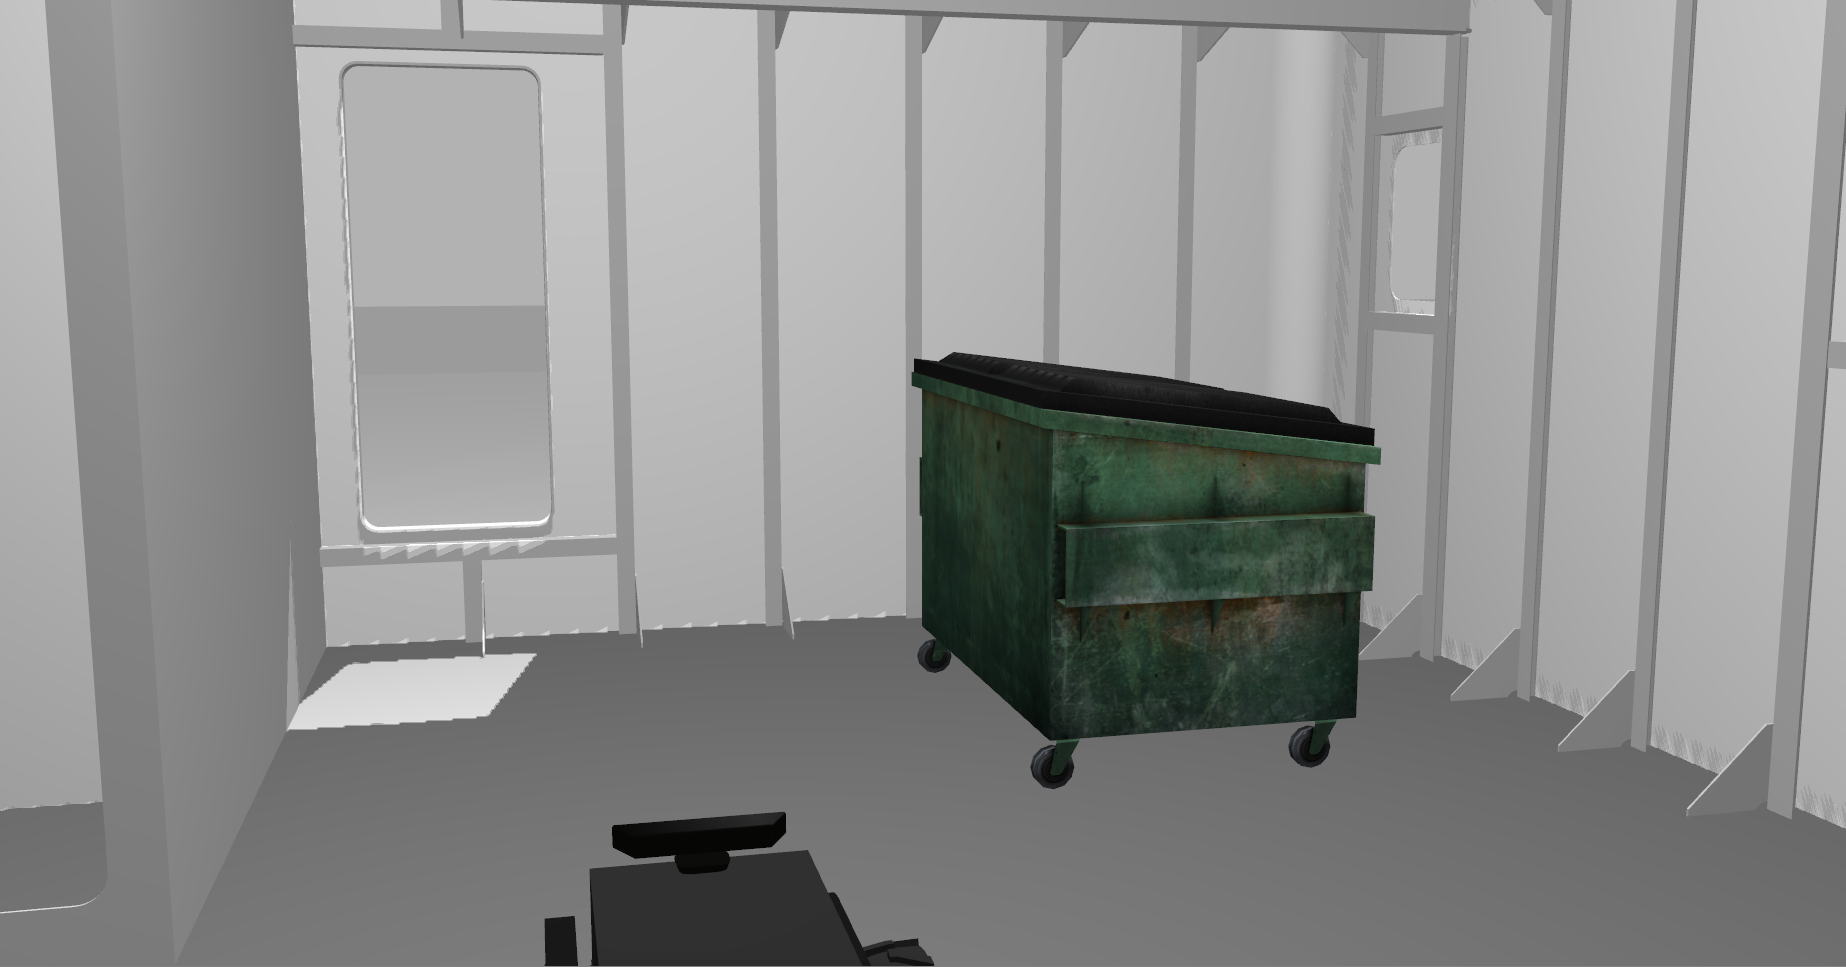
\includegraphics[width=\textwidth]{localization-system/outlier-detection-gazebo}
		\caption{Gazebo overview}
	\end{subfigure}
	\begin{subfigure}[h]{0.45\textwidth}
		\centering
		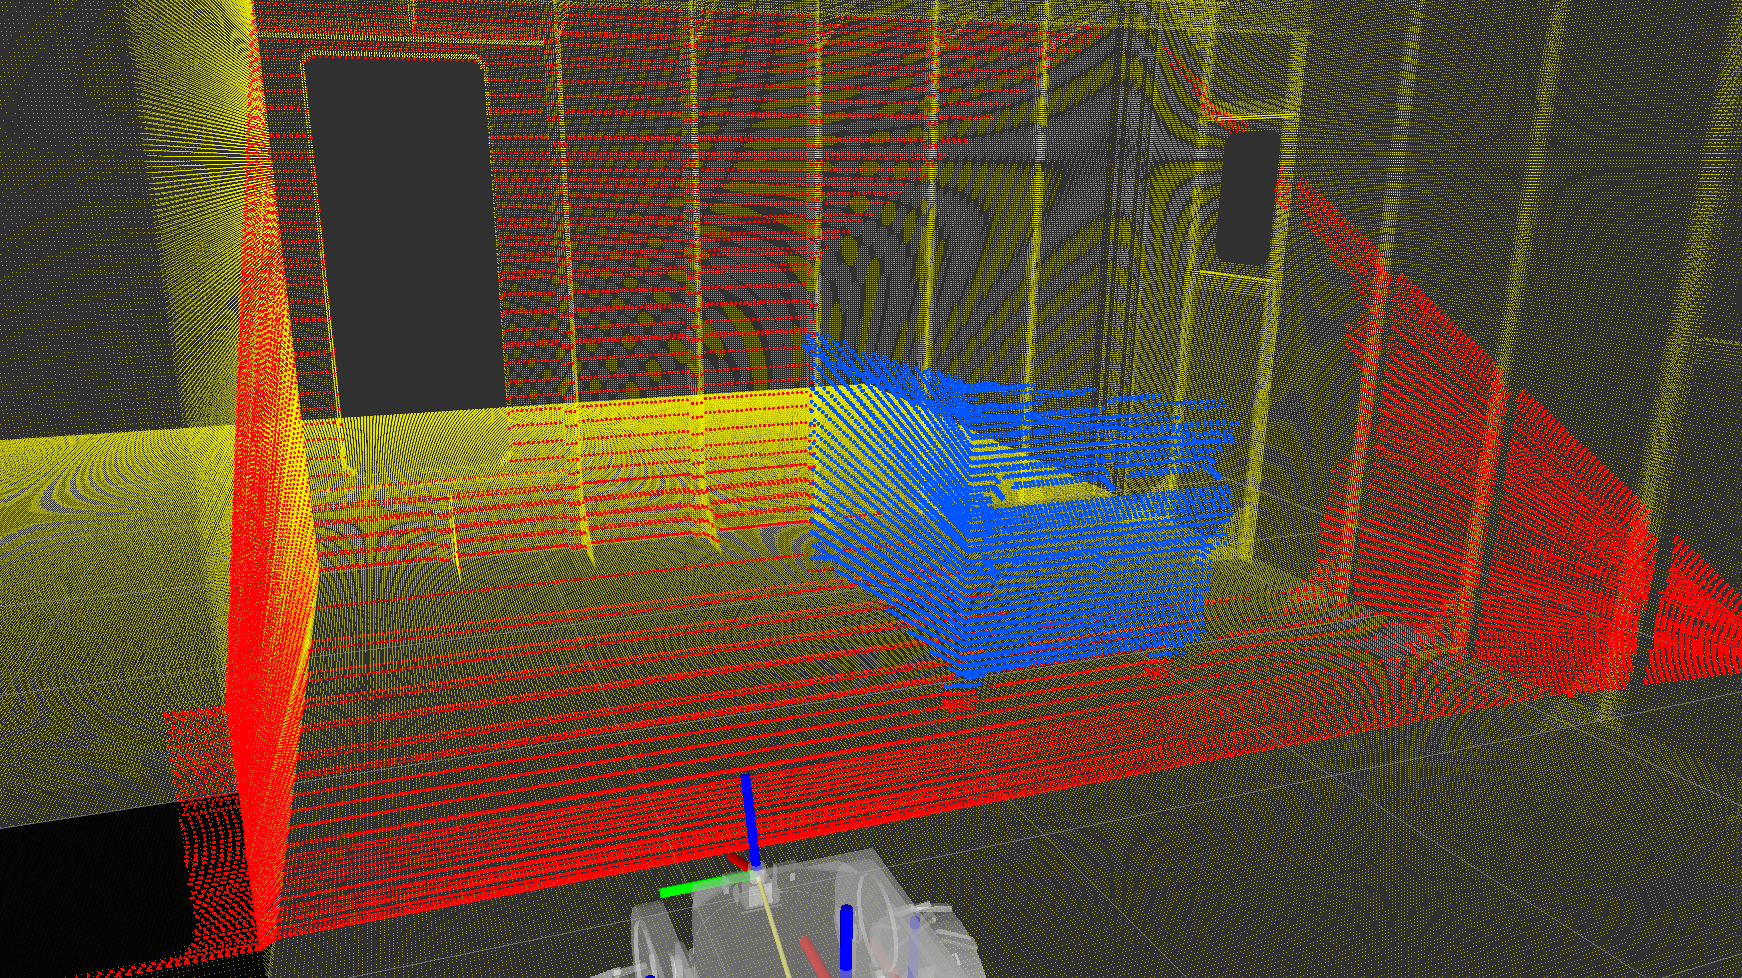
\includegraphics[width=\textwidth]{localization-system/outlier-detection}
		\caption{RViz overview}
	\end{subfigure}\hfill
	\caption{Point cloud registration with outlier detection}
	\label{fig:localization-system_outlier-detection}
\end{figure}


\subsection{Localization validation}

After a point cloud is registered by the localization system, several metrics are calculated in order to evaluate if a valid pose can be retrieved using the registration matrix.

The first computed metrics are the percentage of inliers and the \gls{rmse} of these inliers. If a minimum number of points was registered and the inlier percentage and root mean square error are acceptable, then the registration is considered successful. However, these registered points can be agglomerated in a small area and may not be representative of the robot location. As such, a second metric is computed that takes into account the angular distribution of these inliers. This metric gives a measurement of how reliable is this registration and is based on the fact that there is high confidence in a given pose estimation when there are correctly registered points all around the robot.

The last metrics are the corrections that the registration matrix introduced. Given that the localization system will be in tracking mode most of the time, it is possible to define how far a new pose can be in relation to the previous accepted location and discard new poses that exceed a given threshold. This is useful to discard pose corrections that are very unlikely to happen, such as the robot moving half a meter between poses when it is expected to move only at 30 cm/s. These situations can happen when there is a sudden decrease in the field of view (that can occur due to sensor occlusion or malfunction) or when large unknown objects very similar to sections of the map appear into the field of view of the robot.

If all these metrics are within acceptable thresholds, then the robot pose can be computed by applying the matrix correction to the initial pose associated with the ambient sensor data. If any of these metrics are not acceptable, then the system can be configured to simply discard this pose estimation and try to estimate the pose in the next sensor data update or it can apply a tracking recovery attempt with a different registration algorithm (or the same algorithm with different parameters). If several consecutive pose estimations are discarded, the system can have a second level of recovery that can be configured to use the initial pose estimation algorithms in order to finally estimate the robot pose and reset the tracking state.


\section{Dynamic map update}

After performing a successful pose estimation, the localization system can update the localization map by either integrating only the unknown objects or the full registered point cloud (it can also be used in conjunction with OctoMap \cite{Hornung2013} to perform probabilistic map updates). Integrating only the unknown objects is the recommended approach when there is a known map and the environment is expected to change gradually. This is also more efficient as only the points that need to be integrated are processed and ray traced in OctoMap. On the other hand, integrating the full registered cloud can be desirable if the map of the environment is very incomplete, very outdated or expected to change considerably during the operation of the robot.

\section{Testing configurations}\label{sec:testing-configurations}

This section presents several test scenarios that were devised to evaluate the implemented localization system. They aim to test the accuracy and robustness of the implementation under different environmental conditions and hardware configurations.


\subsection{Testing platforms}

The localization system was tested on laser sensor data retrieved from three different mobile robot platforms and executed on the same computer in order to allow a direct comparison of computation time. This computer was a Clevo P370EM3 laptop (with a Intel Core i7 3630QM CPU at 2.4GHz, 16 GB of RAM DDR3, NVidia GTX680M graphics card and a Samsung 840 Pro SSD) and it was running Ubuntu 12.04 along with \gls{ros} Hydro, \gls{pcl} 1.7 and Gazebo 1.9.

The sensor data was recorded into rosbags, and is publicly available at\footnote{\url{https://github.com/carlosmccosta/dynamic_robot_localization_tests}} along with all the detailed results, configurations and experiments videos, in order to allow future comparisons with other localization systems. The hardware specifications of the \glspl{lidar} used is presented in \Cref{tab:localization-system-evaluation_laser-hardware-specifications} and the laser points after downsampling and registration can be seen on the movement paths figures as green dots (inliers) and red dots (outliers).


\subsubsection{Jarvis platform}

The Jarvis platform is an autonomous ground vehicle equipped with a SICK NAV 350 laser for self-localization (mounted about 2 meters from the floor) and a SICK S3000 laser for collision avoidance (mounted about 0.20 meters from the floor). It uses a tricycle locomotion system with two back wheels and a steerable wheel at the front. In \Cref{fig:localization-system-evaluation_jarvis} the robot is performing a delivery task with the package on top of a moving support. The 3 \gls{dof} ground truth was provided by the SICK NAV350 system and relied on 6 laser reflectors (with 9 cm of diameter) to perform the pose estimations (it is certified for robot docking operations with precision up to 4 millimeters).


\subsubsection{Pioneer 3-DX platform}

The Pioneer 3-DX shown in \Cref{fig:localization-system-evaluation_pioneer} is a small lightweight robot equipped with a SICK LMS-200 laser (mounted about 48 cm from the floor) and a Kinect (mounted about 78 cm from the floor). It uses a two-wheel two-motor differential drive locomotion system and can reach a linear speed of 1.2 m/s and angular velocity of 300º/s. The 3 \gls{dof} ground truth was provided by 8 Raptor-E cameras \footnote{\url{http://www.motionanalysis.com/html/movement/raptore.html}} and according to \cite{Sturm2012} it had less than 1 cm in translation error and less than 0.5 degrees in rotation error.

\begin{figure}[H]
	\centering
	\begin{minipage}[hb]{0.24\textwidth}
		\centering
		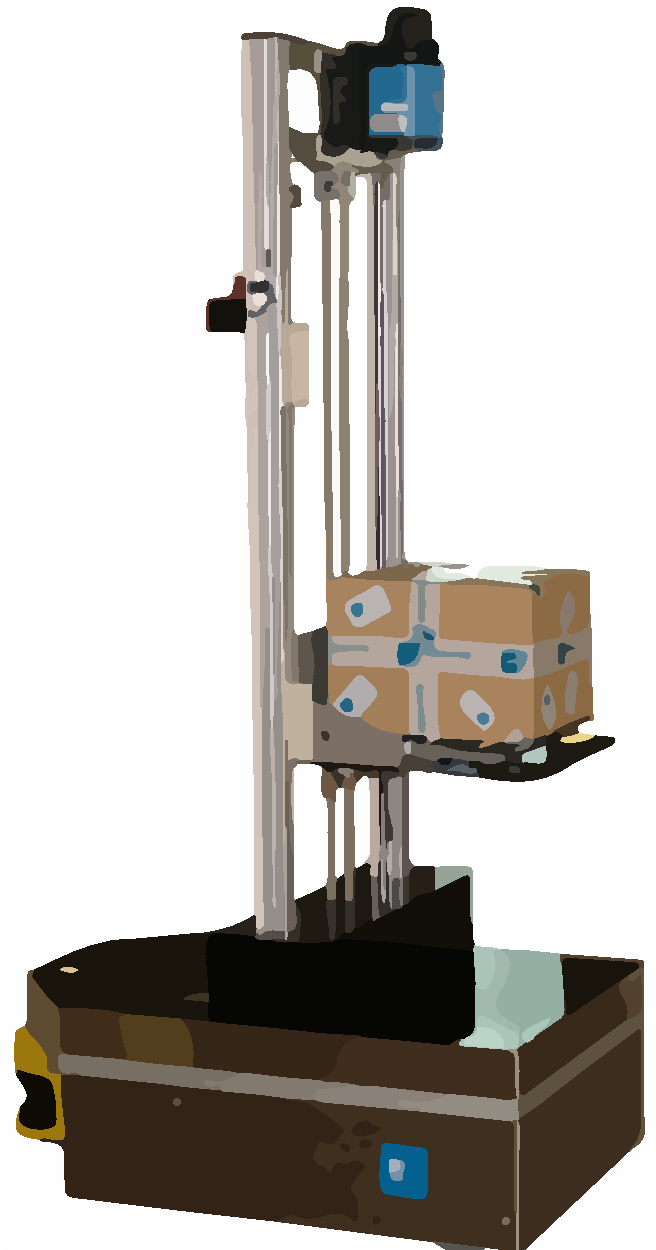
\includegraphics[width=0.8\textwidth]{localization-system-evaluation/testing-platforms/jarvis}
		\caption{Jarvis testing platform}
		\label{fig:localization-system-evaluation_jarvis}
	\end{minipage}\hfill
	\begin{minipage}[hb]{0.24\textwidth}
		\centering
		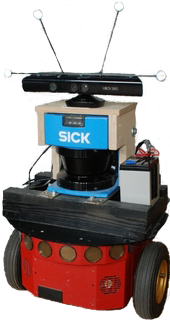
\includegraphics[width=0.7\textwidth]{localization-system-evaluation/testing-platforms/pioneer-3dx}
		\caption{Pioneer 3-DX testing platform \cite{Sturm2012}}
		\label{fig:localization-system-evaluation_pioneer}
	\end{minipage}
\end{figure}


\subsubsection{Guardian platform}

The Guardian platform is an autonomous mobile manipulator equipped with a Hokuyo URG-04LX laser in the front and a Hokuyo URG-04LX\_UG01 laser in the back (both mounted about 0.37 meters from the ground). The front laser had a tilting platform which allows 3D mapping of the environment. The arm is a SCHUNK Powerball LWA 4P and in \Cref{fig:localization-system-evaluation_guardian} it is attached to a stud welding machine (in simulation it is attached to a video projector). It uses a differential drive locomotion system and can be moved with wheels or with tracks. This platform didn't have a certified ground truth and as such, the results could not be quantified with an external localization system (the results performed with the Gazebo simulator will be presented instead - robot model shown in \Cref{fig:localization-system-evaluation_guardian_gazebo}).

\begin{figure}[H]
	\centering
	\begin{minipage}[hb]{0.24\textwidth}
		\centering
		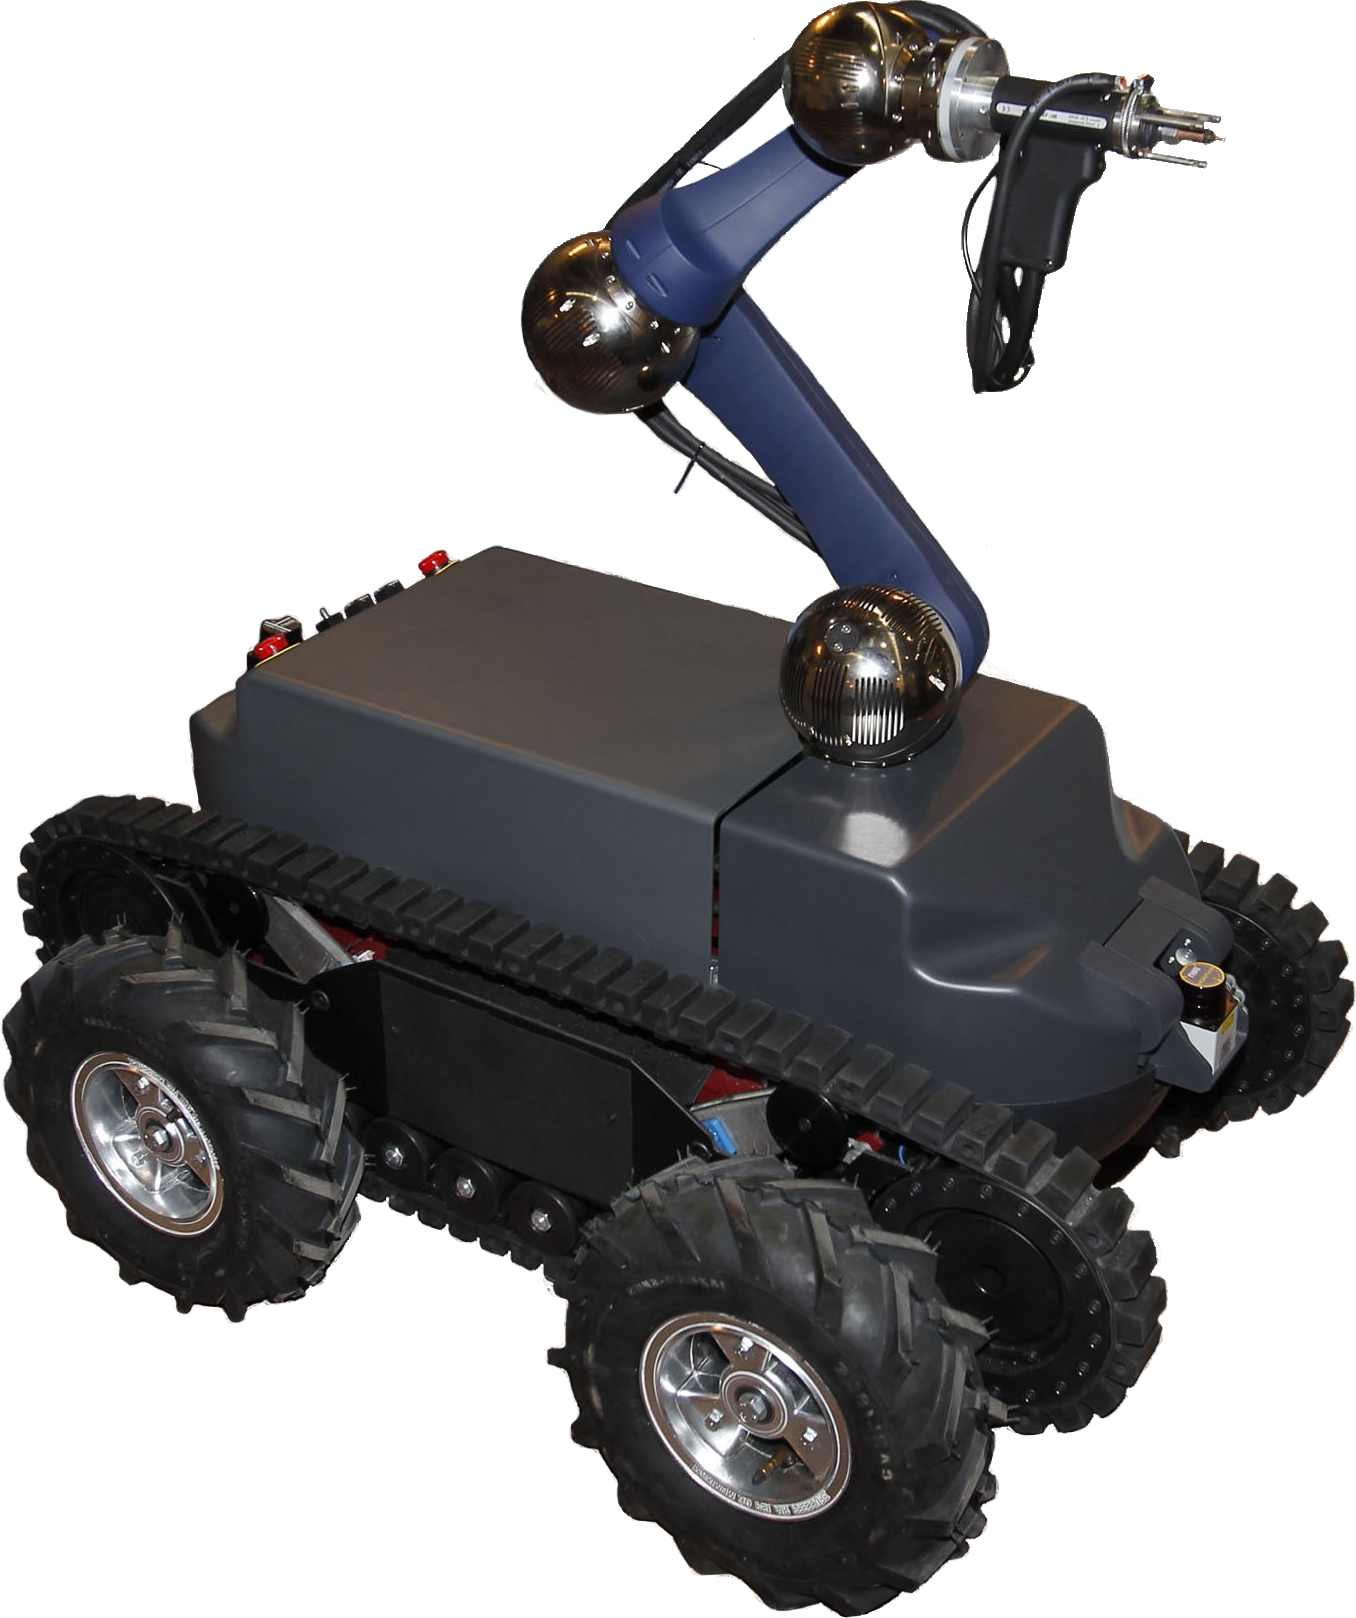
\includegraphics[width=0.84\textwidth]{localization-system-evaluation/testing-platforms/guardian}
		\caption{Guardian testing platform}
		\label{fig:localization-system-evaluation_guardian}
	\end{minipage}\hfill
	\begin{minipage}[hb]{0.24\textwidth}
		\centering
		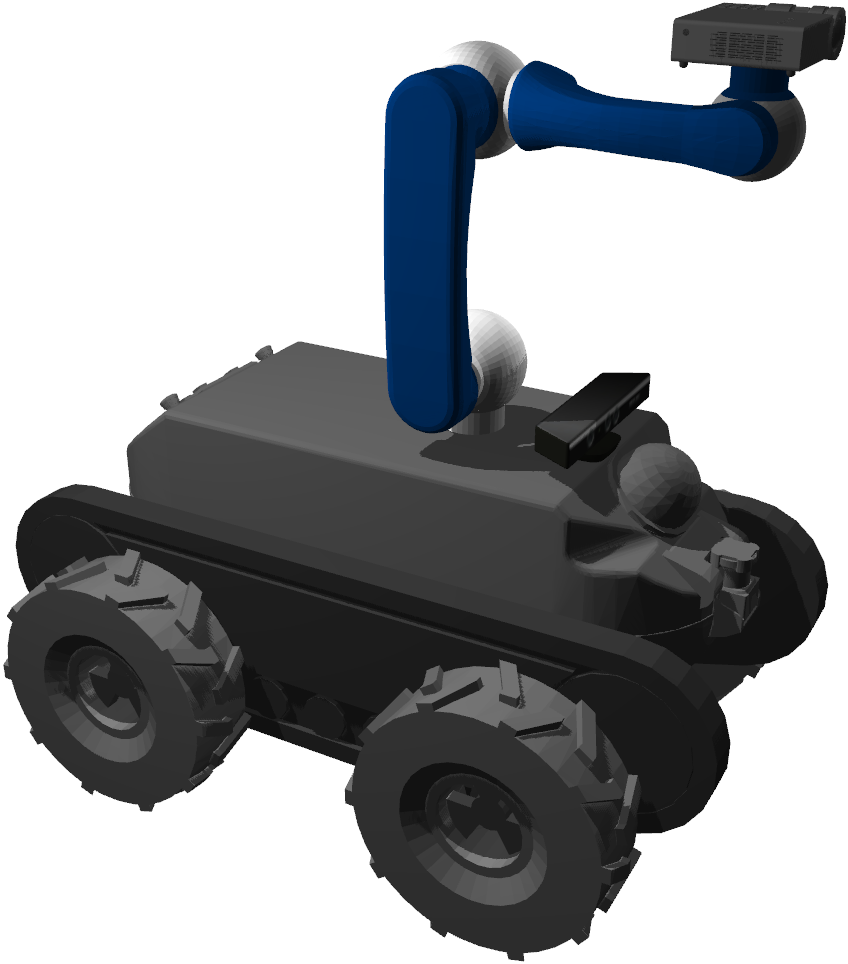
\includegraphics[width=0.84\textwidth]{localization-system-evaluation/testing-platforms/guardian-gazebo}
		\caption{Guardian Gazebo simulation}
		\label{fig:localization-system-evaluation_guardian_gazebo}
	\end{minipage}
\end{figure}


\begin{table*}[t]
	\caption{\glsentryplural{lidar} hardware specifications}
	\tabulinesep = 0.8ex
	\centering
	\small
	\begin{tabu} { X[2.5,m,c] | X[m,c] X[m,c] X[m,c] X[m,c] X[m,c] }
		\rowfont{\bfseries\itshape\small} Laser model & Range (meters) & Field of view (degrees) & Scanning frequency (Hz) & Angular resolution (degrees) & Statistical error (millimeters) \\
		\hline
		{\small SICK NAV350} 			& [0.5..250] 	& 360 	& 8 	& 0.25 	& 15 	\\
		{\small SICK S3000} 			& [0.1..49] 	& 190 	& 8 	& 0.25 	& 150 	\\
		{\small SICK LMS200} 			& [0.1..80] 	& 180 	& 10 	& 1.0 	& 35 	\\
		{\small Hokuyo URG-04LX} 		& [0.06..4.095] & 240 	& 10 	& 0.36 	& 10 	\\
		{\small Hokuyo URG-04LX\_UG01} 	& [0.02..4] 	& 240 	& 10 	& 0.36 	& 30 	\\
	\end{tabu}
	\label{tab:localization-system-evaluation_laser-hardware-specifications}
\end{table*}



\subsection{Testing environments}

The localization system was tested in different environments and used the Jarvis platform in a large room with a RoboCup field, the Pioneer 3-DX in a large industrial hall, the Guardian platform in a simulated indoor environment and a Kinect in a flying arena.


\subsubsection{Jarvis in RoboCup field}

The RoboCup field (shown in \Cref{fig:localization-system-evaluation_jarvis-tests-environment}) occupies half of a large room (with 20.5 meters of length and 7.7 meters of depth). It has two doors, several small windows and two large glass openings into the hallway. Several tests were performed with the robot at speeds ranging from 5 cm/s to 50 cm/s in this environment and up to 2 m/s using the Stage simulator\footnote{\url{http://rtv.github.io/Stage/}}. These tests were performed with two different movement paths. The first is a simple rounded path that aimed to test the robot in the region of space that had better ground truth (due to its position in relation to the laser reflectors). The second path was more complex and contained several sub paths with different velocities and shapes (it was intended to evaluate the localization system with typical movements that mobile manipulators require, such as moving forward and backwards with or without angular velocity and stopping at the desired destination).


\begin{figure}[H]
	\centering
	\begin{subfigure}[ht]{0.31\textwidth}
		\centering
		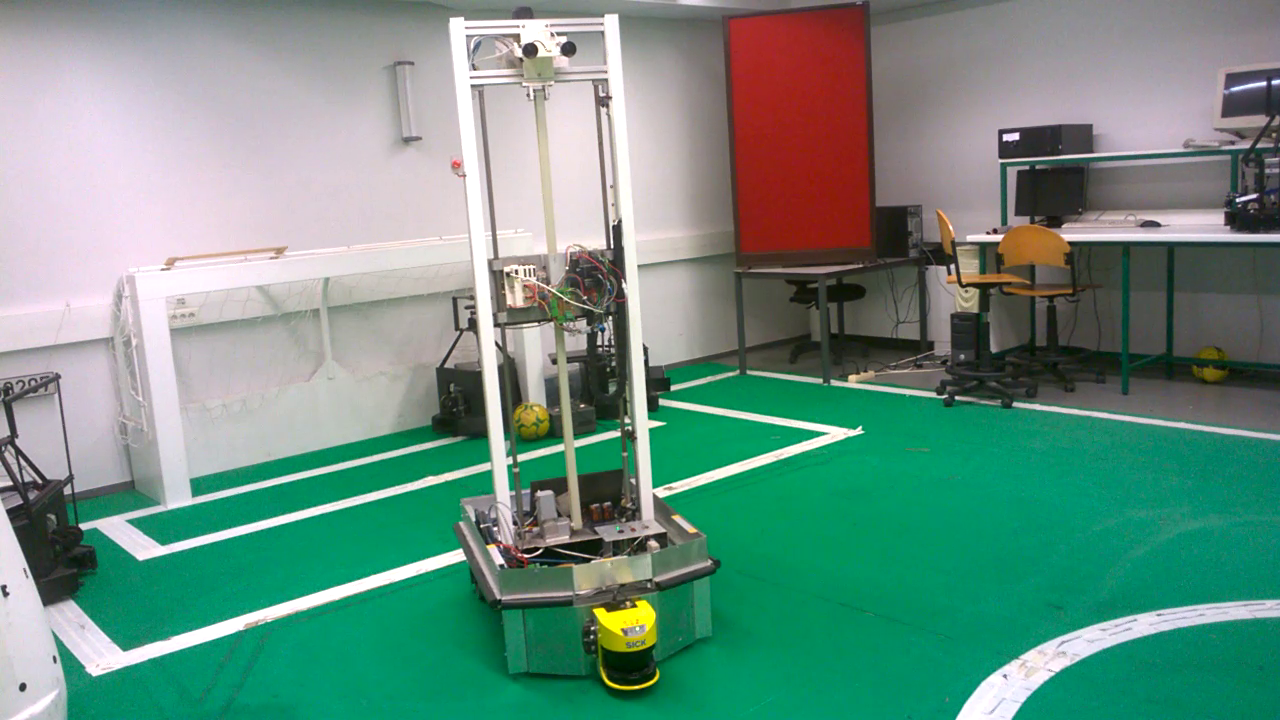
\includegraphics[width=\textwidth]{localization-system-evaluation/testing-environments/jarvis-environment-front-left}
	\end{subfigure}
	\begin{subfigure}[ht]{0.31\textwidth}
		\centering
		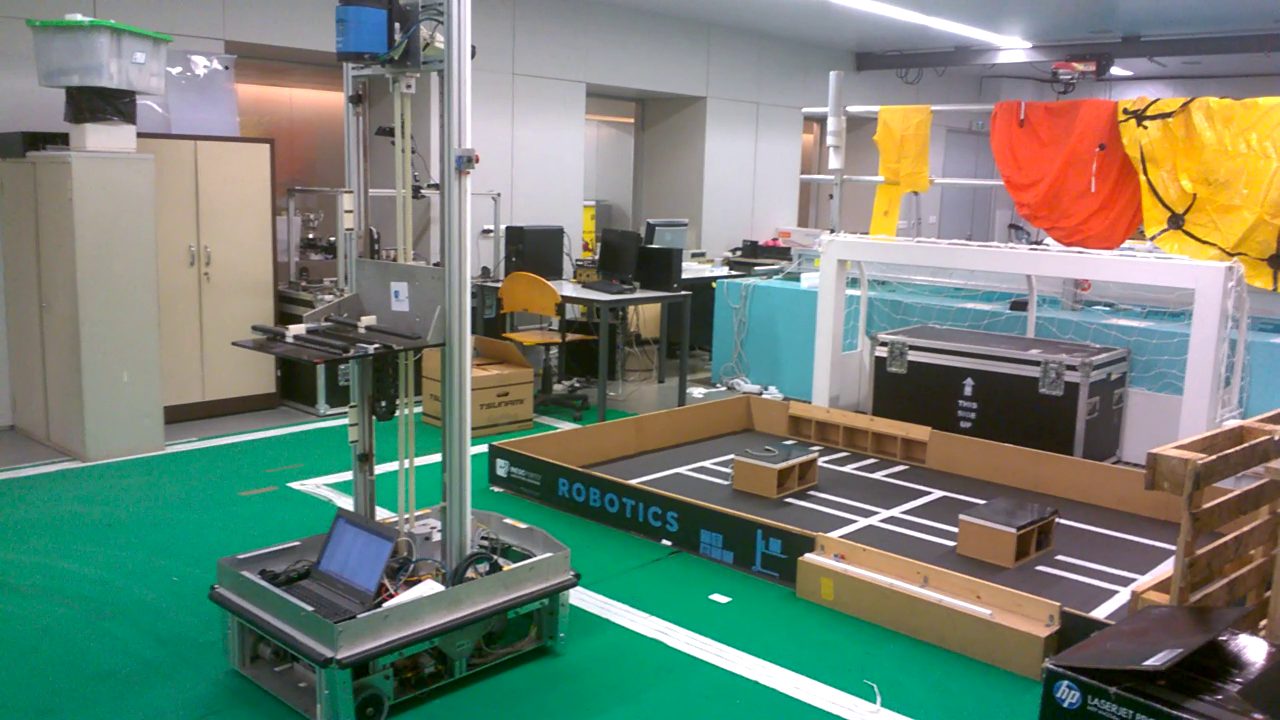
\includegraphics[width=\textwidth]{localization-system-evaluation/testing-environments/jarvis-environment-front-right}
	\end{subfigure}
	\caption{Jarvis testing environment}
	\label{fig:localization-system-evaluation_jarvis-tests-environment}
\end{figure}


\subsubsection{Guardian in structured environment}

The structured environment simulated in Gazebo is a large room with 12.4 meters of length and 8.4 meters of depth. It has 4 doors, several small windows and the walls have small ledges at regular intervals.

Given that the Guardian mobile manipulator is expected to work on the walls of this environment, several tests were devised with a path following the lower and right wall of the environment. The first test was done in a static environment clear of unknown objects and was meant to evaluate the best precision that the localization system could achieve. The second test was done in a cluttered environment and was designed to test the robustness of the localization system against static unknown objects, that were placed in the middle of the environment and close to the walls (to block sensor data from reaching known positions and analyze the robustness of matching unknown points that are close to known areas). The last test added a moving car to the scene and aimed to assess the impact of dynamic objects on the point cloud registration algorithms.


\begin{figure}[H]
	\centering
	\begin{subfigure}[ht]{0.25\textwidth}
		\centering
		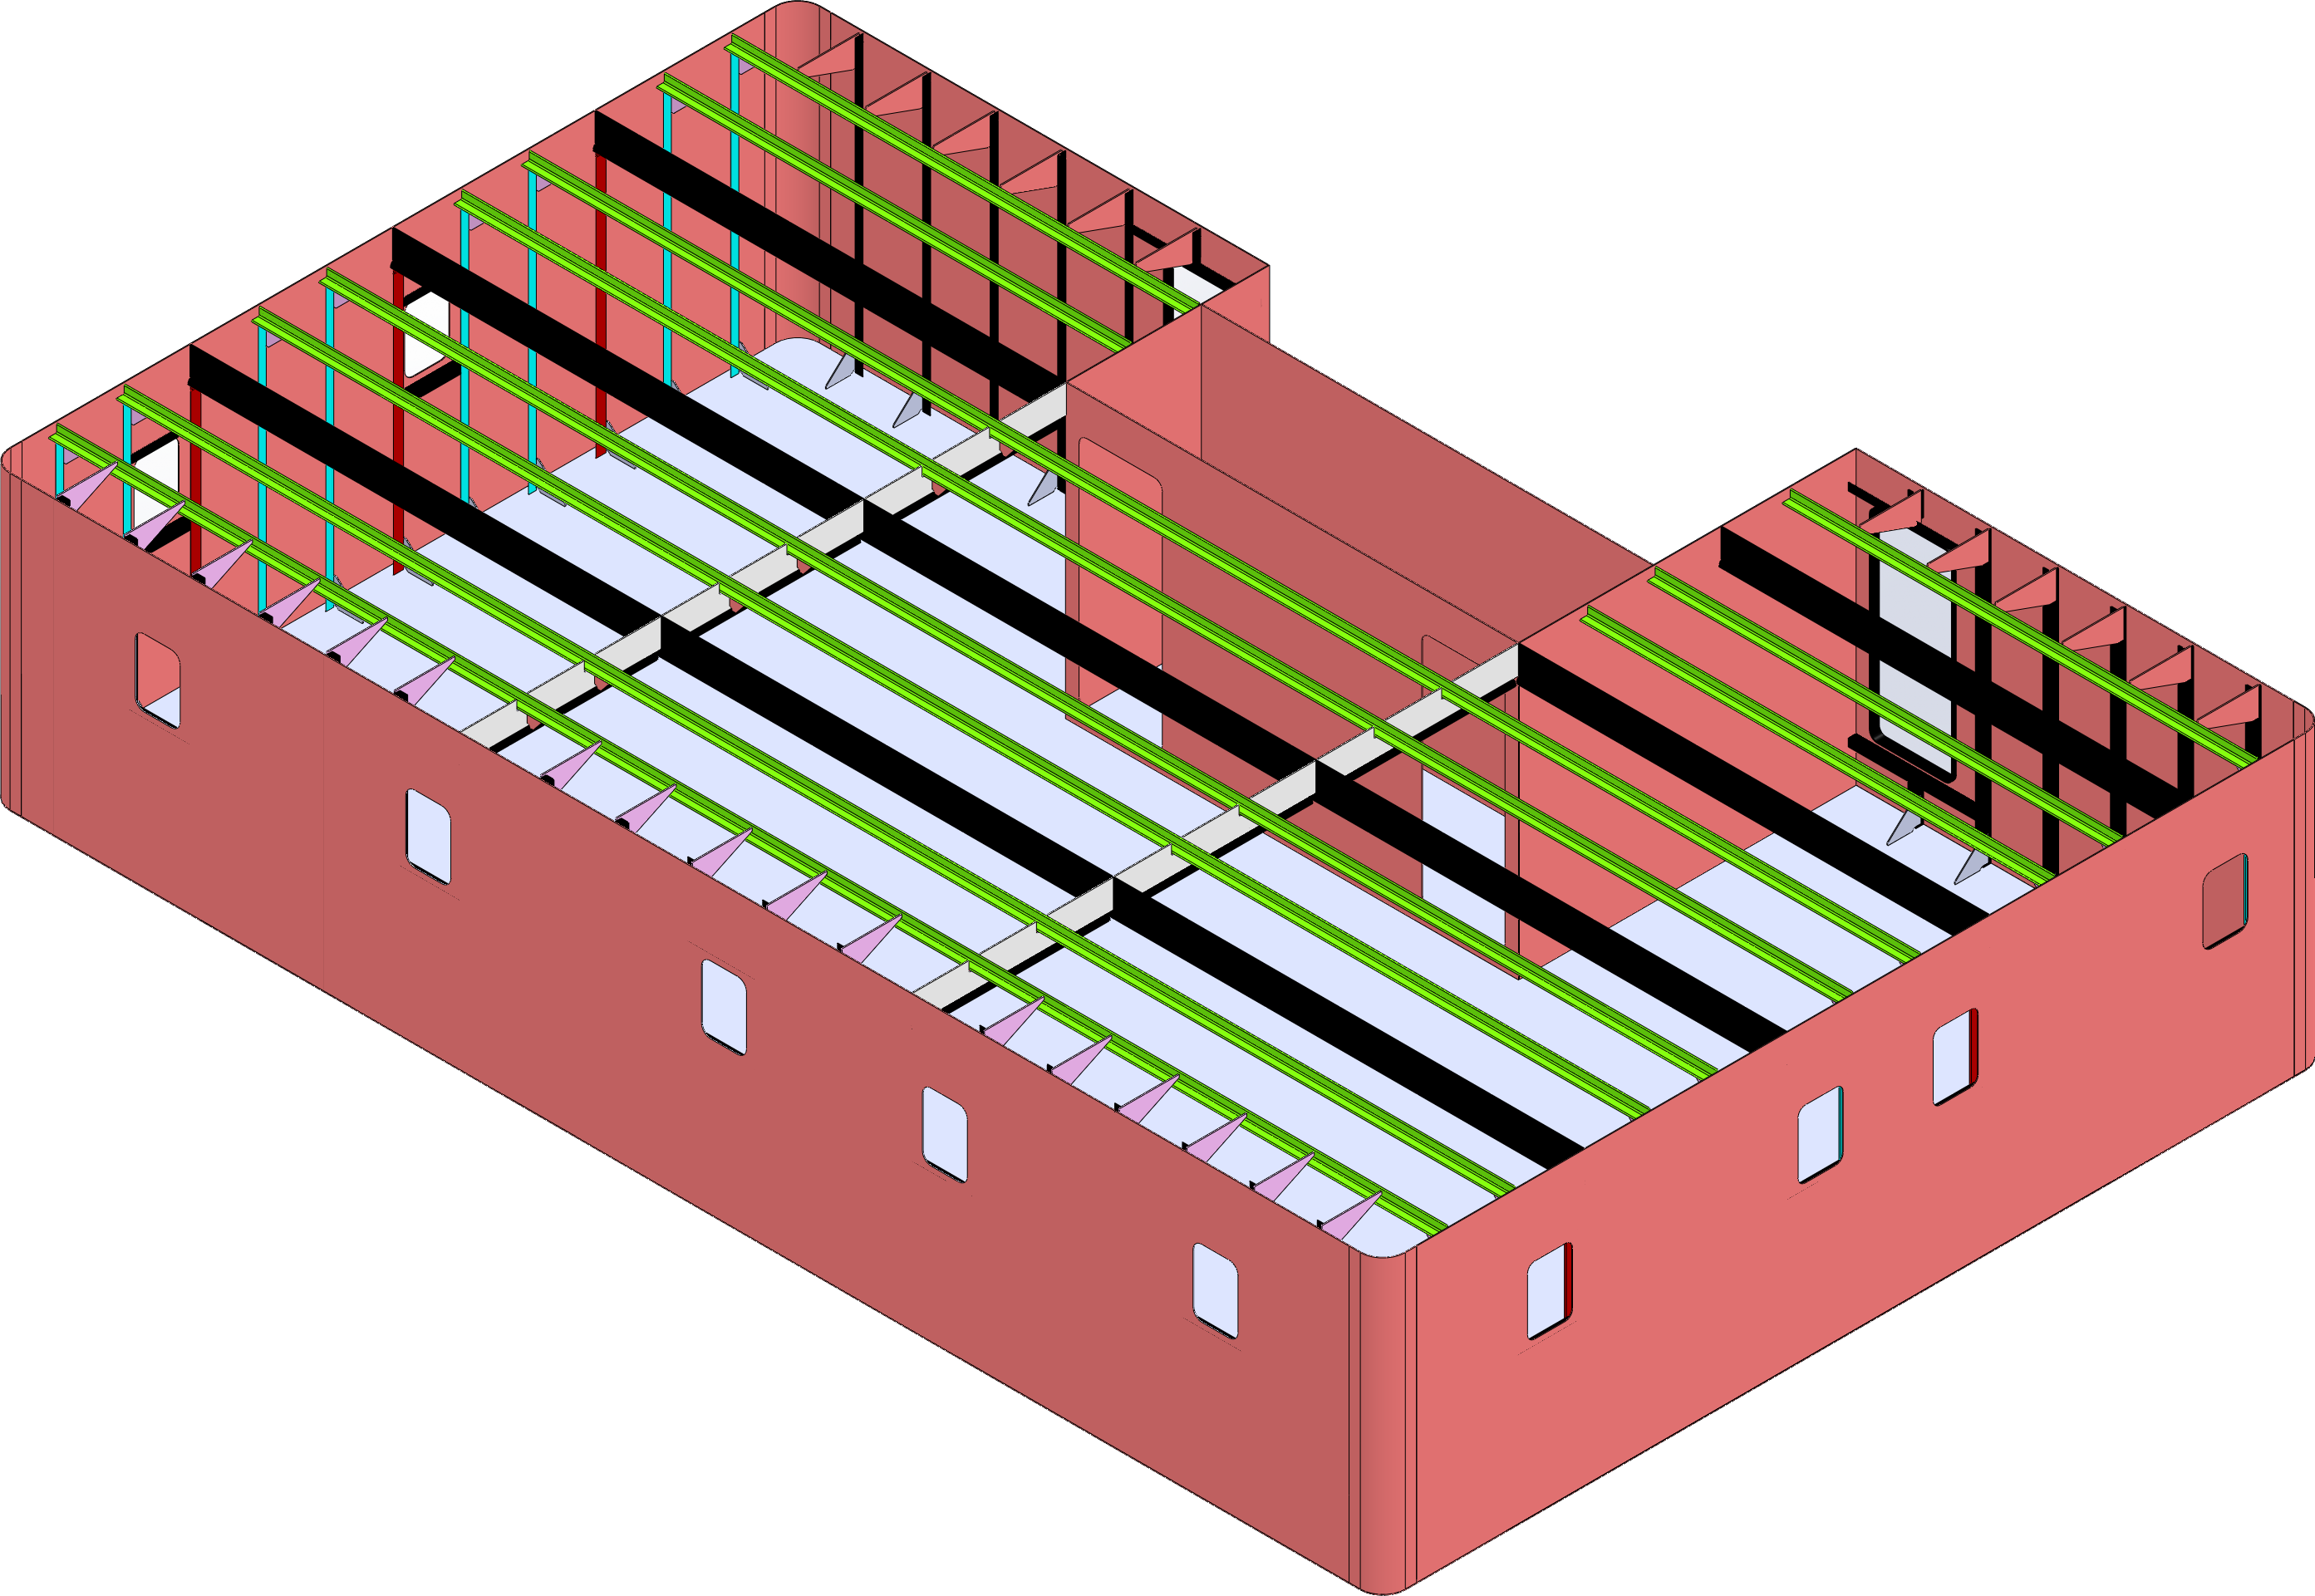
\includegraphics[width=\textwidth]{localization-system-evaluation/testing-environments/guardian-environment-corner}
	\end{subfigure}
	\begin{subfigure}[ht]{0.25\textwidth}
		\centering
		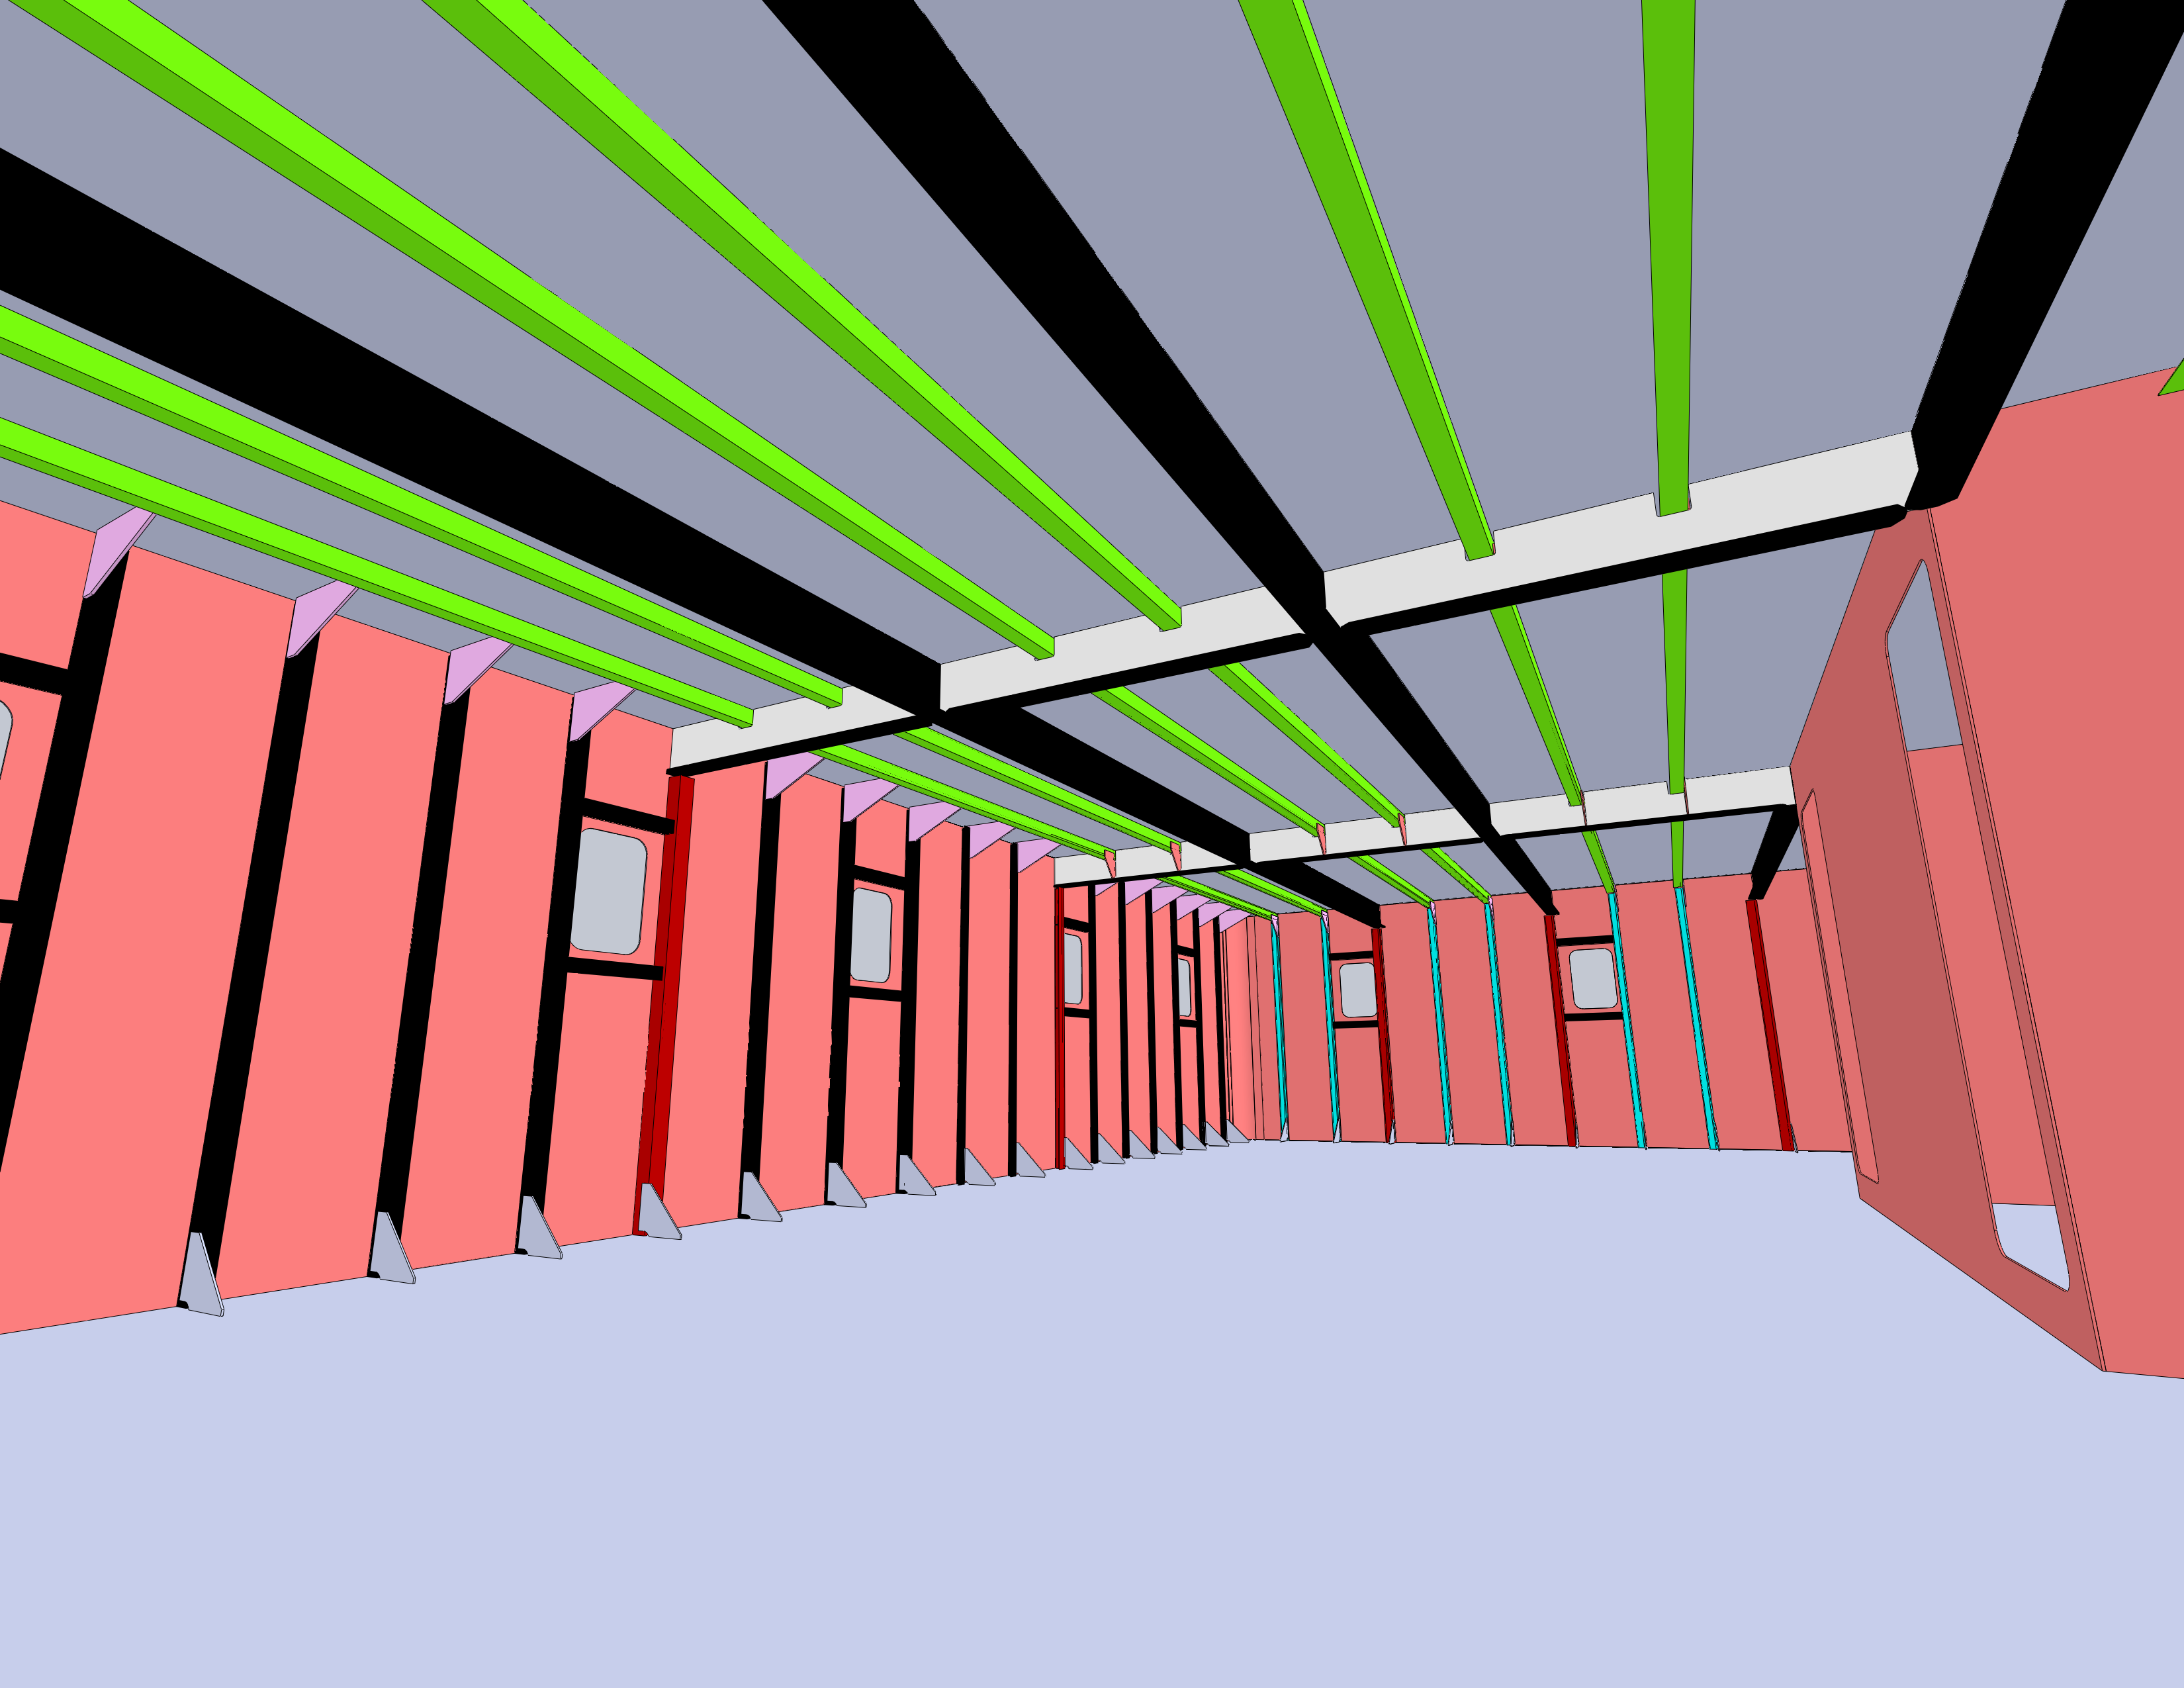
\includegraphics[width=\textwidth]{localization-system-evaluation/testing-environments/guardian-environment-inside}
	\end{subfigure}
	\caption{Guardian testing environment}
	\label{fig:localization-system-evaluation_guardian-tests-environment}
\end{figure}

\begin{figure}[H]
	\centering
	\begin{subfigure}[ht]{0.4\textwidth}
		\centering
		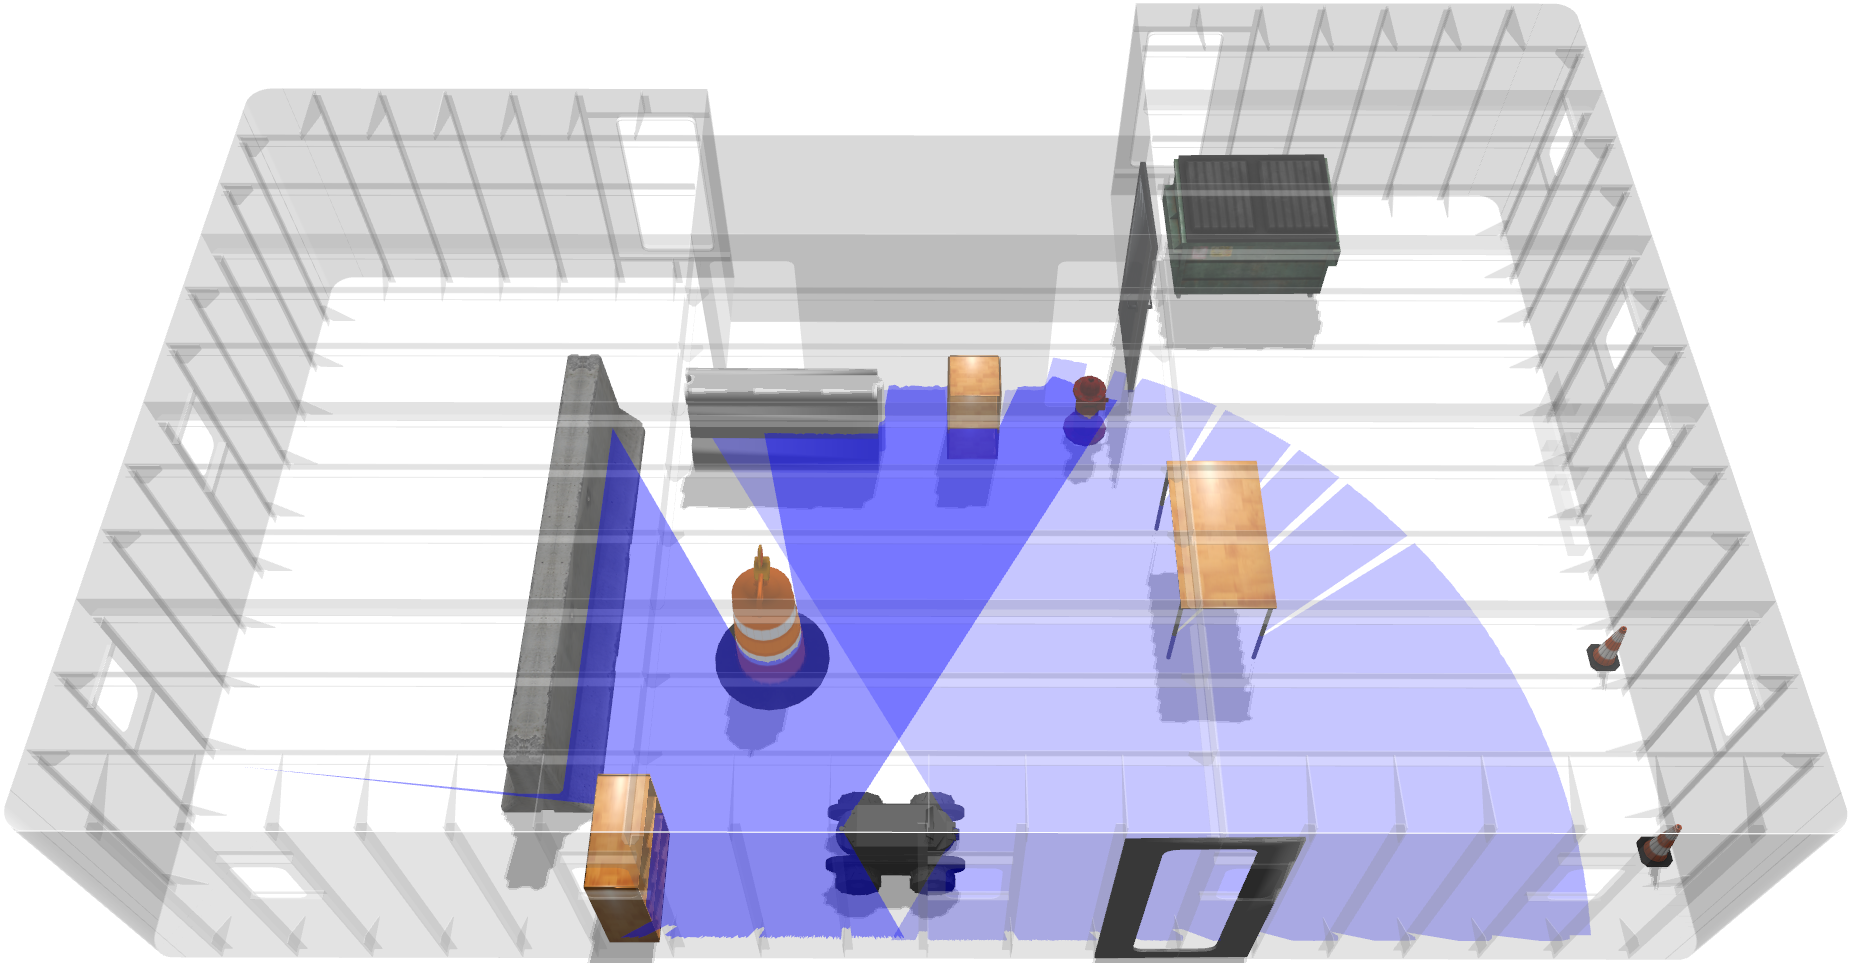
\includegraphics[width=\textwidth]{localization-system-evaluation/testing-environments/guardian-environment-cluttered}
	\end{subfigure}
	\begin{subfigure}[ht]{0.4\textwidth}
		\centering
		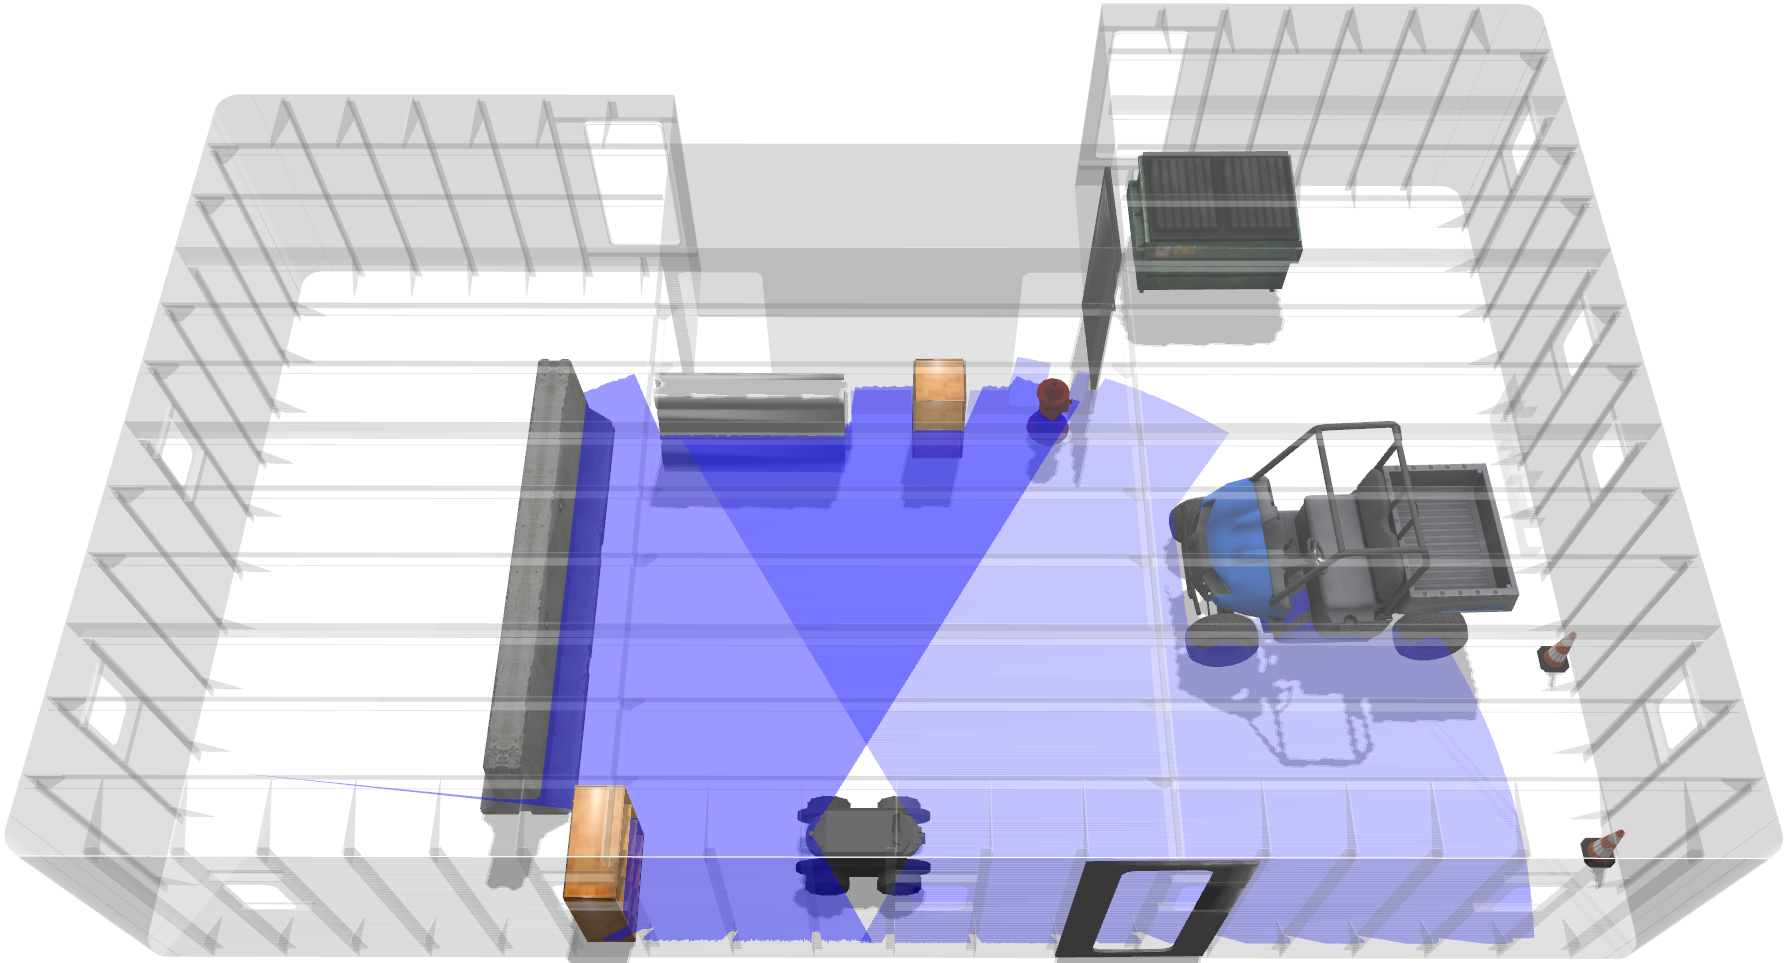
\includegraphics[width=\textwidth]{localization-system-evaluation/testing-environments/guardian-environment-cluttered-dynamic}
	\end{subfigure}
	\caption{Guardian cluttered (top) and dynamic (bottom) testing environments}
	\label{fig:localization-system-evaluation_guardian-tests-environment-cluttered}
\end{figure}



\subsubsection{Pioneer in industrial hall}

One of the datasets presented in \cite{Sturm2012} is a industrial hall consisting of a large room with several tables and objects spread around. Four tests were performed with a Pioneer 3-DX in this environment. The first was a 360º path with few camera supports in the middle of the room, while the remaining 3 were done with a lot of large objects, that significantly reduced the field of view of the robot laser (as can be seen in \Cref{fig:localization-system-evaluation_industrial-hall}).

\begin{figure}[ht]
	\centering
	\begin{subfigure}[ht]{0.37\textwidth}
		\centering
		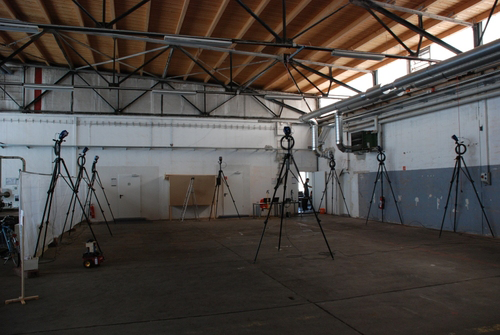
\includegraphics[width=0.95\textwidth]{localization-system-evaluation/testing-environments/industrial-hall-1}
	\end{subfigure}
	\begin{subfigure}[ht]{0.44\textwidth}
		\centering
		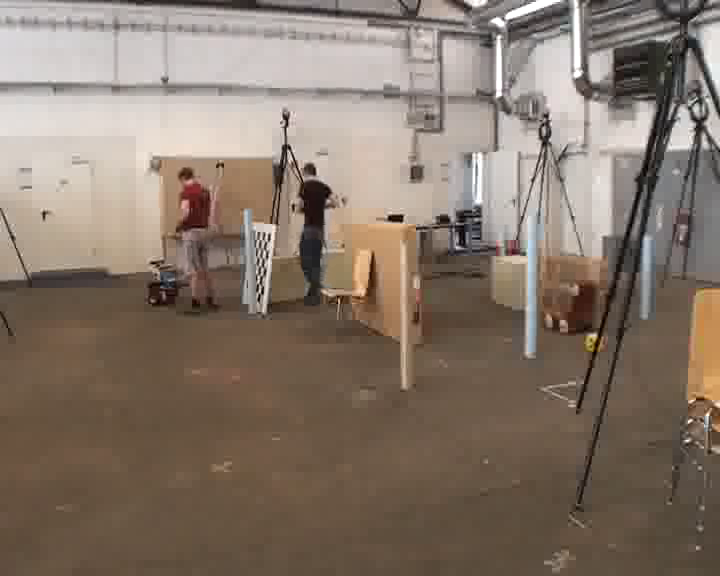
\includegraphics[width=0.8\textwidth]{localization-system-evaluation/testing-environments/industrial-hall-2}
	\end{subfigure}
	\caption{Industrial hall with (top) and without (bottom) objects in the center \cite{Sturm2012}}
	\label{fig:localization-system-evaluation_industrial-hall}
\end{figure}



\subsubsection{Kinect in flying arena}

The flying arena dataset introduced in \cite{Pomerleau2011} and shown in \Cref{fig:localization-system-evaluation_flying-arena} is a large room in which several objects were added to test 6 \gls{dof} pose tracking. In these tests the Kinect was moved by the operator in three different paths. The first was a smooth fly movement over the testing scene, while the other two aimed to test paths with mainly translations and rotations. This environment had a ground truth provided by Vicon cameras\footnote{\url{http://www.vicon.com/}} and according to the authors of the dataset \cite{Pomerleau2011} it had sub-centimeter accuracy.

\begin{figure}[H]
	\centering
	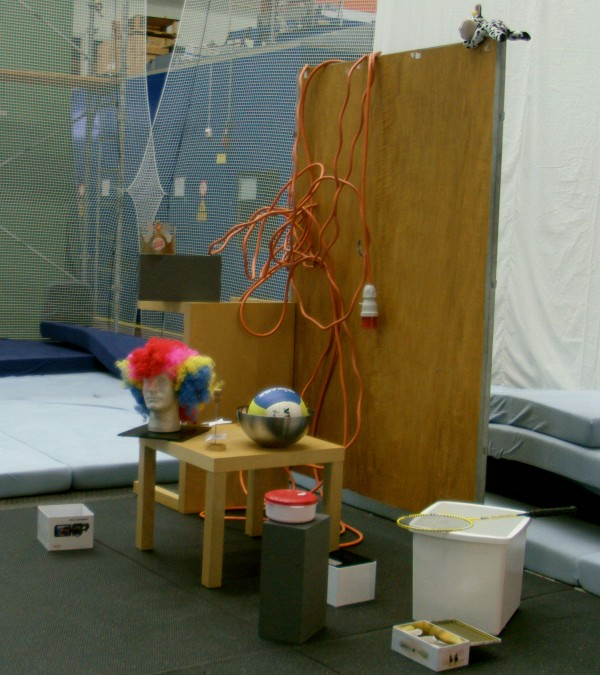
\includegraphics[width=0.35\textwidth]{localization-system-evaluation/testing-environments/kinect-flying-arena}
	\caption{Flying arena environment \cite{Pomerleau2011}}
	\label{fig:localization-system-evaluation_flying-arena}
\end{figure}

\section{3 \glsentrytext{dof} localization system tests}\label{sec:planar-localization-system-tests}


\subsection{Overview}

The main results of the 3 \gls{dof} tests performed with the \gls{drl} system (performing localization only with a given initial pose) are presented in \cref{tab:localization-system-evaluation_3-dof-results,tab:localization-system-evaluation_3-dof-results-odometry-amcl}. They summarize each test by fitting a normal distribution to each evaluation metric. They were retrieved with a known initial pose and used \gls{icp} point-to-point as tracking algorithm. The Jarvis and Pioneer tests had a map built using the localization system in mapping mode and were manually corrected to achieve a resolution of 10 and 25 mm respectively (shown in \Cref{fig:localization-system-evaluation_lab-10mm} and \Cref{fig:localization-system-evaluation_drl-corrected} respectively). The Guardian tests relied on a map built from the \gls{cad} model with resolution of 2 mm. Sensor data preprocessing relied on a voxel grid of 50 mm in order to reduce the impact of sensor measurement noise and also control the level of detail of the live point clouds. The initial pose estimation subsystem tests used \gls{sift} for keypoint selection, \gls{fpfh} for keypoint description and the feature matching algorithm described in \Cref{subsec:localization-system_feature-registration} to estimate the initial position and orientation of the robot (\Cref{fig:localization-system-evaluation_ship-interior-initial-pose-estimation-sift-fpfh-ransac-gicp-1} shows the accepted initial poses when the robot was in the lower right corner of the Guardian test environment and was given as the initial pose the large red arrow).

The next sections we will provide a brief analysis of the main 3 \gls{dof} results achieved with the \gls{drl} system. We will start by explaining how laser spherical interpolation can improve localization by mitigating point cloud deformation. Later on we will analyze the point cloud preprocessing stage and why it should be carefully tuned to the sensors and ambient geometry. Next we will present the mapping results and why it is necessary to have accurate environment representations in order to achieve precise localization. Finally it will be presented a global analysis of the tests results, in which the pose estimation accuracy achieved by the \gls{drl} system will be compared with the ground truth, odometry and \gls{amcl}.


\begin{sidewaystable*}
	\caption{3 \glsentrytext{dof} \glsentrytext{drl} localization test results}
	\tabulinesep = 0.8ex
	\setlength{\tabcolsep}{0.1em}
	\centering
	\scriptsize
	\begin{tabu} to \textwidth { X[m,c] X[m,c] X[m,c] X[1.7m,c] X[m,c] X[m,c] X[m,c] X[m,c] X[0.01m,c] X[m,c] X[m,c] X[0.01m,c] X[m,c] X[m,c] X[0.01m,c] X[m,c] X[m,c] X[0.01m,c] X[m,c] X[m,c] X[0.01m,c] X[m,c] }
		\hline
		\multicolumn{8}{c}{Test conditions} && \multicolumn{2}{c}{Translation error (mm)} && \multicolumn{2}{c}{Rotation error (degrees)} && \multicolumn{2}{c}{Outliers \% [0..100]} && \multicolumn{2}{c}{Processing time (ms)} && Cloud registrations \\
		\cline{1-8} \cline{10-11} \cline{13-14} \cline{16-17} \cline{19-20} \cline{22-22}
		Platform 																& Ambient 															& Path shape 											& Path velocities 		& kd-tree search radius (mm)  & Map cell resolution	& Spherical linear interpolation	& Nº scans / Nº lasers 	&& Mean    & Standard deviation && Mean  & Standard deviation 	&& Mean  & Standard deviation 	&& Mean   & Standard deviation 	&& Tracking recovery ratio \\ \hline
		\multirow{4}{0.05\textwidth}{\centering Jarvis robot} 					& \multirow{2}{0.05\textwidth}{\centering Cluttered} 				& \multirow{2}{0.05\textwidth}{\centering Rounded} 		& 5 cm/s 				& 0.2						  & 10 mm				&	Yes								& 1-4/1 				&& 4.281   & 2.264 				&& 0.441 & 0.070 				&& 24.35 & 5.17 				&& 11.776 & 12.265				&& 0/2154				   \\
																				&																	&														& 30 cm/s				& 0.2						  & 10 mm				&	Yes								& 1-4/1					&& 12.250  & 8.901				&& 0.535 & 0.414				&& 16.08 & 3.80					&& 21.295 &	8.352				&& 0/198				   \\ \tabucline[0.5pt on 3pt off 2pt]{2-3}
																				& \multirow{4}{0.05\textwidth}{\centering Cluttered dynamic}		& \multirow{4}{0.05\textwidth}{\centering Complex} 		& 5 cm/s 				& 0.2						  & 10 mm				&	Yes								& 1-4/1			 		&& 4.280   & 2.264 				&& 0.441 & 0.070 				&& 24.35 & 5.17 				&& 11.776 & 12.265				&& 0/3309				   \\
																				& 													 				& 														& 5 cm/s 				& 0.2						  & 10 mm				&	No								& 1-4/1 				&& 4.957   & 2.473 				&& 0.447 & 0.087 				&& 24.34 & 5.17 				&& 11.656 & 12.997				&& 0/3304				   \\
																				&																	&														& {50-30-50-10 cm/s}	& 0.2						  & 10 mm				&	Yes								& 1-4/1					&& 6.422   & 3.992				&& 0.397 & 0.099				&& 23.84 & 5.59					&& 13.376 &	13.316				&& 0/2371				   \\
																				&																	&														& {50-30-50-10 cm/s}	& 0.2						  & 10 mm				&	No								& 1-4/1					&& 8.884   & 8.740				&& 0.422 & 0.142				&& 24.14 & 6.18					&& 14.830 &	23.091				&& 34/2366				   \\ \tabucline[0.5pt on 3pt off 2pt]{1-3}
		\multirow{4}{0.05\textwidth}{\centering Pioneer robot}					& \multirow{4}{0.05\textwidth}{\centering Cluttered dynamic}		& 360º													& 23 cm/s				& 0.2						  & 25 mm				&	Yes								& 1/1					&& 20.105  & 10.814				&& 5.704 & 0.662				&& 11.71 & 3.37					&& 5.046  & 2.106				&& 0/671				   \\
																				&																	& SLAM 1												& 26 cm/s				& 0.2						  & 25 mm				&	Yes								& 1/1					&& 22.434  & 12.052				&& 5.429 & 0.676				&& 4.31  & 3.84					&& 4.569  & 2.530				&& 0/1441				   \\
																				&																	& SLAM 2												& 19 cm/s				& 0.2						  & 25 mm				&	Yes								& 1/1					&& 19.391  & 12.568				&& 5.518 & 0.818				&& 5.09  & 4.11					&& 4.650  & 2.180				&& 1/1065				   \\
																				&																	& SLAM 3												& 16 cm/s				& 0.2						  & 25 mm				&	Yes								& 1/1					&& 17.480  & 8.895				&& 5.455 & 0.732				&& 4.15  & 4.26					&& 4.388  & 2.526				&& 0/1044				   \\ \tabucline[0.5pt on 3pt off 2pt]{1-3}
		\multirow{10}{0.05\textwidth}{\centering Guardian simulator (Gazebo)} 	& \multirow{2}{0.05\textwidth}{\centering Static} 					& \multirow{10}{0.05\textwidth}{\centering Wall follower}& 5 cm/s 				& 0.05						  & 2 mm				&	Yes								& 2/2 					&& 2.642   & 0.463 				&& 0.016 & 0.023 				&& 0.0   & 0.0  				&& 5.723  & 1.868 				&& 0/2497				   \\
																				&  																	&														& 30 cm/s 				& 0.15						  & 2 mm				&	Yes								& 2-4/2					&& 4.654   & 3.893 				&& 0.044 & 0.070 				&& 0.0   & 0.0  				&& 7.784  & 3.178 				&& 0/429				   \\ \tabucline[0.5pt on 3pt off 2pt]{2-2}
																				& \multirow{2}{0.05\textwidth}{\centering Cluttered} 				&														& 5 cm/s 				& 0.02						  & 2 mm				&	Yes								& 2/2					&& 2.912   & 0.856 				&& 0.020 & 0.026 				&& 25.05 & 13.30 				&& 11.889 & 9.084 				&& 0/2500				   \\
																				&  																	&														& 30 cm/s 				& 0.2						  & 2 mm				&	Yes								& 2-4/2					&& 6.092   & 3.834 				&& 0.096 & 0.085 				&& 25.65 & 11.02 				&& 23.925 & 27.959 				&& 0/424				   \\ \tabucline[0.5pt on 3pt off 2pt]{2-2}
																				& \multirow{2}{0.05\textwidth}{\centering Cluttered dynamic}		&														& 5 cm/s 				& 0.05						  & 2 mm				&	Yes								& 2/2					&& 4.593   & 3.802 				&& 0.069 & 0.072 				&& 33.33 & 9.88  				&& 22.217 & 32.408 				&& 6/2428				   \\
																				&  																 	&														& 30 cm/s 				& 0.2						  & 2 mm				&	Yes								& 2-4/2					&& 5.897   & 4.452 				&& 0.095 & 0.104 				&& 27.28 & 13.04 				&& 24.409 & 33.459 				&& 0/416				   \\ \tabucline[0.5pt on 3pt off 2pt]{2-2}
																				& \multirow{4}{0.05\textwidth}{\centering Occluded wall}			&														& 5 cm/s 				& 0.15						  & 2 mm				&	Yes								& 2-4/2					&& 12.520  & 11.100 			&& 0.128 & 0.125 				&& 44.18 & 11.08  				&& 10.303 & 4.865 				&& 0/2376				   \\
																				&  																	&														& 5 cm/s 				& 0.50						  & 2 mm				&	Yes								& 2-4/2					&& 237.481 & 81.445 			&& 0.598 & 0.561 				&& 40.60 & 8.08 				&& 19.096 & 12.670 				&& 0/2376				   \\
																				& 																	&														& 30 cm/s 				& 0.15						  & 2 mm				&	Yes								& 2-4/2					&& 19.471  & 23.524				&& 0.144 & 0.132 				&& 46.94 & 10.36  				&& 12.240 & 6.045 				&& 0/435				   \\
																				&  																	&														& 30 cm/s 				& 0.50						  & 2 mm				&	Yes								& 2-4/2					&& 218.534 & 91.395 			&& 0.569 & 0.423 				&& 42.88 & 8.19 				&& 22.170 & 15.038 				&& 0/435				   \\
		\hline
	\end{tabu}
	\label{tab:localization-system-evaluation_3-dof-results}
	
	\bigskip
	
	\caption{3 \glsentrytext{dof} odometry and \glsentrytext{amcl} localization test results}
	\begin{tabu} to \textwidth { X[m,c] X[1.3m,c] X[m,c] X[1.7m,c] X[m,c] X[0.01m,c] X[m,c] X[m,c] X[0.01m,c] X[m,c] X[m,c] X[0.01m,c] X[m,c] X[m,c] X[0.01m,c] X[m,c] X[m,c] }
		\hline
		\multicolumn{5}{c}{Test conditions} && \multicolumn{2}{c}{Odometry translation error (mm)} && \multicolumn{2}{c}{Odometry rotation error (degrees)} && \multicolumn{2}{c}{\glsentrytext{amcl} translation error (mm)} && \multicolumn{2}{c}{\glsentrytext{amcl} rotation error (degrees)} \\
		\cline{1-5} \cline{7-8} \cline{10-11} \cline{13-14} \cline{16-17}
		Platform 																& Ambient 															& Path shape 											& Path velocities 		& Map cell resolution 	&& Mean   	& Standard deviation 	&& Mean  	& Standard deviation 	&& Mean  	& Standard deviation 	&& Mean   & Standard deviation \\ \hline
		\multirow{4}{0.05\textwidth}{\centering Jarvis robot} 					& \multirow{2}{0.05\textwidth}{\centering Cluttered} 				& \multirow{2}{0.05\textwidth}{\centering Rounded} 		& 5 cm/s 				& 10 mm					&& 25.353 	& 10.075 				&& 0.352 	& 0.206 				&& 51.417	& 20.829 				&& 0.442  & 0.174	\\
																				&																	&														& 30 cm/s				& 10 mm					&& 103.676	& 50.992				&& 2.173 	& 1.916					&& 81.368	& 36.548				&& 1.388  &	1.085	\\ \tabucline[0.5pt on 3pt off 2pt]{2-3}
																				& \multirow{2}{0.05\textwidth}{\centering Cluttered dynamic}		& \multirow{2}{0.05\textwidth}{\centering Complex} 		& 5 cm/s 				& 10 mm					&& 21.506 	& 11.937 				&& 0.535 	& 0.360 				&& 64.300	& 13.750 				&& 0.316  & 0.214	\\
																				&																	&														& 50-30-50-10 cm/s		& 10 mm					&& 124.269	& 79.775				&& 2.723 	& 1.496					&& 84.230	& 29.134				&& 0.595  &	0.581	\\ \tabucline[0.5pt on 3pt off 2pt]{1-3}
		\multirow{4}{0.05\textwidth}{\centering Pioneer robot}					& \multirow{4}{0.05\textwidth}{\centering Cluttered dynamic}		& 360º													& 23 cm/s				& 25 mm					&& 482.439	& 163.657				&& 12.810	& 4.468					&& 135.442	& 66.445				&& 6.462  & 1.290	\\
																				&																	& SLAM 1												& 26 cm/s				& 25 mm					&& 370.283 	& 163.734				&& 8.351 	& 2.825					&& 111.470 	& 46.783				&& 6.496  & 1.386	\\
																				&																	& SLAM 2												& 19 cm/s				& 25 mm					&& 686.983 	& 361.666				&& 11.333 	& 5.423					&& 95.537  	& 47.560				&& 6.957  & 2.294	\\
																				&																	& SLAM 3												& 16 cm/s				& 25 mm					&& 295.714 	& 151.793				&& 8.858 	& 3.331					&& 108.690 	& 52.341				&& 6.463  & 1.363	\\ \tabucline[0.5pt on 3pt off 2pt]{2-3}
		\multirow{2}{0.05\textwidth}{\centering Guardian simulator (Gazebo)}	& \multirow{2}{0.05\textwidth}{\centering Occluded wall}			& \multirow{2}{0.05\textwidth}{\centering Wall follower}& 5 cm/s				& 2 mm					&& 590.541	& 486.260				&& 2.610	& 2.779					&& 538.565	& 439.726				&& 0.779  & 1.097	\\
																				&																	& 														& 30 cm/s				& 2 mm					&& 529.209 	& 386.532				&& 1.056 	& 1.309					&& 464.510 	& 356.744				&& 0.215  & 0.167	\\
		\hline
	\end{tabu}
	\label{tab:localization-system-evaluation_3-dof-results-odometry-amcl}
\end{sidewaystable*}


\subsection{Laser assembly with spherical linear interpolation}

The localization system was designed to operate with any kind of point cloud sensors. For the particular case of data retrieved using \glspl{lidar}, there is a very significant problem of point cloud deformation when the robot is moving or rotating at high speeds. This is due to the fact that a typical \gls{lidar} outputs laser scans at a very low rate (8-10 Hz), and as such, assuming that the robot isn't moving when capturing an entire scan will result in deformed point clouds.

Given that \gls{ros} outputs laser scans (an entire slice of laser measurements from the start to the end of its field of view), and the localization system doesn't have access to individual measurements as they arrive, then one way to mitigate this scan deformation is by using odometry and / or \gls{imu} information to update the robot pose between the pose corrections performed by the localization system. This allows to use spherical linear interpolation when converting from the raw measurements in polar coordinates into the required Cartesian coordinates in the map frame.

The laser scan deformation is negligible when the robot is moving very slowly. However, when traveling at higher speeds, the point cloud deformation poses a serious issue for map matching algorithms, and the usage of spherical linear interpolation is very important to mitigate it.

\Cref{fig:localization-system-evaluation_laser-deformation-1,fig:localization-system-evaluation_laser-deformation-2} were retrieved using the Jarvis robot with velocities of 50-30-50-10 cm/s and without using the spherical linear interpolation module. \Cref{fig:localization-system-evaluation_laser-deformation-1-corrected,fig:localization-system-evaluation_laser-deformation-2} were taken from the same test but now using the spherical linear interpolation module. In \Cref{fig:localization-system-evaluation_laser-deformation-1} can be seen that the laser measurements in front of the robot were deformed outwards, causing the points to be projected outside both walls. \Cref{fig:localization-system-evaluation_laser-deformation-2} shows a similar effect, which is now very noticeable since the first laser measurement isn't close to the last one. These deformations were severely diminished when the laser spherical linear interpolation module was used (as can be seen in \cref{fig:localization-system-evaluation_laser-deformation-1-corrected,fig:localization-system-evaluation_laser-deformation-2-corrected} respectively.

Analyzing the tests in \cref{tab:localization-system-evaluation_3-dof-results} associated to the \crefrange{fig:localization-system-evaluation_laser-deformation-1}{fig:localization-system-evaluation_laser-deformation-2-corrected} it can be seen that using the spherical linear interpolation module allowed to reduce the mean (from 8.88 mm to 6.42 mm) and standard deviation (from 8.74 mm to 3.99 mm) of the translation error and also reduced the mean (from 0.42º to 0.39º) and standard deviation (from 0.14º to 0.10º) of the rotation error. Moreover, given that the correction of deformation gives a point cloud more similar to the map, the usage of the spherical linear interpolation module also allowed to reduced the global computation time (mean from 14.83 ms to 13.38 ms and standard deviation from 23.09 ms to 13.32 ms).

The laser assembly parameters present in \cref{tab:localization-system-evaluation_3-dof-results,tab:localization-system-evaluation_3-dof-results-odometry-amcl} as "Nº scans / Nº lasers" have the meaning of how many laser scans were being merged into each published \emph{sensor\_msgs::PointCloud2} and from how many sensors those lasers scans were being generated. As such, a configuration of "2-4/2" means that the laser assembler was merging between 2 (moving fast) and 4 (moving slow) lasers scans depending on the velocity of the robot, and these laser scans were being generated by two \glspl{lidar} sensors (one in the front and another in the back of the robot).


\begin{figure}[H]
	\centering
	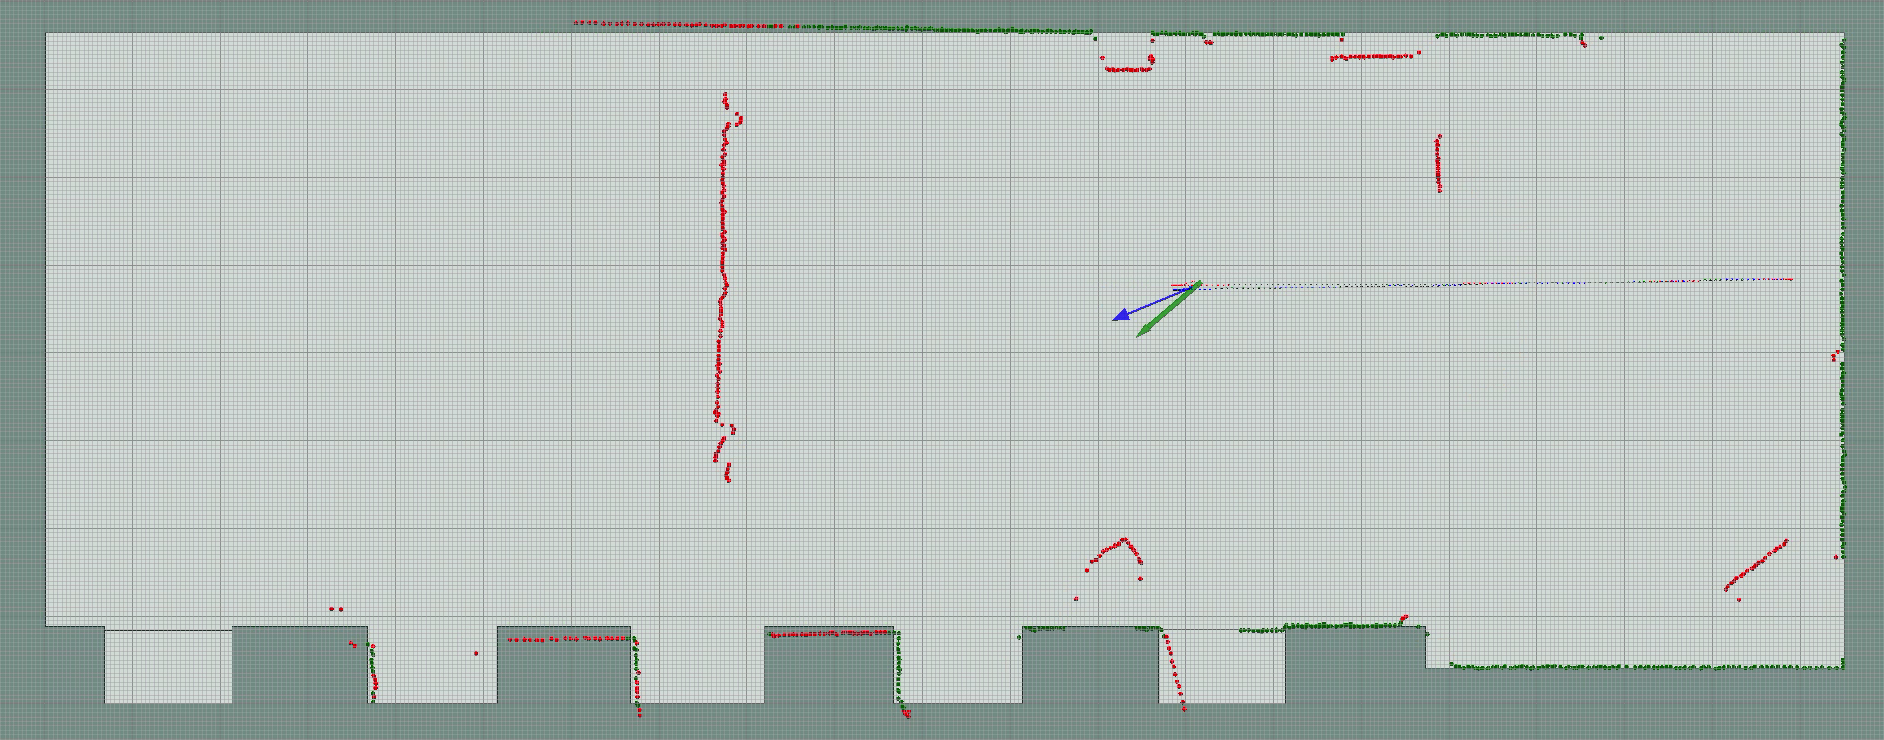
\includegraphics[width=0.49\textwidth]{localization-system-evaluation/tests-3dof/laser-spherical-interpolation/laser-deformation-1}
	\caption{Large laser deformation on opposite walls when the robot is rotating (grid with 1 m spacing)}
	\label{fig:localization-system-evaluation_laser-deformation-1}
\end{figure}

\begin{figure}[H]
	\centering
	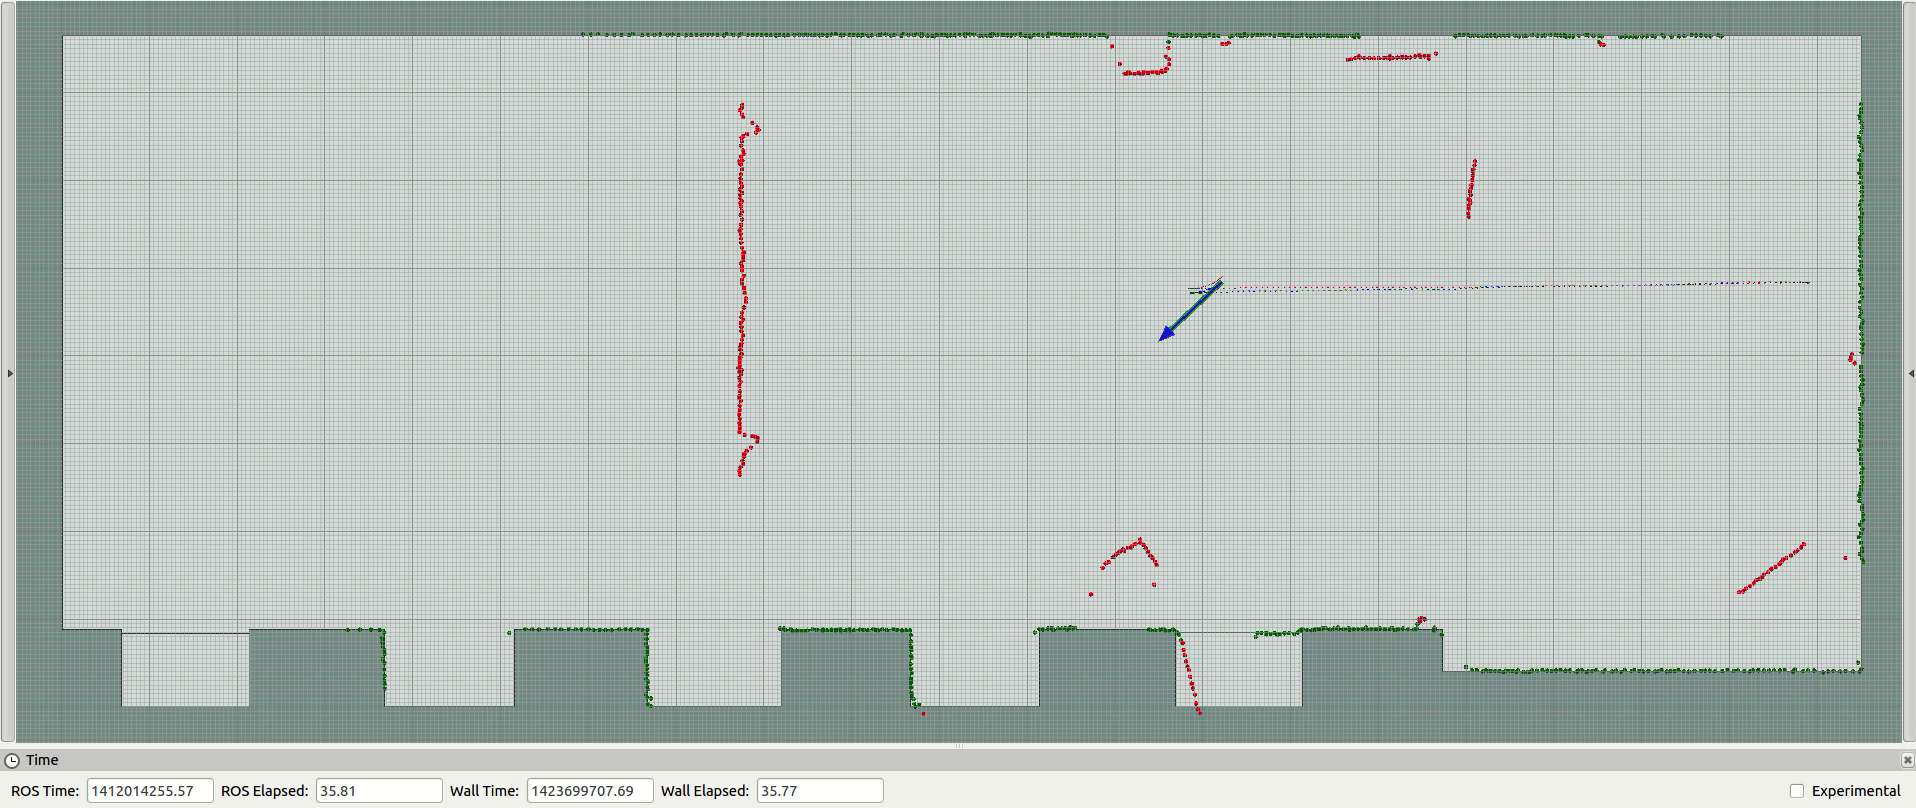
\includegraphics[width=0.49\textwidth]{localization-system-evaluation/tests-3dof/laser-spherical-interpolation/laser-deformation-1-corrected}
	\caption{Correction of the large laser deformation on opposite walls with spherical linear interpolation  (grid with 1 m spacing)}
	\label{fig:localization-system-evaluation_laser-deformation-1-corrected}
\end{figure}


\begin{figure}[H]
	\centering
	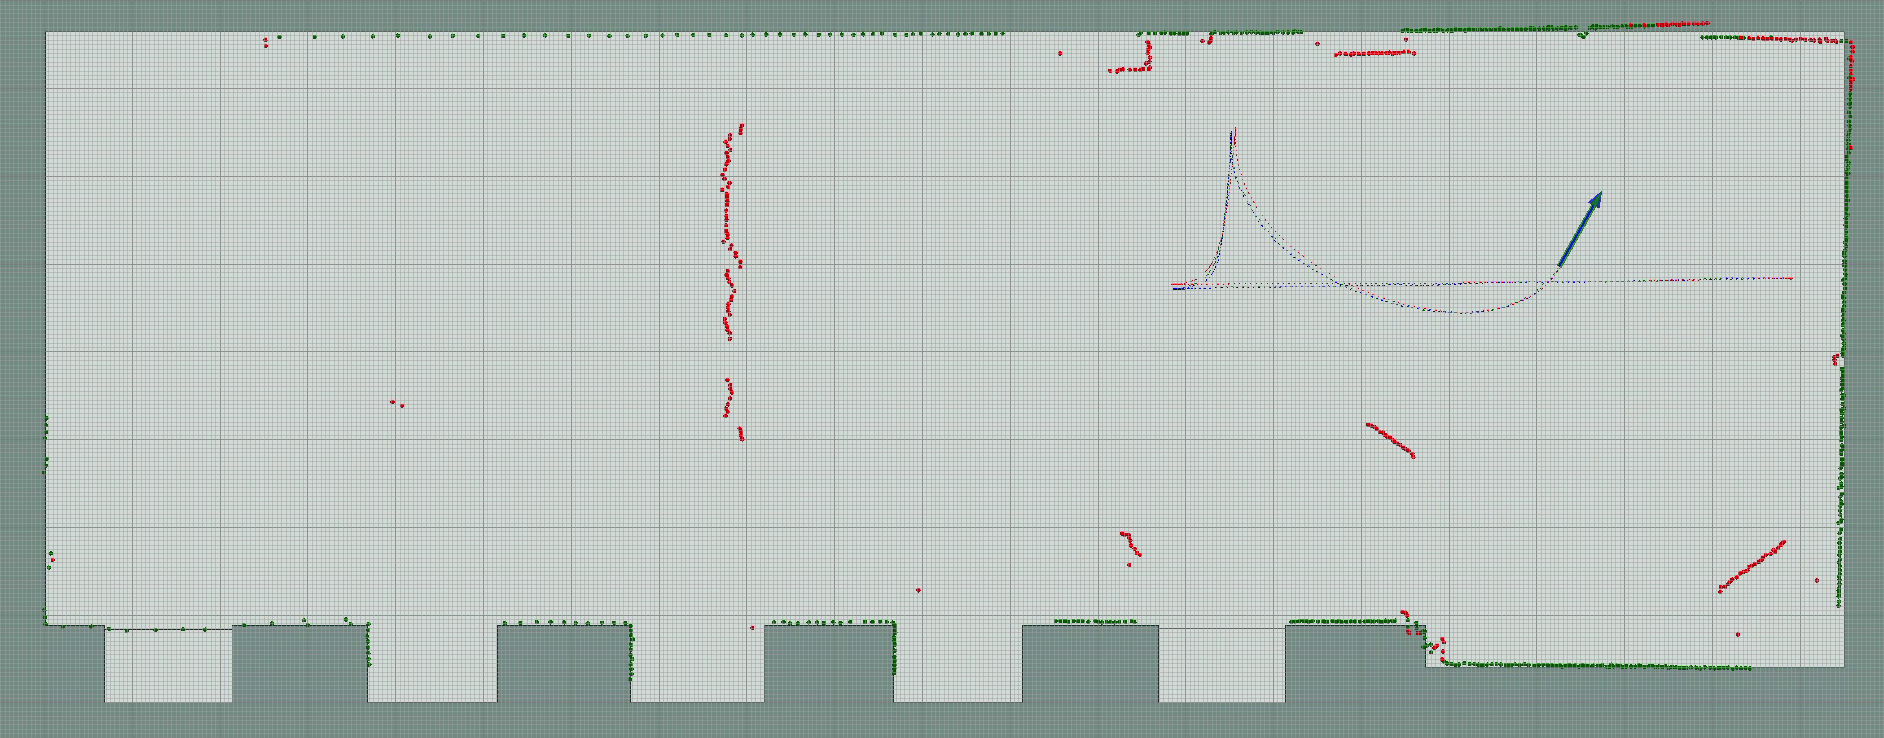
\includegraphics[width=0.49\textwidth]{localization-system-evaluation/tests-3dof/laser-spherical-interpolation/laser-deformation-2}
	\caption{Laser deformation when the robot is rotating  (grid with 1 m spacing)}
	\label{fig:localization-system-evaluation_laser-deformation-2}
\end{figure}

\begin{figure}[H]
	\centering
	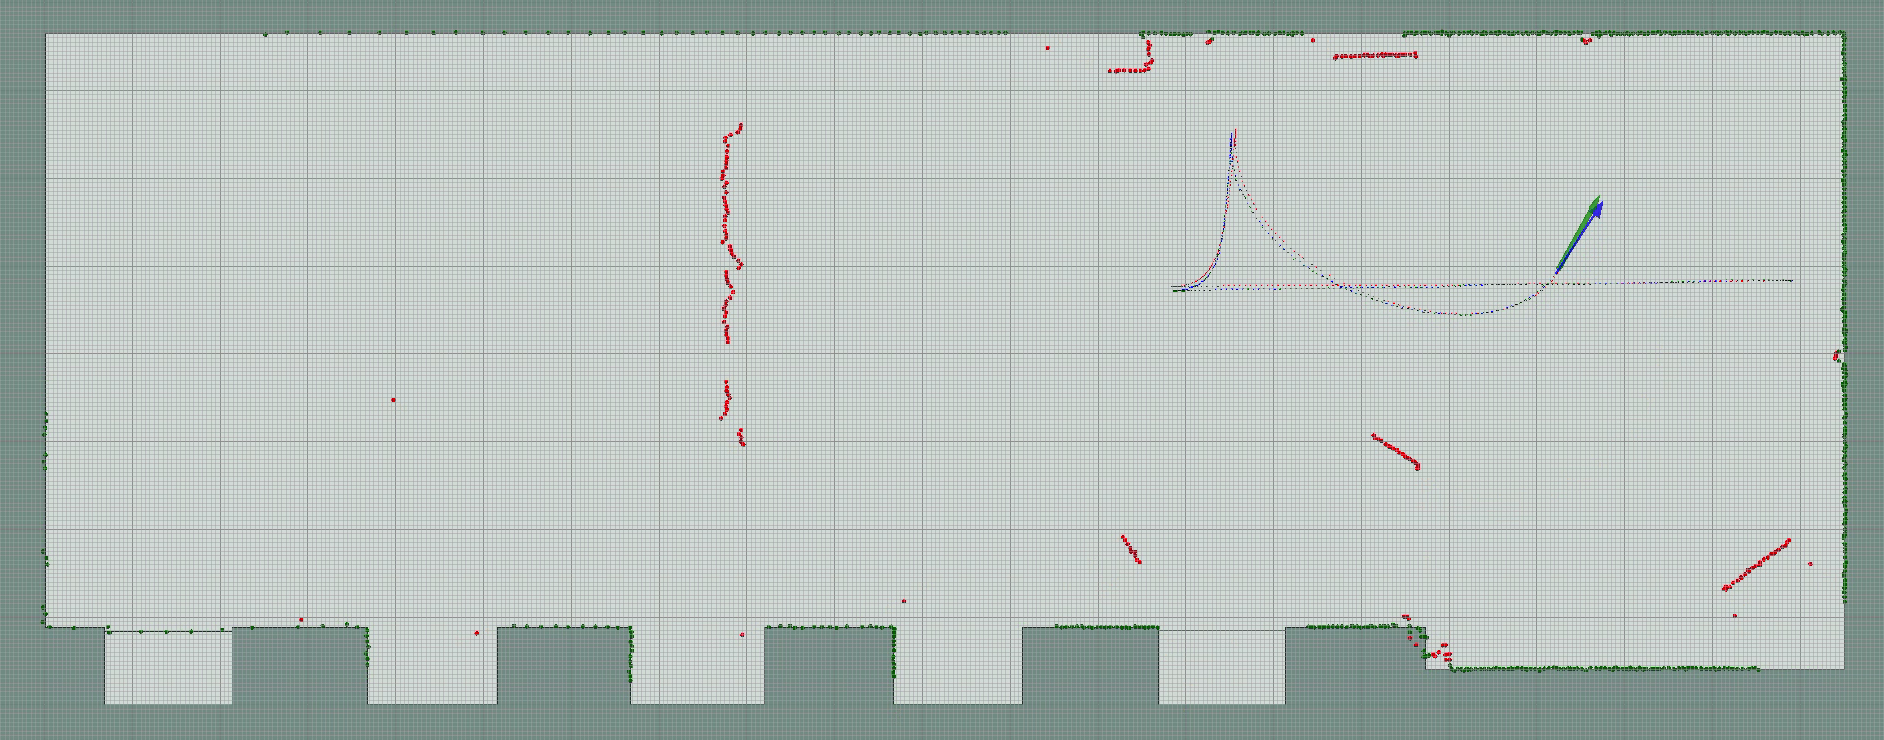
\includegraphics[width=0.49\textwidth]{localization-system-evaluation/tests-3dof/laser-spherical-interpolation/laser-deformation-2-corrected}
	\caption{Correction of the laser deformation with spherical linear interpolation  (grid with 1 m spacing)}
	\label{fig:localization-system-evaluation_laser-deformation-2-corrected}
\end{figure}



\subsection{Point cloud preprocessing}

The statistical error of the lasers can be mitigated by merging several laser scans before performing a point cloud registration. This is based on the fact that a considerable amount of laser noise results in measurements oscillating around the true distance to the obstacles, and as such, the effective measurement error can be significantly reduced by retrieving the centroids of a voxel grid applied over the laser data. However, assembling too much laser scans can lead to worse pose tracking if the robot is moving at high speeds, because the lasers would be projected into the map frame with a high position error (because odometry accuracy decreases when the robot speed increases and the localization system will not correct it). As such, the implemented laser assembler supports dynamic reconfiguration of the number of laser scans to assemble (or the period of assembly time) based on the robot estimated velocity. This feature besides improving the pose tracking, it also allows a navigation supervisor to regulate the rate at which the localization system operates. This can be very useful for mobile robot manipulators because the localization system can have a high update rate when the robot is moving fast and a low update rate when it is moving slower or when it is stopped. This allows a more efficient usage of the platform hardware resources while also improving the localization system accuracy.

Besides reducing the sensor measurement errors, this processing stage also allows the removal of laser shadow points caused by veiling, or small cluster of points that may be associated with temporary objects / people. However these filters can take some time to compute given the intensive usage of point neighbors searches. For typical usage scenarios of a mobile robot manipulator, the voxel grid and random sampling filters are usually enough to control the computational resources that will be required by the registration algorithms while also improving robustness against sensor noise.



\subsection{Point cloud registration}

Looking at the results from \cref{tab:localization-system-evaluation_3-dof-results,tab:localization-system-evaluation_3-dof-results-odometry-amcl}, the poses from \Cref{fig:localization-system-evaluation_complex-path-with-outliers-50-30-50-10cm-per-sec-velocity-1-4-scans-paths}, the laser assembly figures shown in \cref{fig:localization-system-evaluation_complex-path-with-outliers-50-30-50-10cm-per-sec-velocity-1-4-scans-drl-cumulative,fig:localization-system-evaluation_complex-path-with-outliers-50-30-50-10cm-per-sec-velocity-1-4-scans-amcl-cumulative} and the translation / rotation error graphs presented from \crefrange{fig:localization-system-evaluation_complex-path-with-outliers-50-30-50-10cm-per-sec-velocity-1-4-translation-error-amcl}{fig:localization-system-evaluation_complex-path-with-outliers-50-30-50-10cm-per-sec-velocity-1-4-rotation-error} (from the Jarvis test in the complex path at high velocities), it can be seen that the localization system can register point clouds with much more accuracy than the \gls{amcl} \gls{ros} package (\gls{amcl} was using at most 5000 particles). For the test shown in \cref{fig:localization-system-evaluation_complex-path-with-outliers-50-30-50-10cm-per-sec-velocity-1-4-scans-paths}, the \gls{drl} system was 13.12 times more accurate than the \gls{amcl} package in computing the robot position (achieved 6.422 mm of mean translation error while \gls{amcl} had 84.23 mm) and was also 1.5 times more accurate than the \gls{amcl} package in computing the robot orientation (achieved 0.397º of mean rotation error while \gls{amcl} had 0.595º).

The most common problems that seemed to affect the registration algorithms of the \gls{drl} system were the point cloud deformation (usually when there is unreliable odometry information, which typically occurs when the robot is moving with high velocities / accelerations), laser measurements errors, unknown objects close to the known reference point cloud and also low resolution maps. The localization system can tolerate these problems by having a default pipeline configuration for the normal operation of the robot, another for temporary tracking recovery and yet another for initial pose estimation.

The switch between the localization system operation modes using the point cloud registration analysis proved to be a very intuitive and fast process to setup and the overall system configurations seemed to be generic enough to be reused in several types of environments, with different robots equipped with varying types of sensors. Such ease of configuration allows the fast deployment of robots and gives a high confidence that the localization system will remain accurate even in challenging environments. This is not the case with systems such as \gls{amcl}, given that they are very dependent on the odometry and laser models, and as such, require constant retuning when one of these models change.

The ability to switch registration algorithms at runtime based on the quality of the estimated pose proved to be an efficient and flexible architecture choice, since it allowed high precision pose tracking with fast registration algorithms and occasional pose tracking recovery with more robust methods / configurations (which happened more often in the tests at higher velocities, in which the odometry was significantly worse).

The initial pose estimation using feature matching was very reliable and successfully found the robot location even in low feature surroundings (as can be seen in \cref{fig:localization-system-evaluation_jarvis-initial-pose-estimation-sift-fpfh-ransac-gicp-1,fig:localization-system-evaluation_ship-interior-initial-pose-estimation-sift-fpfh-ransac-gicp-1}). Moreover, the output of the accepted initial pose estimations allows the detection of similar map locations by a navigation supervisor, which can then plot a path to disambiguate the initial pose guess and avoid dangerous operations at a wrong position.

\Crefrange{fig:localization-system-evaluation_jarvis-initial-pose-estimation-sift-fpfh-ransac-gicp-1}{fig:localization-system-evaluation_ship-interior-initial-pose-estimation-sift-fpfh-ransac-gicp-2} show the accepted initial pose estimations using the global localization subsystem presented in \cref{subsec:localization-system_feature-registration}.

The blue circles presented in \Cref{fig:localization-system-evaluation_jarvis-initial-pose-estimation-sift-fpfh-ransac-gicp-1} represent the keypoints of the live point cloud in the robot start up position, while the violet circles are the reference point cloud keypoints. The green circles are the live point cloud laser measurements after performing the initial pose estimation and registration refinement.


\begin{figure}[H]
	\centering
	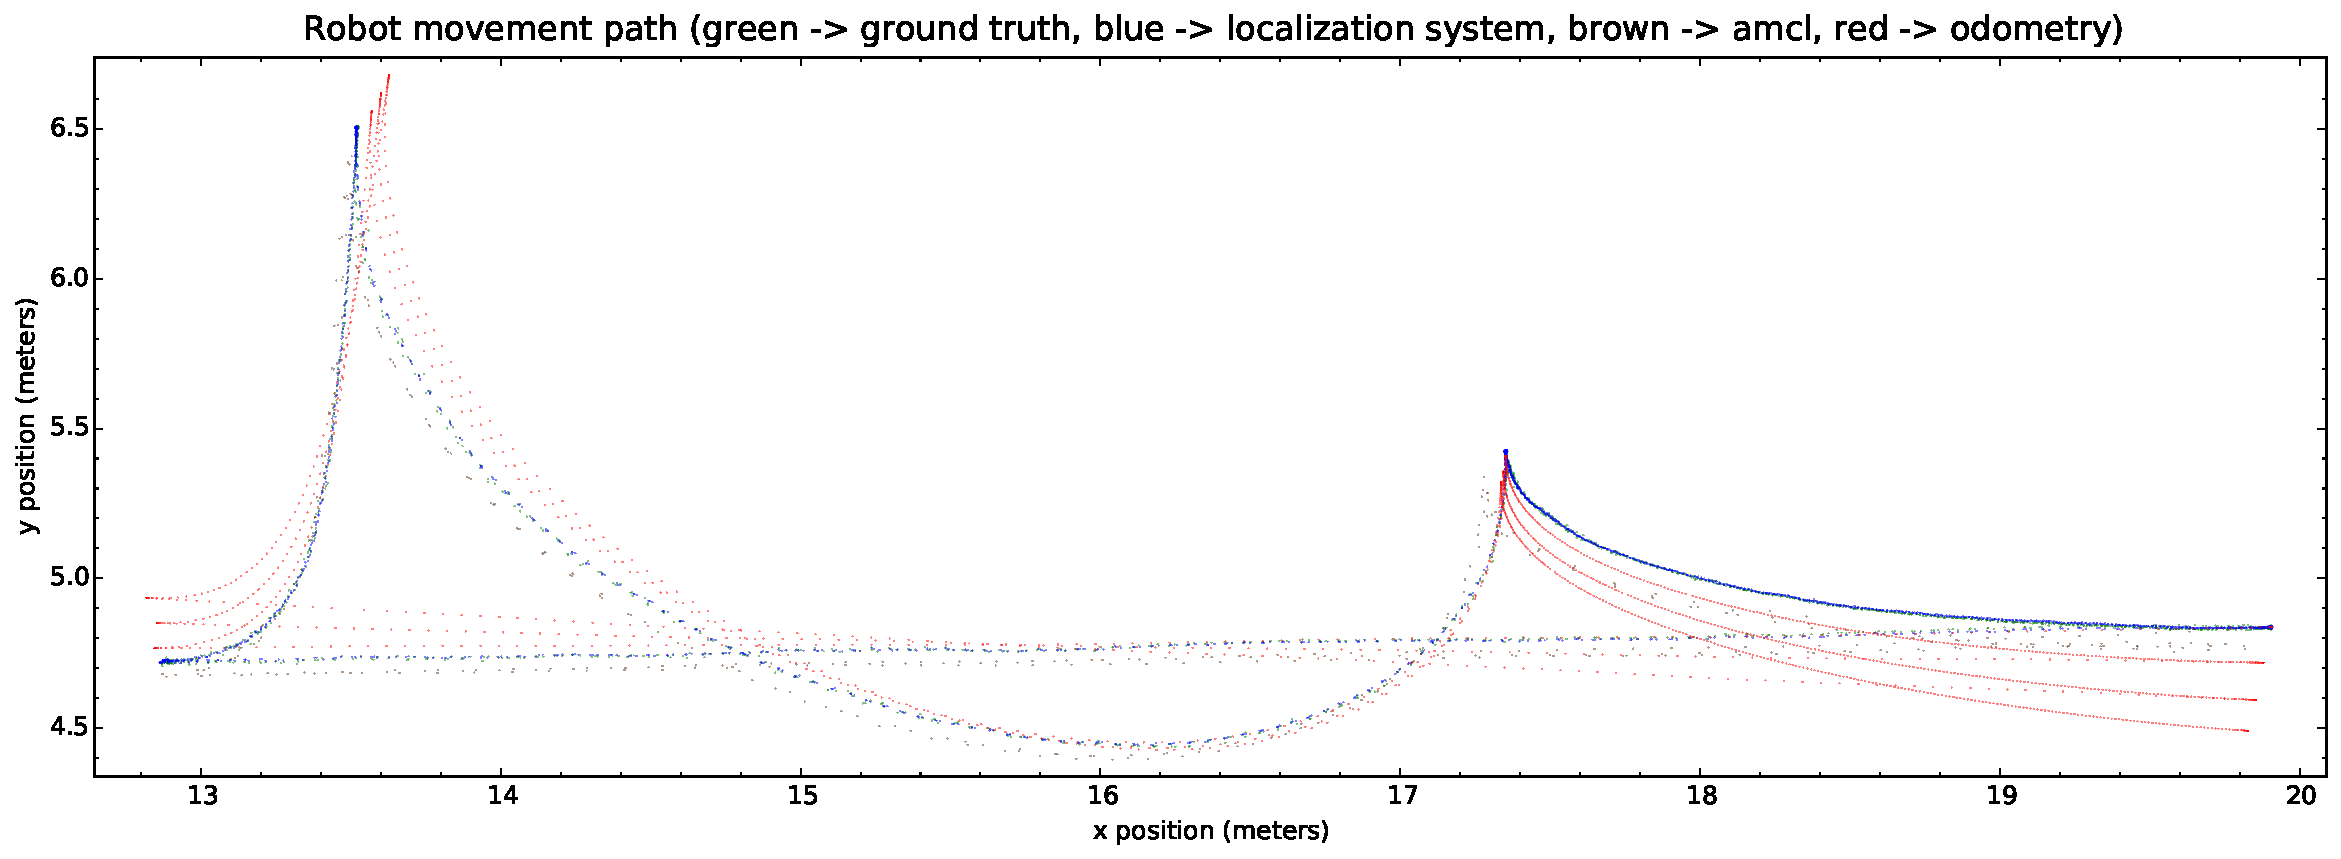
\includegraphics[trim={0 0 0 1cm}, clip, width=0.45\textwidth]{localization-system-evaluation/tests-3dof/jarvis-robot/complex-outliers-50-30-50-10-1-4-scans/graphs/robot-movement-path-with-odometry-and-amcl}
	\caption{Poses estimated by the ground truth, localization system, \glsentrytext{amcl} and odometry}
	\label{fig:localization-system-evaluation_complex-path-with-outliers-50-30-50-10cm-per-sec-velocity-1-4-scans-paths}
\end{figure}

\begin{figure}[H]
	\centering
	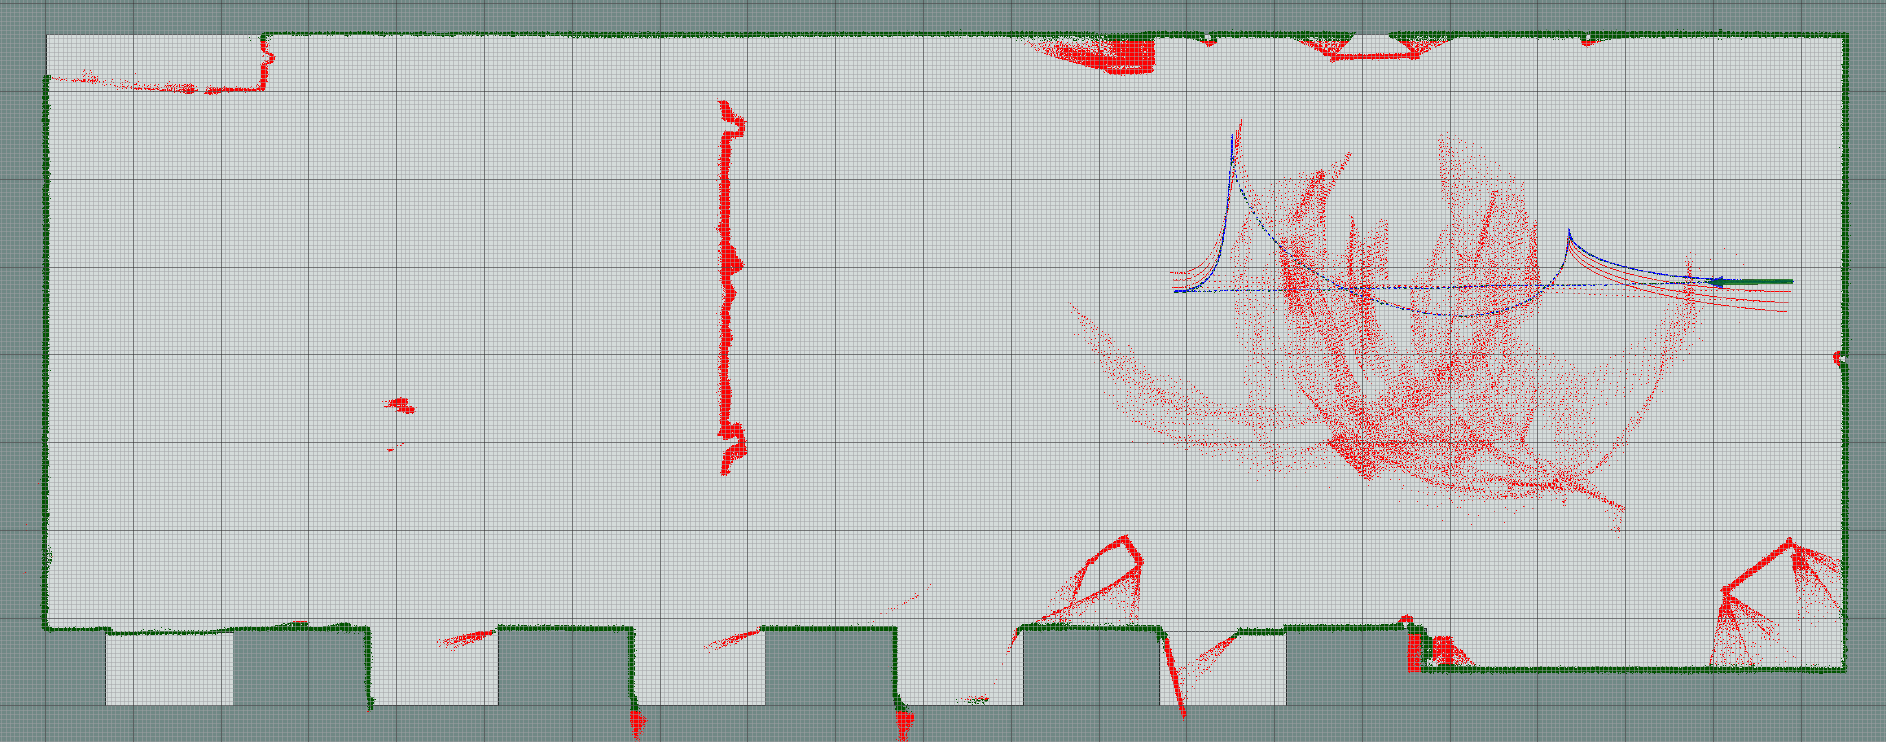
\includegraphics[width=0.45\textwidth]{localization-system-evaluation/tests-3dof/jarvis-robot/complex-outliers-50-30-50-10-1-4-scans/drl-cumulative}
	\caption{Laser scans assembled on top of the map using the localization system poses (grid with 1 m spacing)}
	\label{fig:localization-system-evaluation_complex-path-with-outliers-50-30-50-10cm-per-sec-velocity-1-4-scans-drl-cumulative}
\end{figure}

\begin{figure}[H]
	\centering
	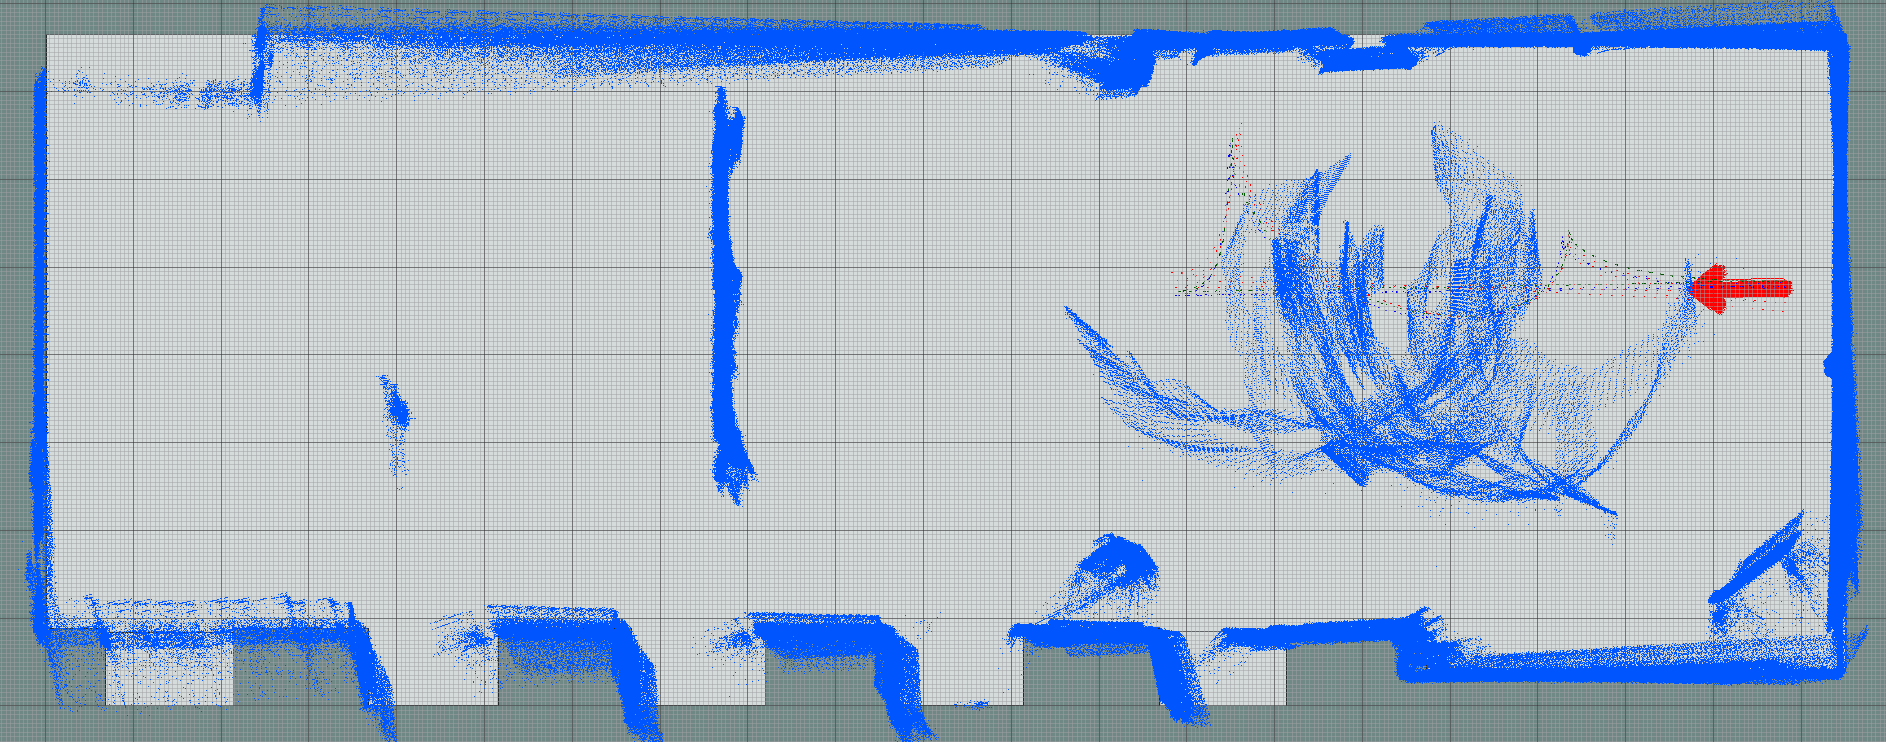
\includegraphics[width=0.45\textwidth]{localization-system-evaluation/tests-3dof/jarvis-robot/complex-outliers-50-30-50-10-1-4-scans/amcl-cumulative}
	\caption{Laser scans assembled on top of the map using the \glsentrytext{amcl} poses (grid with 1 m spacing)}
	\label{fig:localization-system-evaluation_complex-path-with-outliers-50-30-50-10cm-per-sec-velocity-1-4-scans-amcl-cumulative}
\end{figure}


\begin{figure}[H]
	\centering
	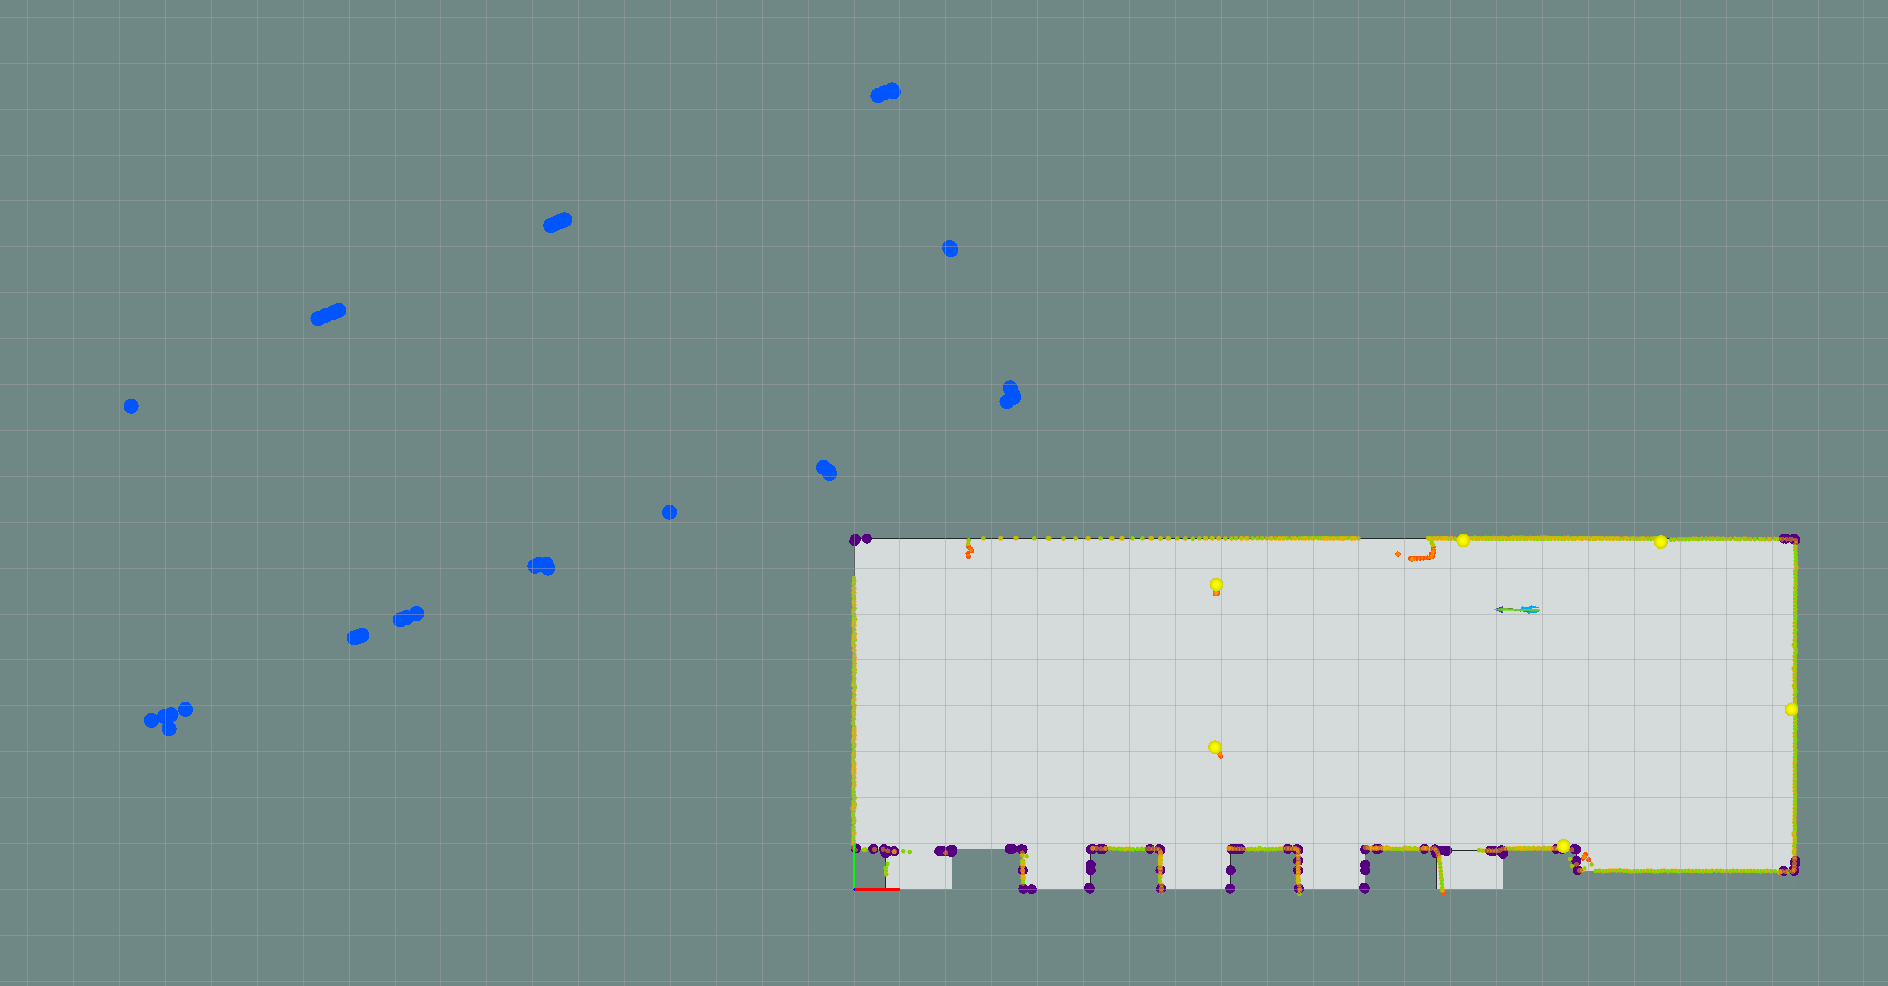
\includegraphics[width=0.45\textwidth]{localization-system-evaluation/tests-3dof/initial_pose_estimation/jarvis-initial-pose-estimation-sift-fpfh-ransac-gicp-1}
	\caption{Overview of initial pose estimation using feature matching in Jarvis environment (grid with 1 m spacing)}
	\label{fig:localization-system-evaluation_jarvis-initial-pose-estimation-sift-fpfh-ransac-gicp-1}
\end{figure}

%\begin{figure}[H]
%	\centering
%	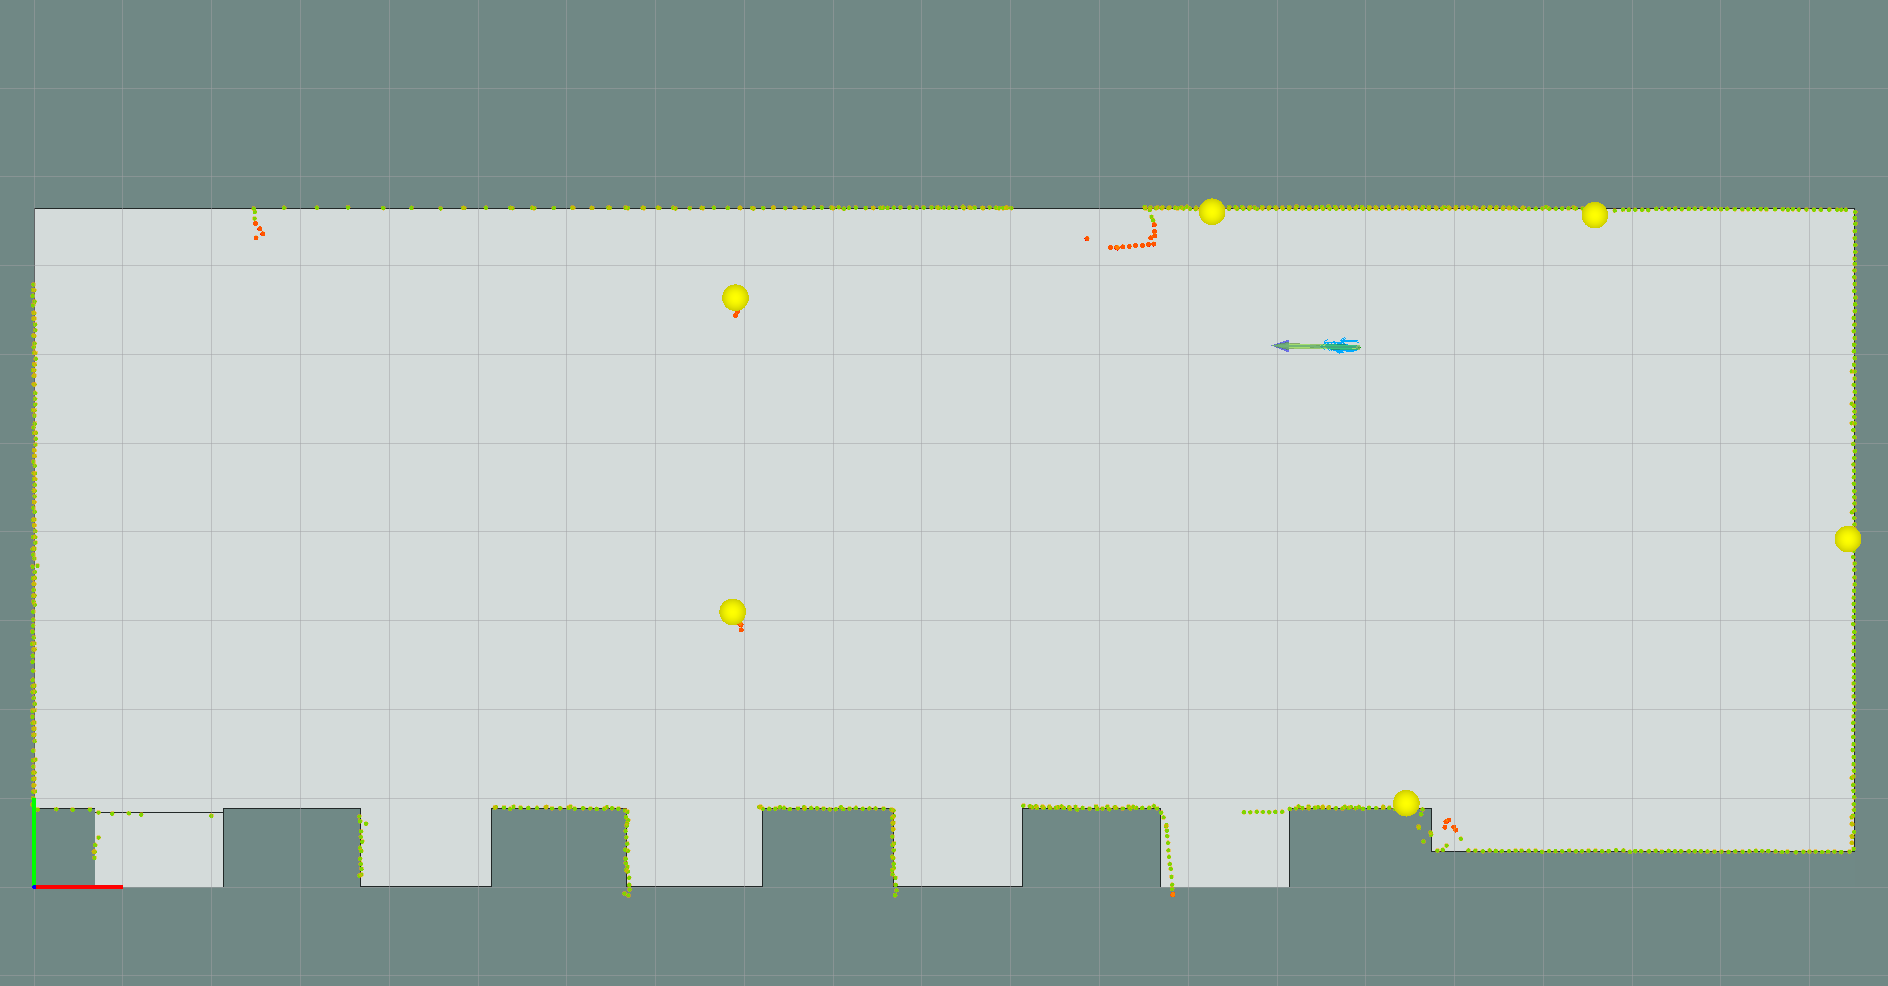
\includegraphics[width=0.45\textwidth]{localization-system-evaluation/tests-3dof/initial_pose_estimation/jarvis-initial-pose-estimation-sift-fpfh-ransac-gicp-3}
%	\caption{Initial pose estimation using feature matching in Guardian static environment (grid with 1 m spacing)}
%	\label{fig:localization-system-evaluation_jarvis-initial-pose-estimation-sift-fpfh-ransac-gicp-2}
%\end{figure}

\begin{figure}[H]
	\centering
	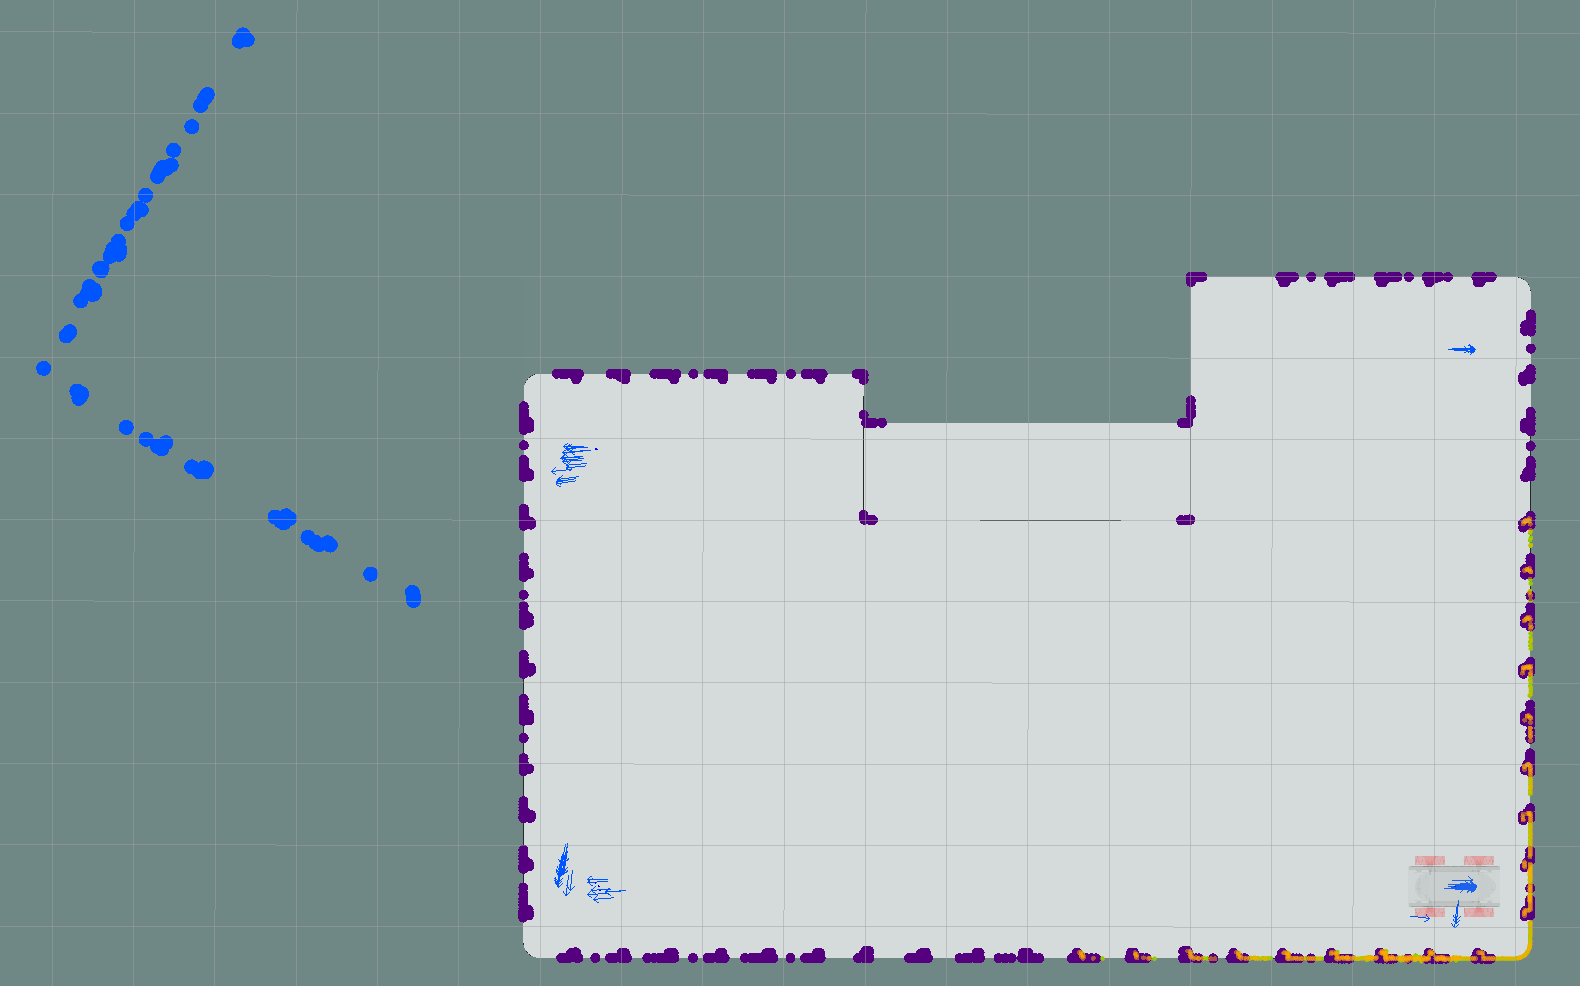
\includegraphics[width=0.45\textwidth]{localization-system-evaluation/tests-3dof/initial_pose_estimation/guardian-initial-pose-estimation-sift-fpfh-ransac-gicp-1}
	\caption{Overview of initial pose estimation using feature matching in Guardian static environment (grid with 1 m spacing)}
	\label{fig:localization-system-evaluation_ship-interior-initial-pose-estimation-sift-fpfh-ransac-gicp-1}
\end{figure}

%\begin{figure}[H]
%	\centering
%	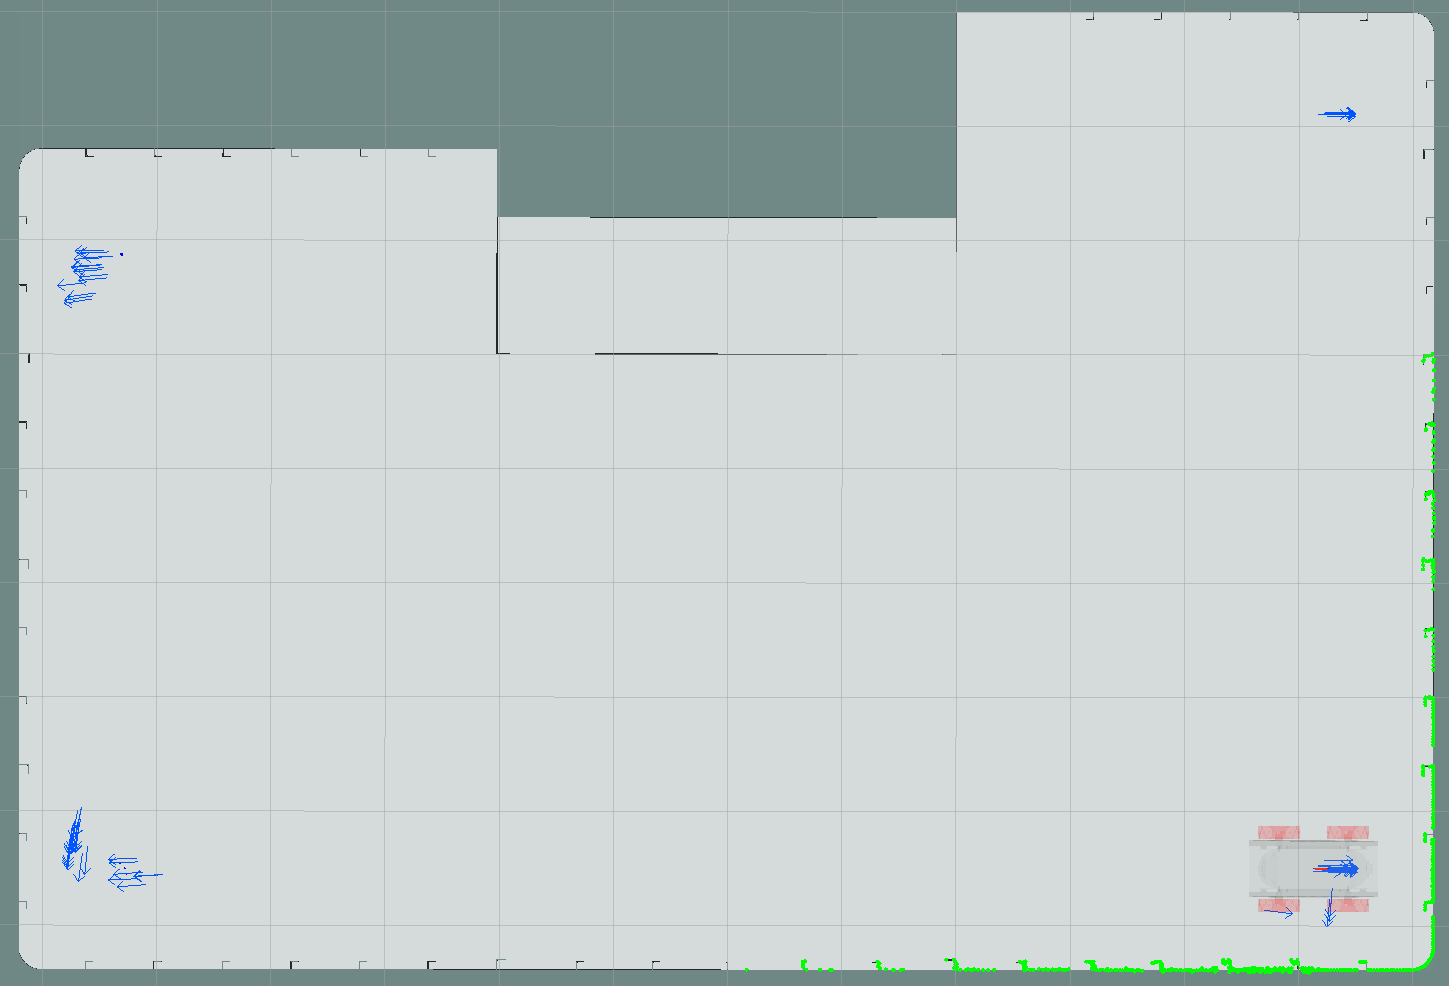
\includegraphics[width=0.45\textwidth]{localization-system-evaluation/tests-3dof/initial_pose_estimation/guardian-initial-pose-estimation-sift-fpfh-ransac-gicp-2}
%	\caption{Initial pose estimation using feature matching in Guardian static environment (grid with 1 m spacing)}
%	\label{fig:localization-system-evaluation_ship-interior-initial-pose-estimation-sift-fpfh-ransac-gicp-2}
%\end{figure}




\subsection{Translation and rotation errors}

By analyzing \cref{tab:localization-system-evaluation_3-dof-results,tab:localization-system-evaluation_3-dof-results-odometry-amcl} it can be seen that the proposed 3 \gls{dof} localization system can achieve pose tracking with less than 1 cm in translation error and less than 1 degree in rotation error when using a detailed map (10 mm cell resolution) and a sensor with good field of view (360º) and low sensor noise (15 mm). When using a sensor with low field of view (180º) and high sensor noise (35 mm), the \gls{drl} system still managed to achieve localization accuracy bellow the map resolution (translation error less than 2 cm and rotation error close to 5 degrees).

As expected, the tests at lower velocities had less mean error than the ones at higher speeds while requiring slightly less computation time. Also, the simulator tests had less mean error than the ones performed on the physical platforms. This is due to laser scan deformation that couldn't be simulated and also because the Gazebo simulator was only able to add Gaussian noise to the laser measurements. To compensate these limitations, the error in odometry and laser measurements in simulation was deliberately higher than the expected values for the physical platforms. This explains why the localization system needed more time to perform the pose estimations in the simulator tests. It can also be seen that adding unknown objects increased the mean error and required computation time while adding dynamic objects increased these values even further (given that a moving object appears in a laser scan as a deformed version of its static shape).

Comparing the results of the tests performed with Jarvis robot  with the tests of the Pioneer robot, it can be seen that even when severely reducing the laser range (from 80 to 6 meters), moving the robot in dynamic environments with large occluding objects and even when using a low resolution map (25 mm in the Pioneer tests vs 10 mm in the Jarvis tests), the localization system still managed to track the robot pose with mean translation error (17 mm) below the map resolution (25 mm).

These results show that the localization system can reliably achieve high accuracy pose tracking even in dynamic and challenging environments.

\begin{figure}[H]
	\centering
	\begin{minipage}[H]{0.49\textwidth}
		\centering
		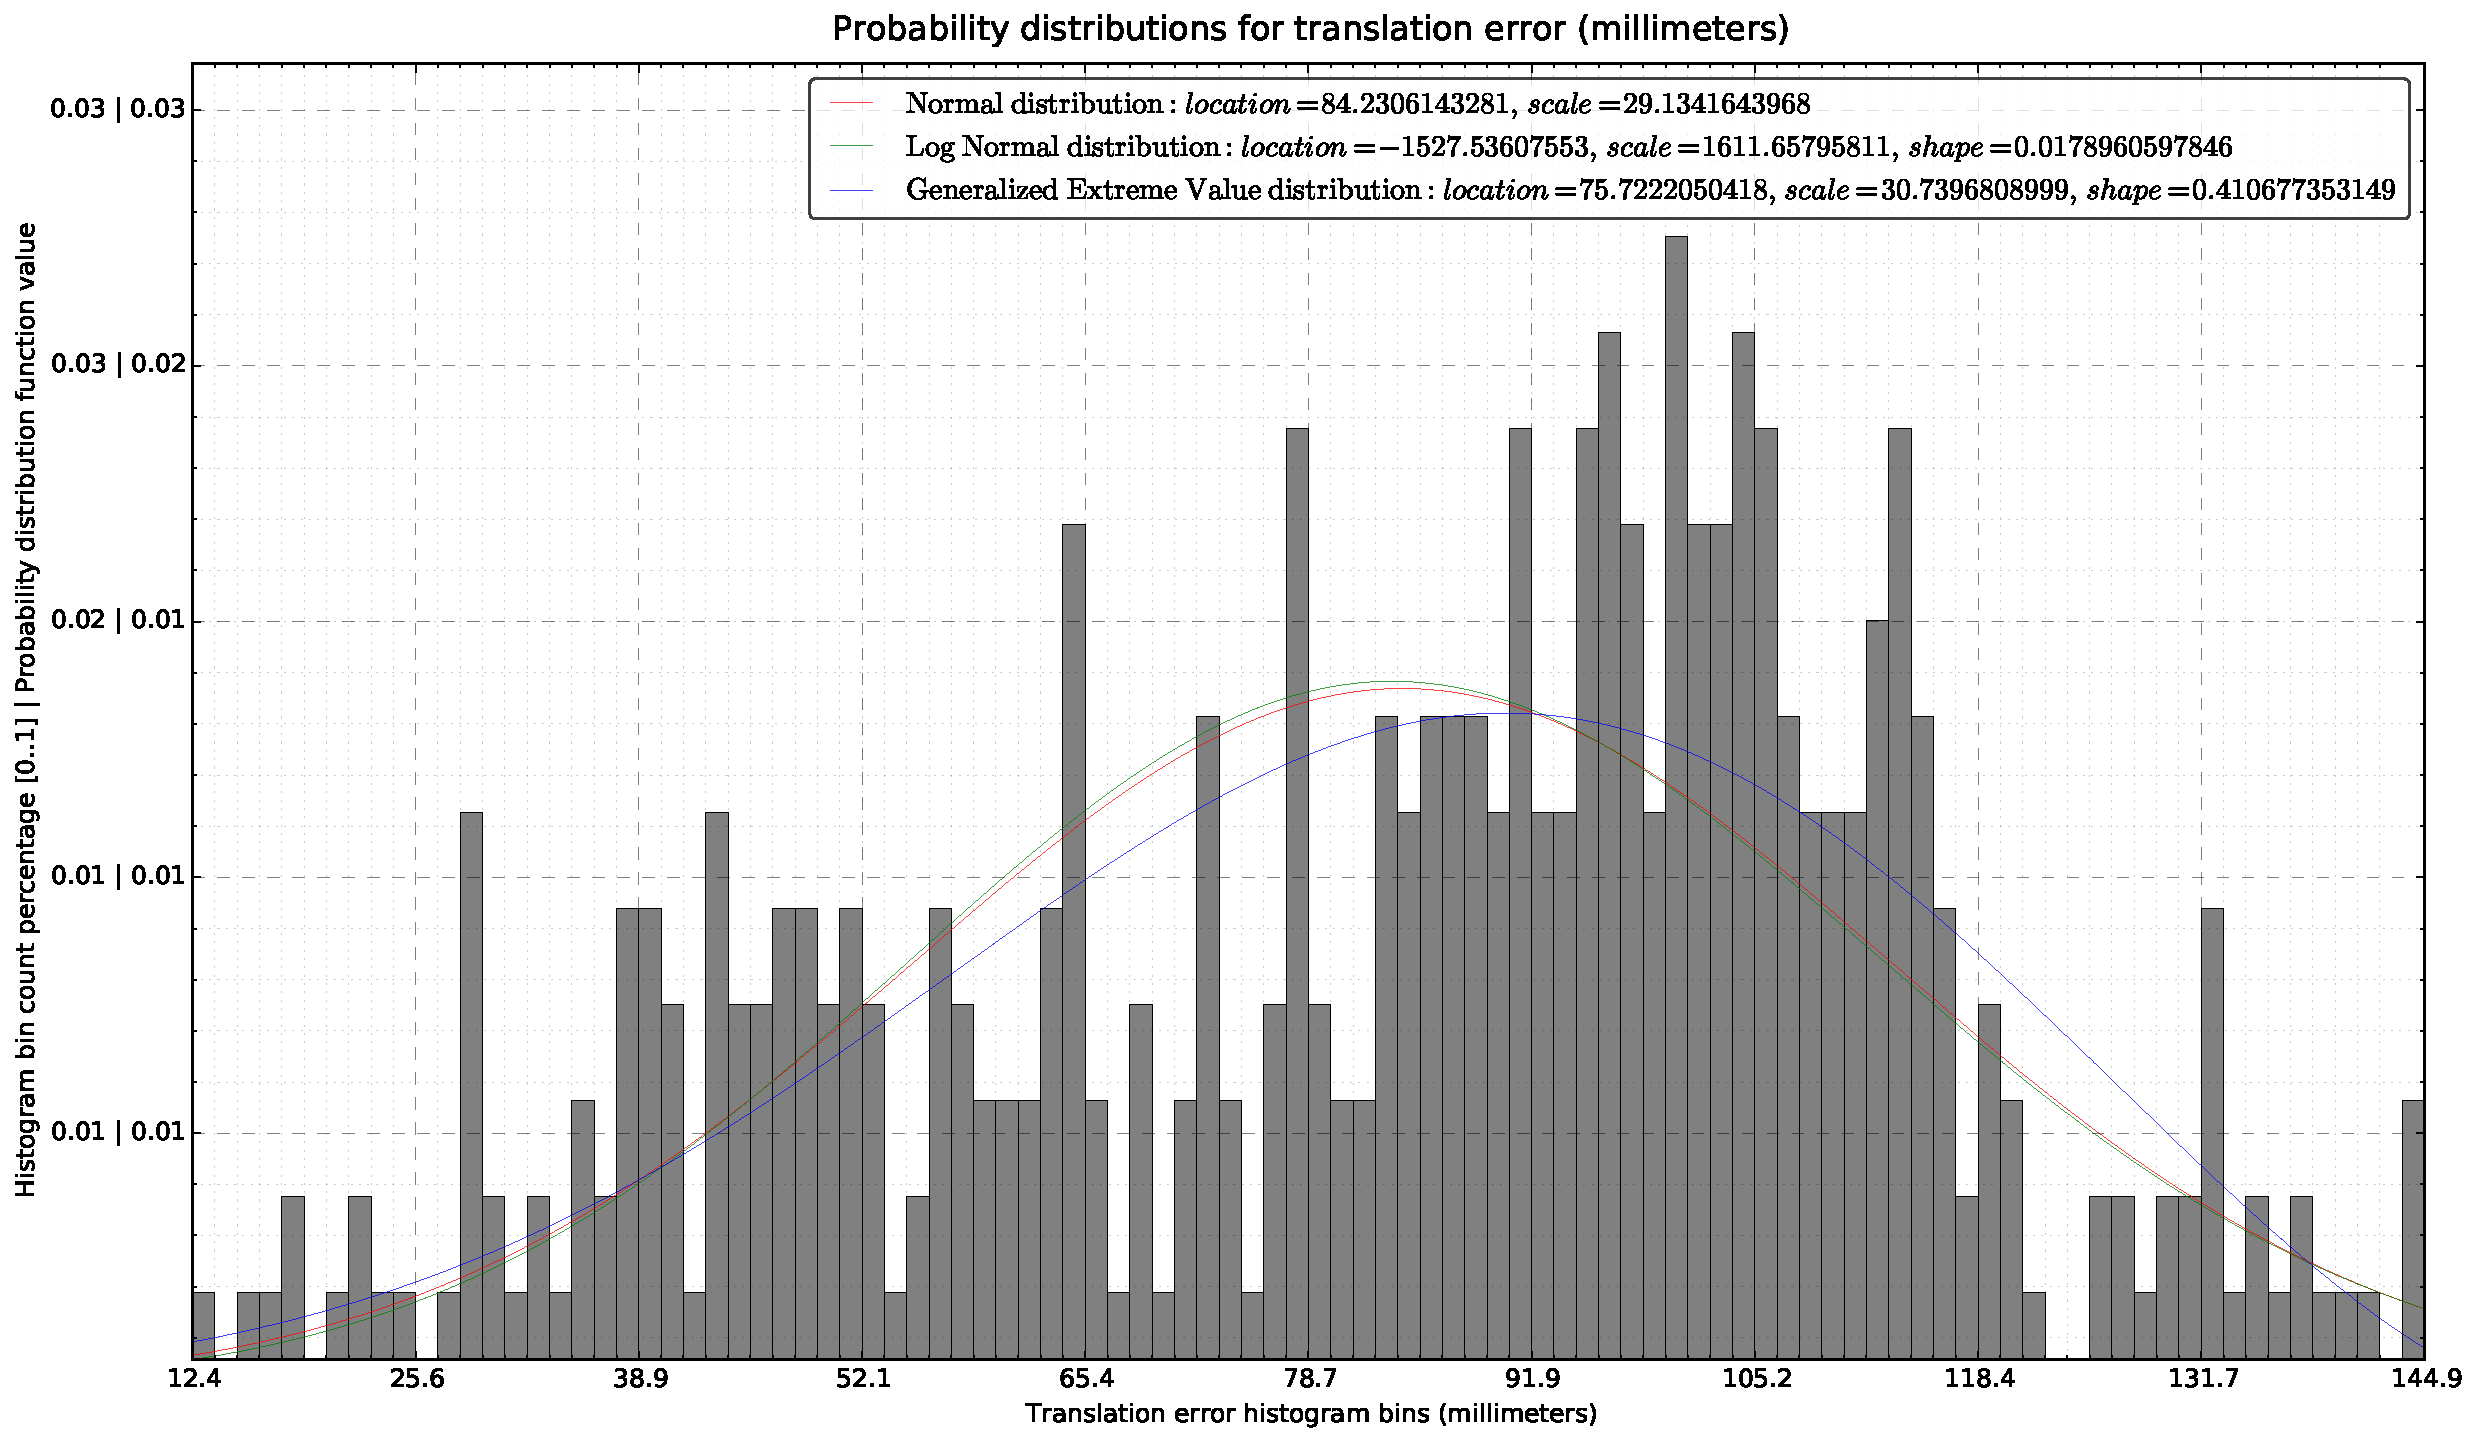
\includegraphics[trim={0 0 0 1cm}, clip, width=0.97\textwidth]{localization-system-evaluation/tests-3dof/jarvis-robot/complex-outliers-50-30-50-10-1-4-scans/graphs/translation-error-millimeters-distributions-amcl}
		\caption{Probability distributions for the \glsentrytext{amcl} translation errors}
		\label{fig:localization-system-evaluation_complex-path-with-outliers-50-30-50-10cm-per-sec-velocity-1-4-translation-error-amcl}
	\end{minipage}\hfill
	\begin{minipage}[H]{0.49\textwidth}
		\centering
		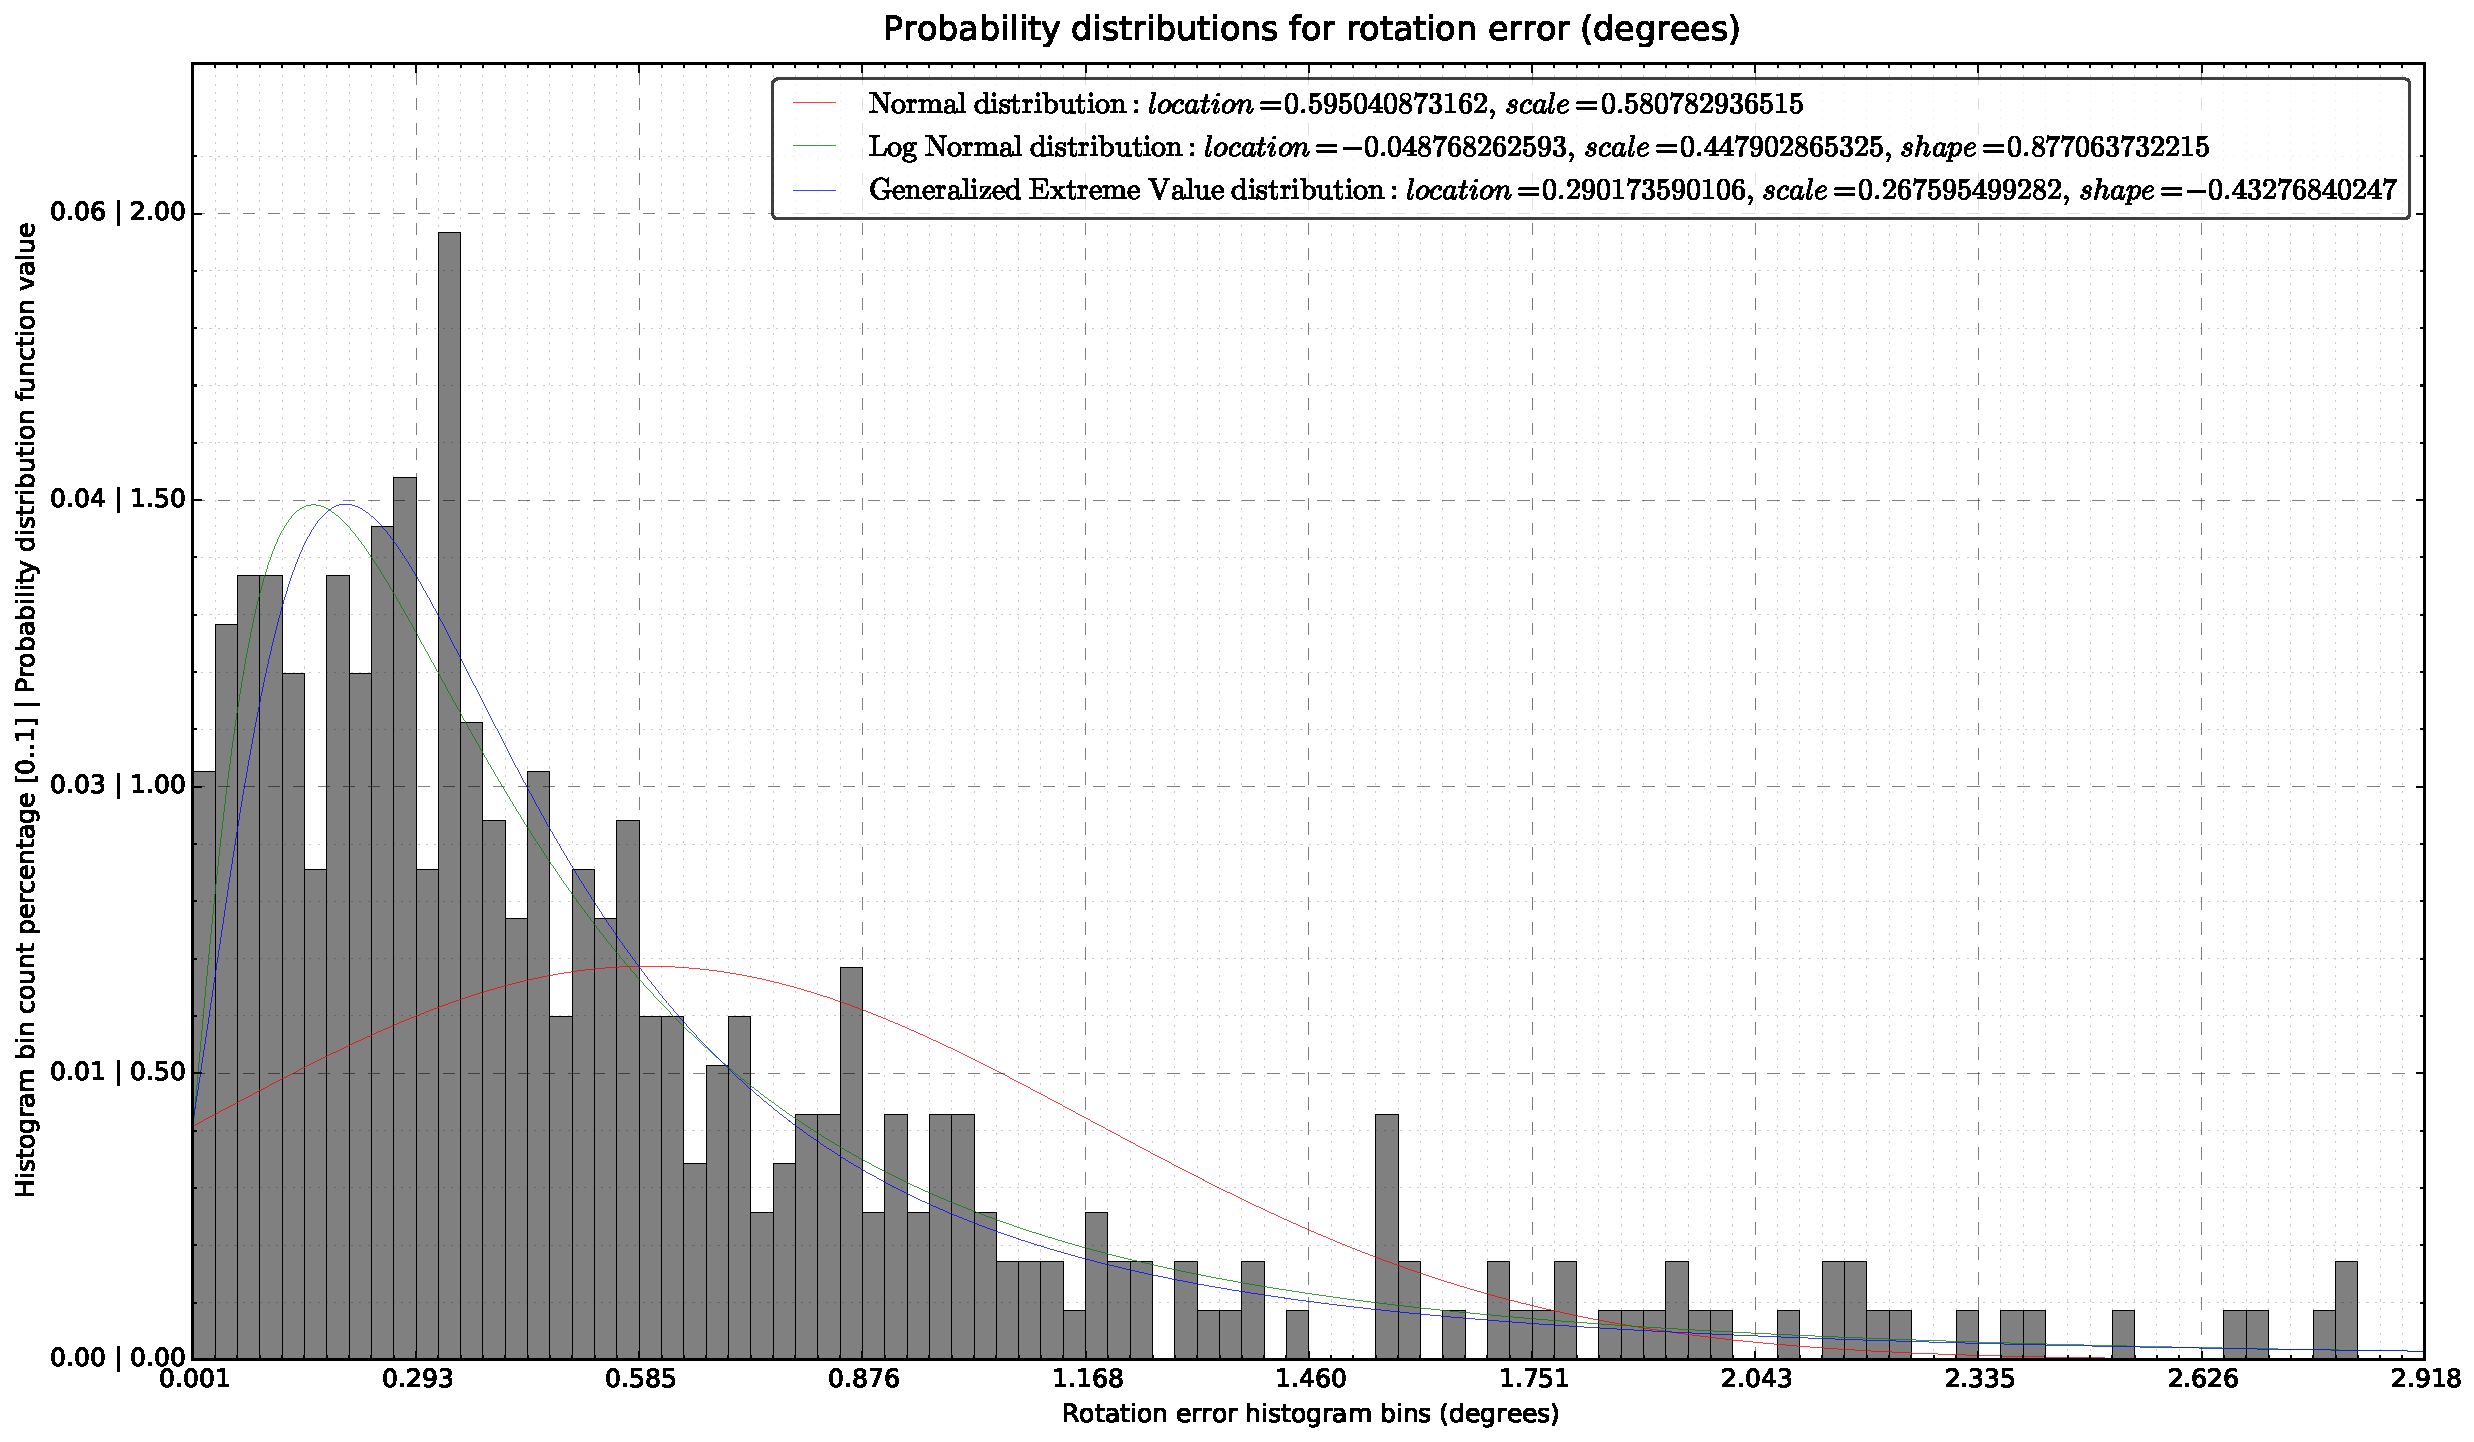
\includegraphics[trim={0 0 0 1cm}, clip, width=0.97\textwidth]{localization-system-evaluation/tests-3dof/jarvis-robot/complex-outliers-50-30-50-10-1-4-scans/graphs/rotation-error-degrees-distributions-amcl}
		\caption{Probability distributions for the \glsentrytext{amcl} rotation errors}
		\label{fig:localization-system-evaluation_complex-path-with-outliers-50-30-50-10cm-per-sec-velocity-1-4-rotation-error-amcl}
	\end{minipage}
\end{figure}

\begin{figure}[H]
	\centering
	\begin{minipage}[H]{0.49\textwidth}
		\centering
		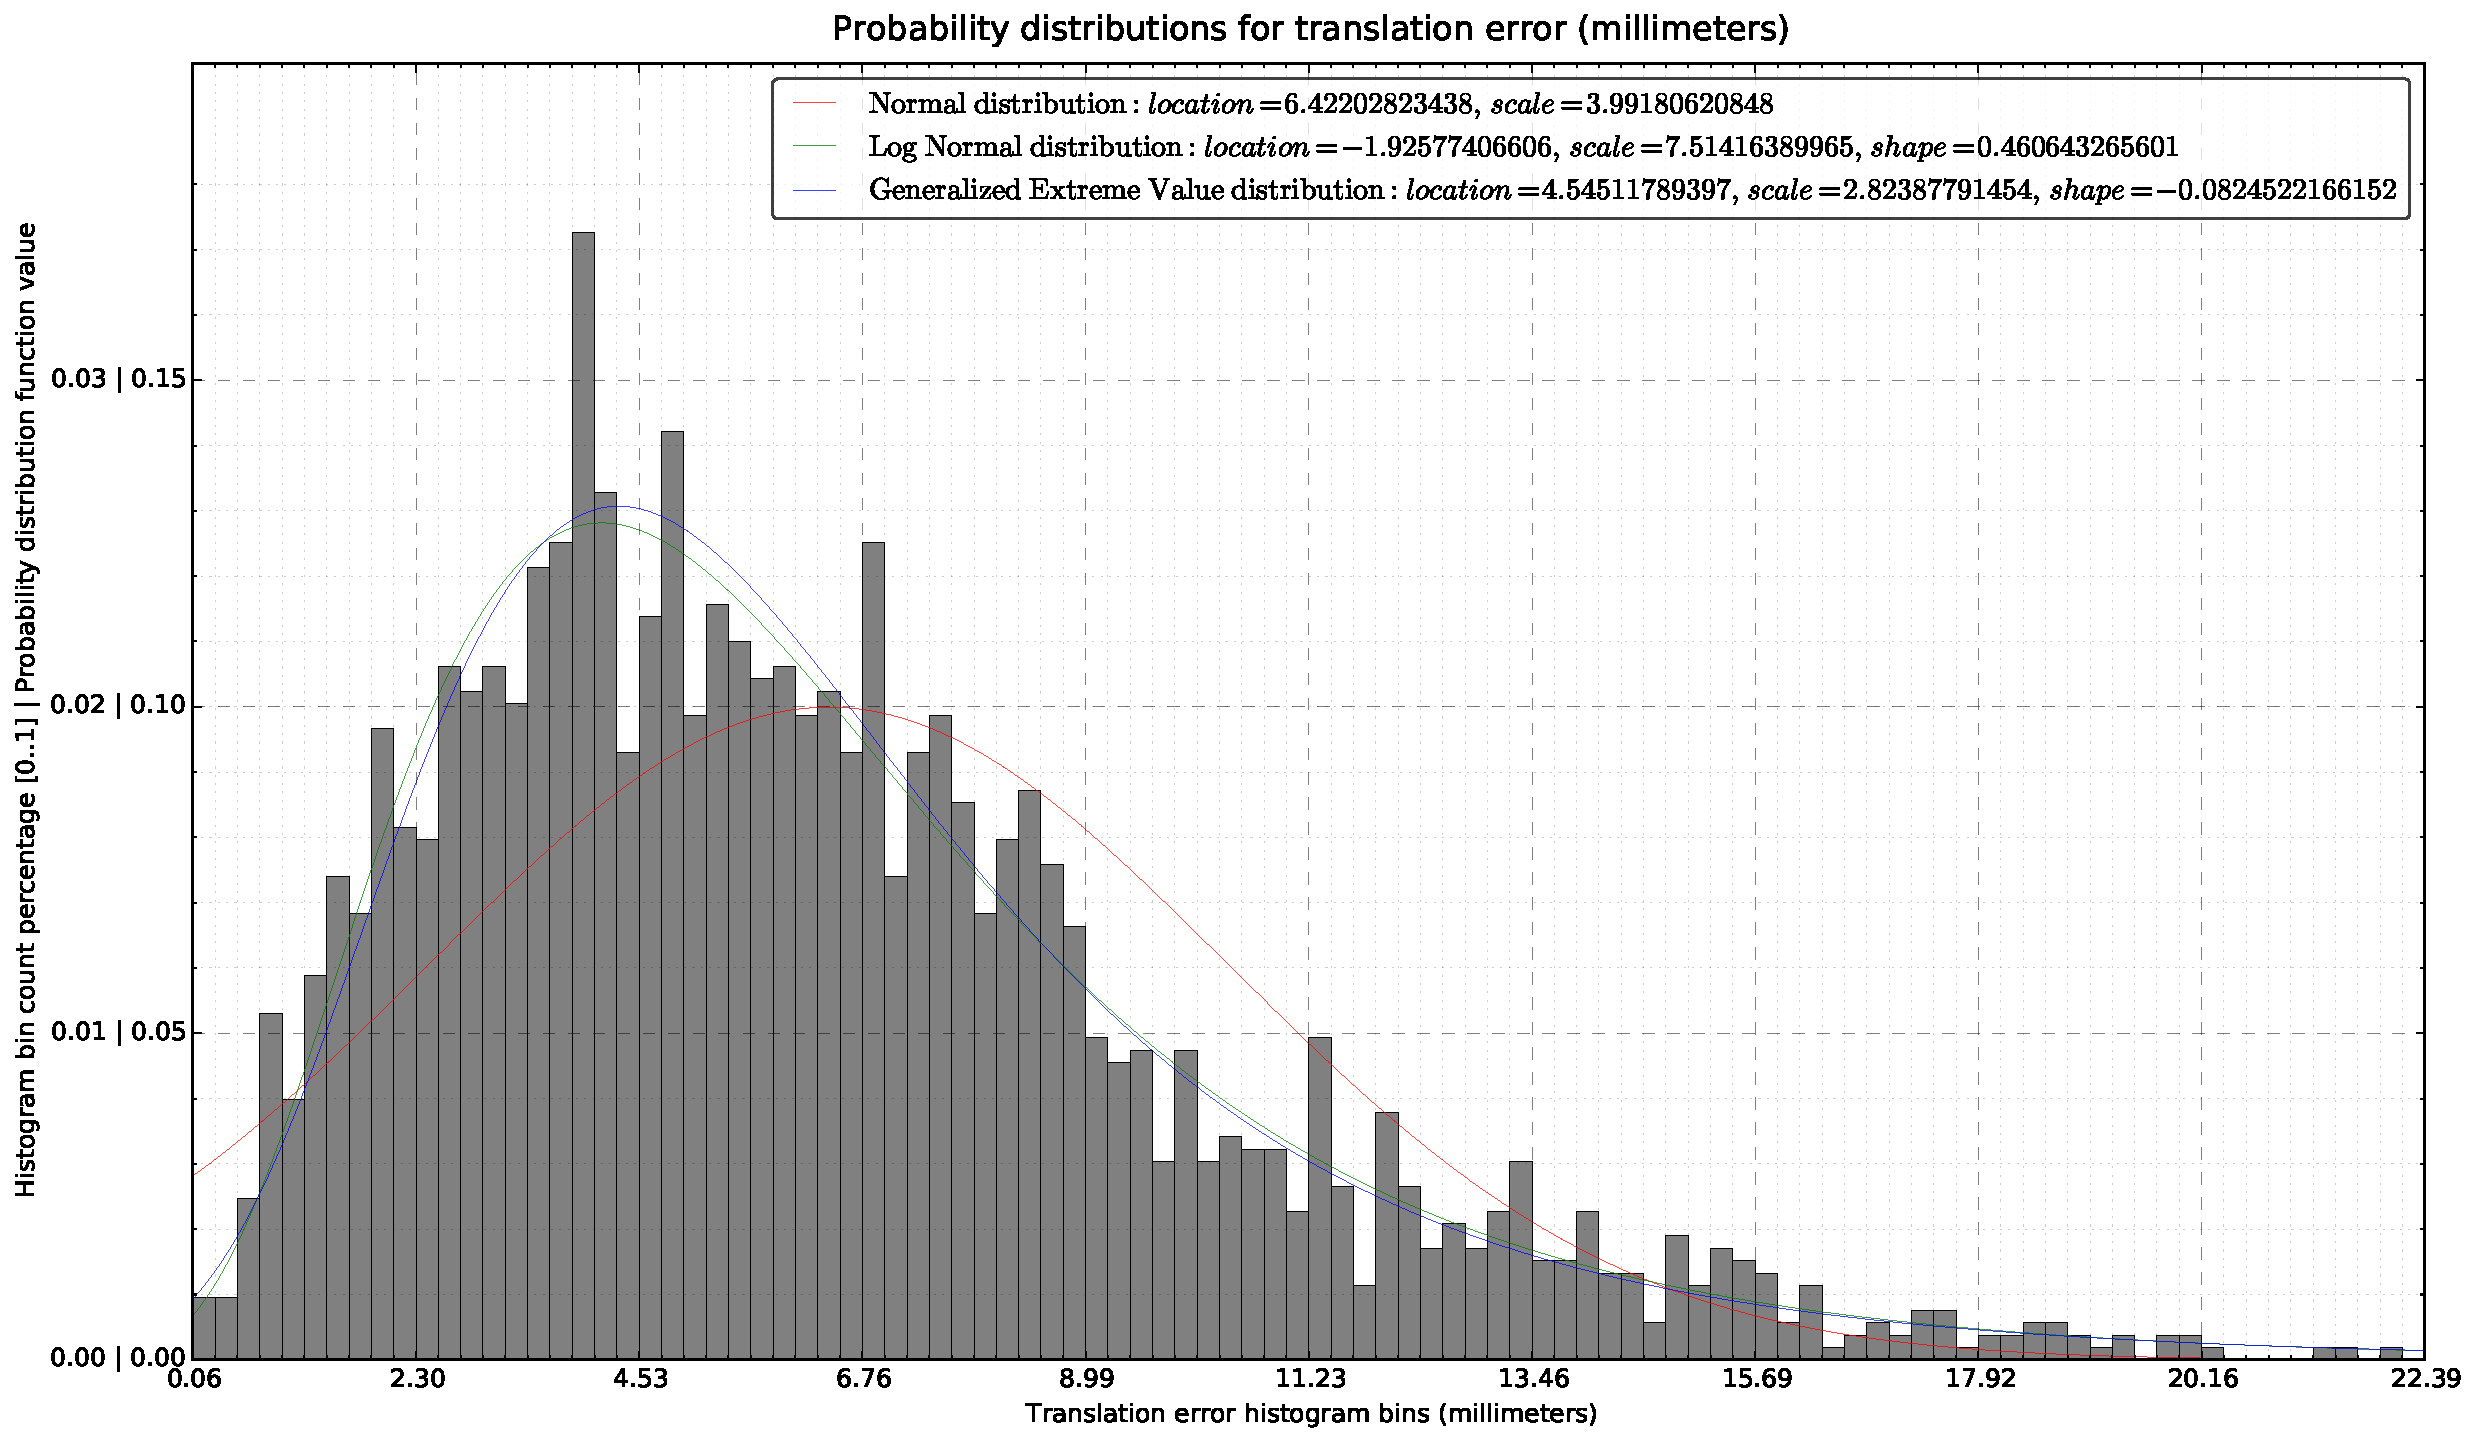
\includegraphics[trim={0 0 0 1cm}, clip, width=0.97\textwidth]{localization-system-evaluation/tests-3dof/jarvis-robot/complex-outliers-50-30-50-10-1-4-scans/graphs/translation-error-millimeters-distributions}
		\caption{Probability distributions for the localization system translation errors}
		\label{fig:localization-system-evaluation_complex-path-with-outliers-50-30-50-10cm-per-sec-velocity-1-4-translation-error}
	\end{minipage}\hfill
	\begin{minipage}[H]{0.49\textwidth}
		\centering
		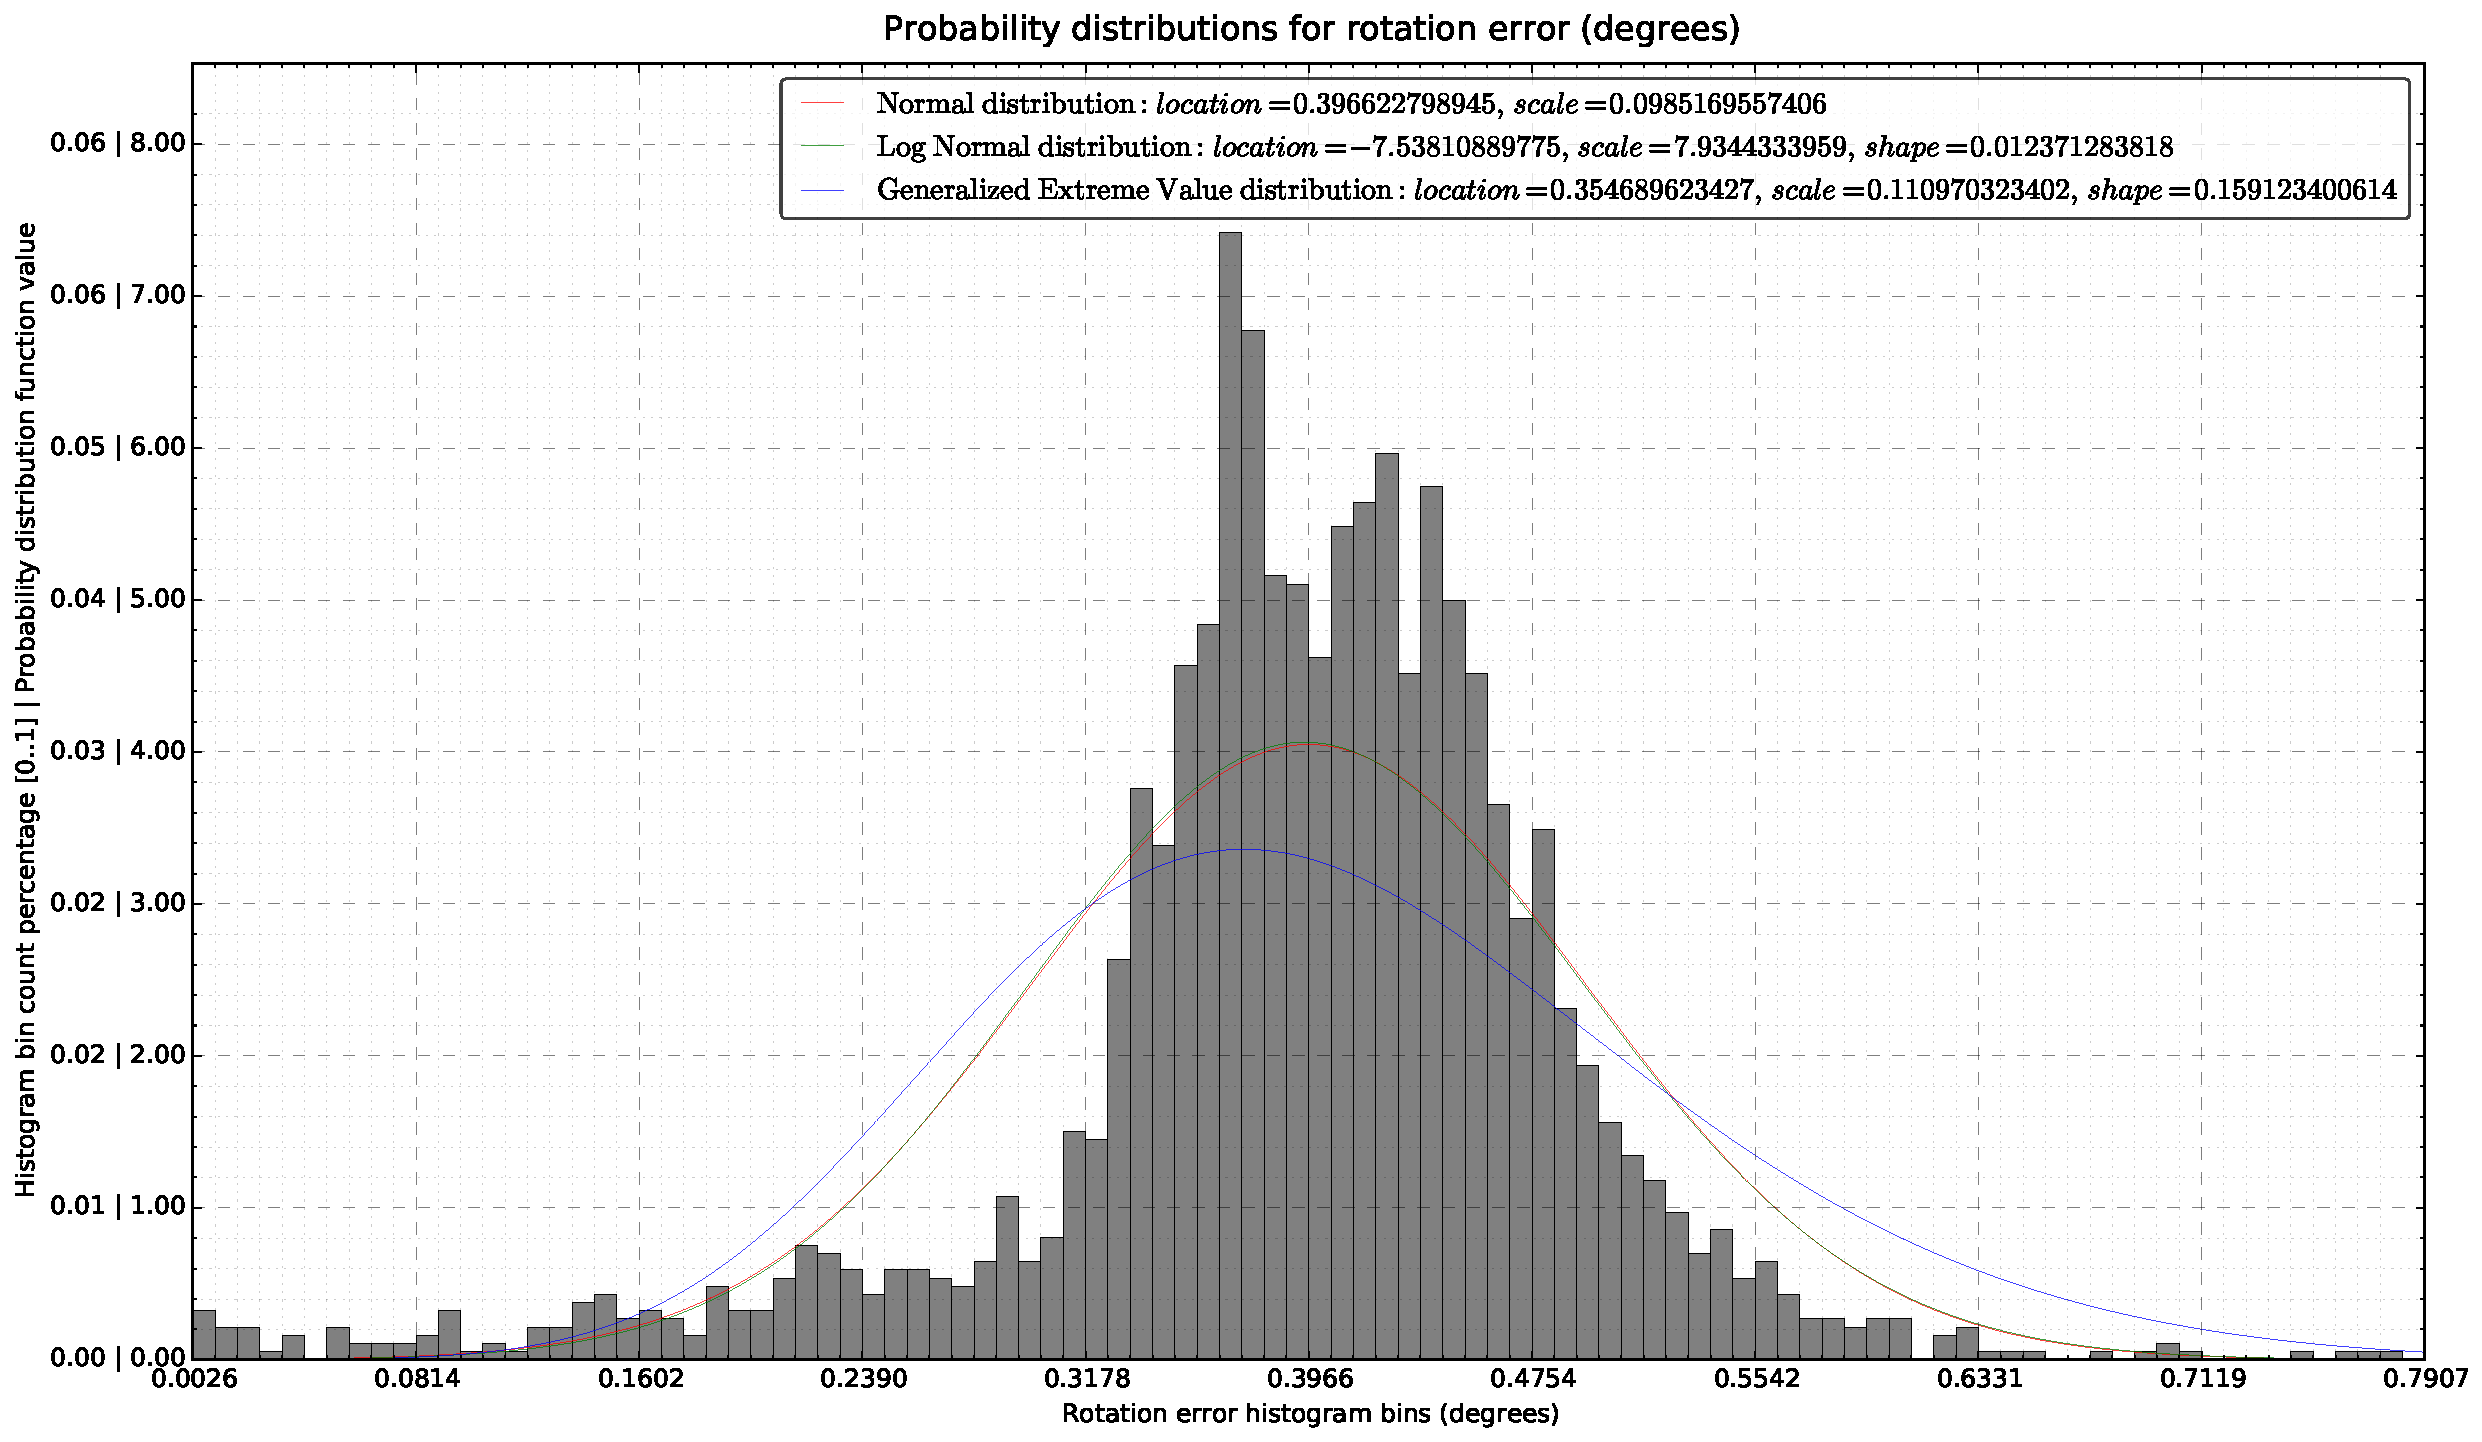
\includegraphics[trim={0 0 0 1cm}, clip, width=0.97\textwidth]{localization-system-evaluation/tests-3dof/jarvis-robot/complex-outliers-50-30-50-10-1-4-scans/graphs/rotation-error-degrees-distributions}
		\caption{Probability distributions for the localization system rotation errors}
		\label{fig:localization-system-evaluation_complex-path-with-outliers-50-30-50-10cm-per-sec-velocity-1-4-rotation-error}
	\end{minipage}
\end{figure}



\subsection{Computation time}

Looking at the computation time graphs in \Cref{tab:localization-system-evaluation_3-dof-results} and to \Cref{fig:localization-system-evaluation_complex-path-with-outliers-50-30-50-10cm-per-sec-velocity-1-4-scans-computation-time} it can be seen that the localization system can register the point clouds very fast (between 5 and 30 milliseconds), which is low enough to process all the incoming laser scans in real time (typically \glspl{lidar} generate scans every 100 milliseconds). Moreover, the computation time seems to be very stable, with occasional peaks due to laser deformation or varying percentage of outliers.

The global computation time is mostly associated with the point cloud registration stage, while the rest of it is due to normal estimation and point cloud preprocessing algorithms.

\begin{figure}[H]
	\centering
	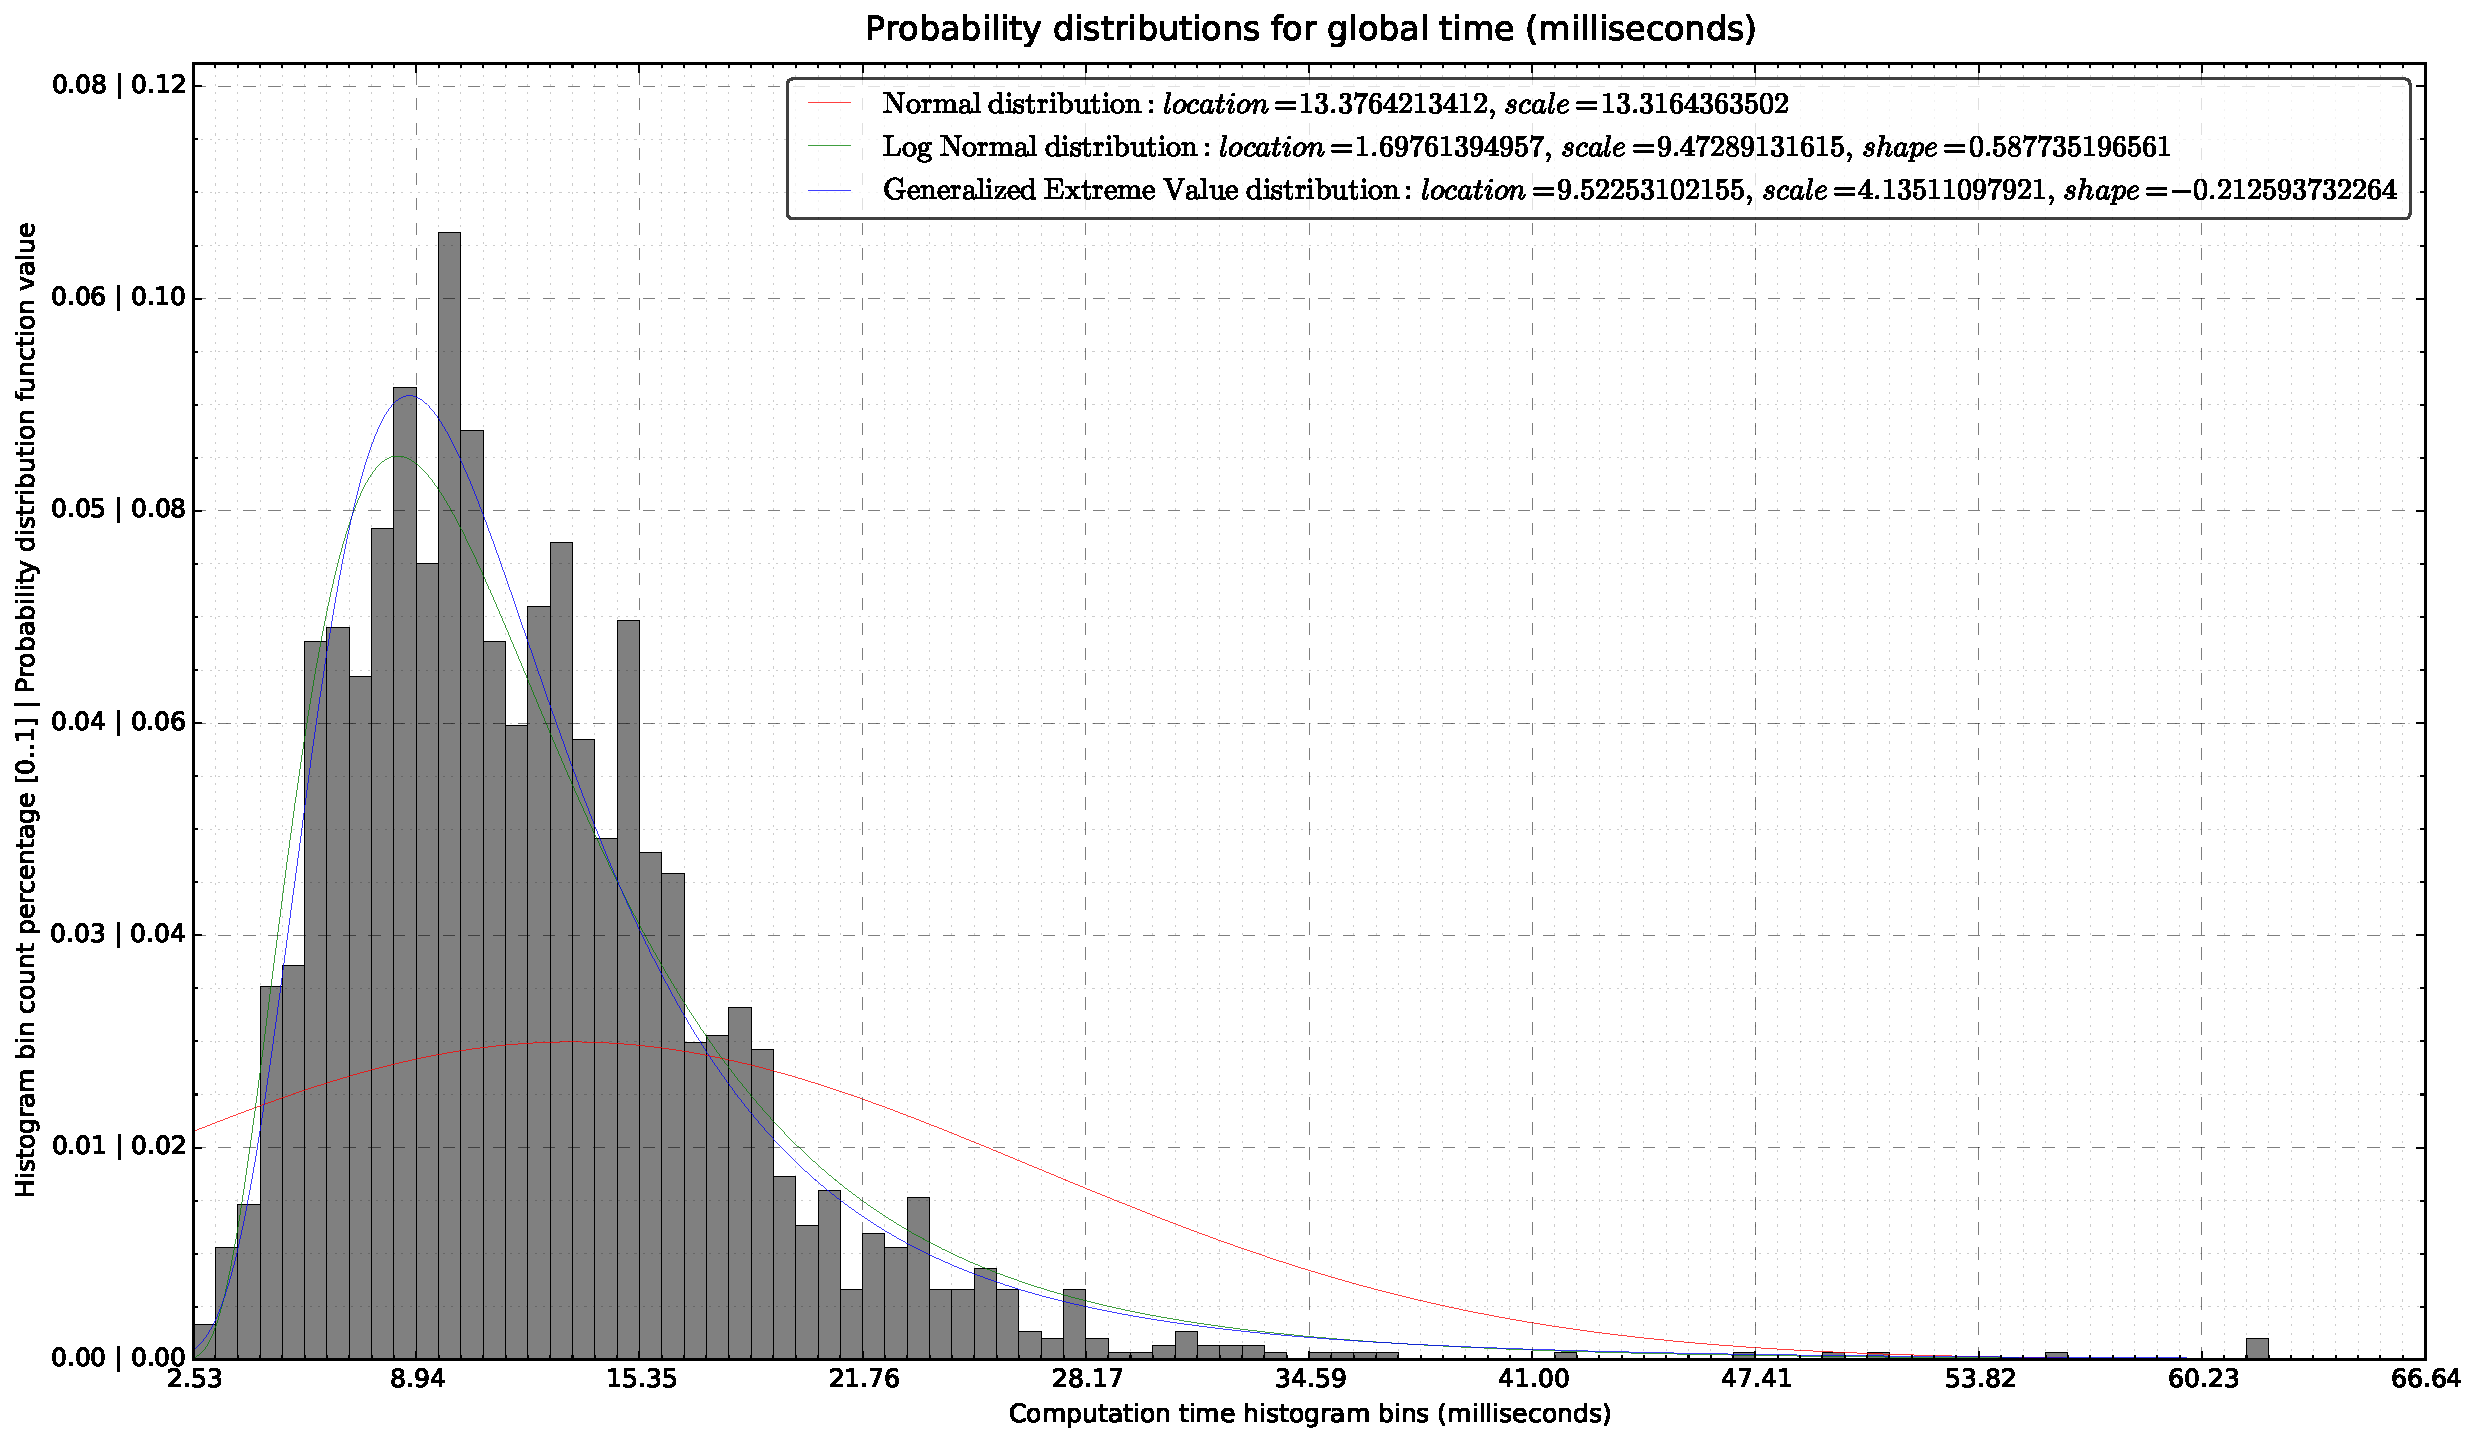
\includegraphics[trim={0 0 0 1cm}, clip, width=0.49\textwidth]{localization-system-evaluation/tests-3dof/jarvis-robot/complex-outliers-50-30-50-10-1-4-scans/graphs/computation-times-milliseconds-global-time-distributions}
	\caption{Probability distributions for the localization system global computation time}
	\label{fig:localization-system-evaluation_complex-path-with-outliers-50-30-50-10cm-per-sec-velocity-1-4-scans-computation-time}
\end{figure}


\subsection{Mapping}

Any self-localization system requires a map to estimate the pose of the robot when using exteroceptive information. If such map doesn't exist, then the first live point cloud can be considered as the initial map, and then it can be updated dynamically as new sensor data is processed.

The dynamic and incremental map update capability of the \gls{drl} system can be used to register the full sensor point clouds or only the inliers / outliers. Full integration is useful when starting a map from scratch (example in \Cref{fig:localization-system-evaluation_drl-2.5cm-1.0-bag-speed}). Partial integration can be useful when there is a highly detailed map (for example generated from a \gls{cad} model or with other high accuracy mapping system) and we only want to add or remove information from it, such as integrating new large objects and opening doors in the map (examples from \crefrange{fig:localization-system-evaluation_indoor-10mm}{fig:localization-system-evaluation_indoor-10mm-mapping-partial-integration}). Partial integration besides reducing the computational resources required it also allows to keep the detail of the original map (by avoiding deformations due to sensor measurement noise). This can be clearly seen in \Cref{fig:localization-system-evaluation_lab-10mm-dynamic} in which the sensor noise polluted the walls of the original map (given that the map cell resolution was much smaller than the mean sensor noise). By performing selective mapping this problem was avoided in the map present in \Cref{fig:localization-system-evaluation_indoor-10mm-dynamic} (by inserting on the map only unknown zones while keeping the walls generated from the \gls{cad} model untouched).

Looking at planar structures from \crefrange{fig:localization-system-evaluation_drl-2.5cm-1.0-bag-speed}{fig:localization-system-evaluation_gmapping-2.5cm-1.0-bag-speed} it can be seen that the \gls{drl} system was able to achieve equal or even better mapping results than the GMapping\footnote{\url{http://wiki.ros.org/gmapping}} \gls{slam} system and even the ground truth provided by the Raptor-E cameras (that seems to be less suitable for mapping than both the \gls{drl} system and the GMapping \gls{ros} package).

\begin{figure}[H]
	\centering
	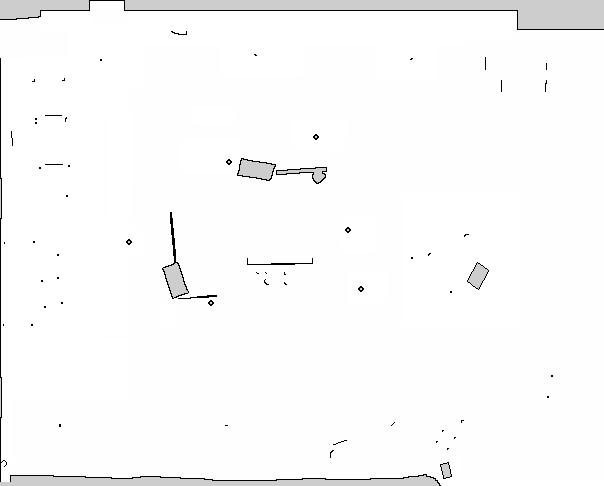
\includegraphics[width=0.43\textwidth]{localization-system-evaluation/tests-3dof/maps/industrial-hall/drl-corrected}
	\caption{Map manually corrected with 25 mm cell resolution (based on \Cref{fig:localization-system-evaluation_drl-2.5cm-1.0-bag-speed}) }
	\label{fig:localization-system-evaluation_drl-corrected}
\end{figure}

\begin{figure}[H]
	\centering
	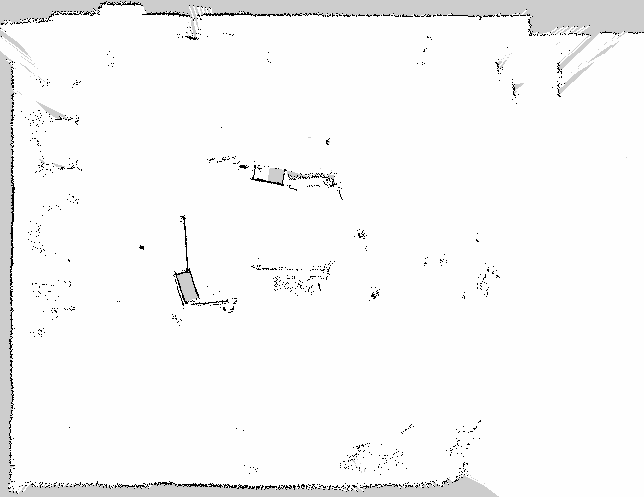
\includegraphics[width=0.45\textwidth]{localization-system-evaluation/tests-3dof/maps/industrial-hall/drl-2.5cm-1.0-bag-speed}
	\caption{Map made with the localization system using full integration in conjunction with OctoMap}
	\label{fig:localization-system-evaluation_drl-2.5cm-1.0-bag-speed}
\end{figure}


\begin{figure}[H]
	\centering
	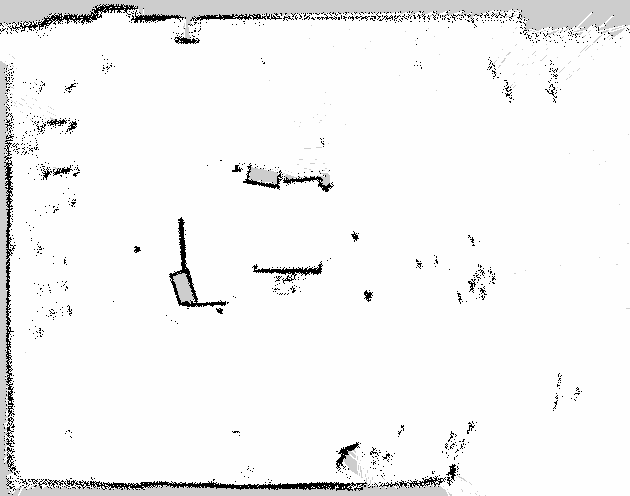
\includegraphics[width=0.45\textwidth]{localization-system-evaluation/tests-3dof/maps/industrial-hall/ground-truth-2.5cm-0.245-time-offset}
	\caption{Map made using the ground truth poses provided by the Raptor-E cameras}
	\label{fig:localization-system-evaluation_ground-truth-2.5cm-0.245-time-offset}
\end{figure}


\begin{figure}[H]
	\centering
	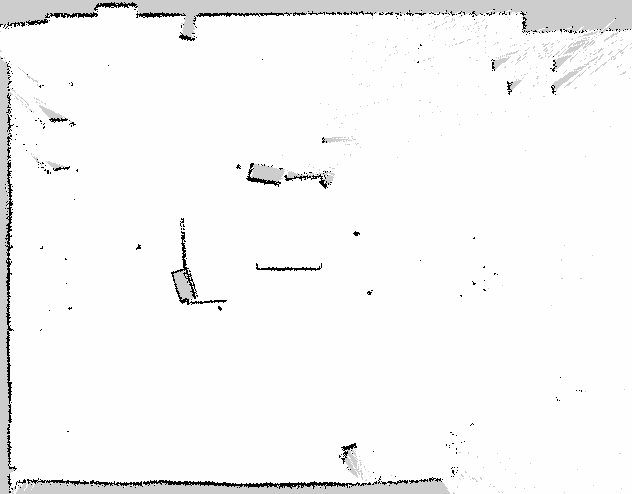
\includegraphics[width=0.45\textwidth]{localization-system-evaluation/tests-3dof/maps/industrial-hall/gmapping-2.5cm-0.1-bag-speed}
	\caption{Map made with the GMapping package playing the rosbag at 10\% speed}
	\label{fig:localization-system-evaluation_gmapping-2.5cm-0.1-bag-speed}
\end{figure}

\begin{figure}[H]
	\centering
	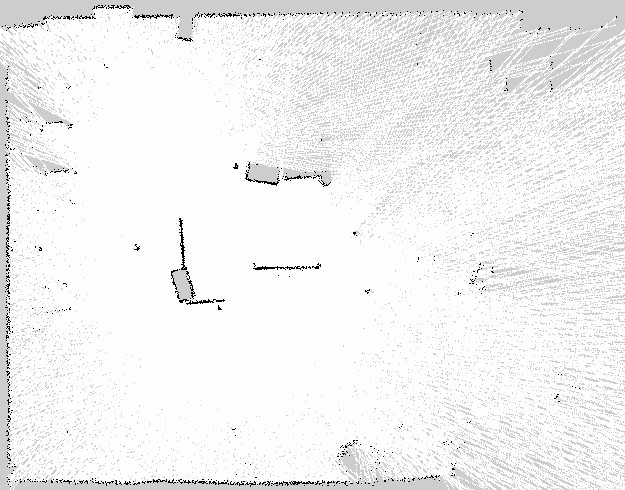
\includegraphics[width=0.45\textwidth]{localization-system-evaluation/tests-3dof/maps/industrial-hall/gmapping-2.5cm-1.0-bag-speed}
	\caption{Map made with the GMapping package playing the rosbag in real time}
	\label{fig:localization-system-evaluation_gmapping-2.5cm-1.0-bag-speed}
\end{figure}


\begin{figure}[H]
	\centering
	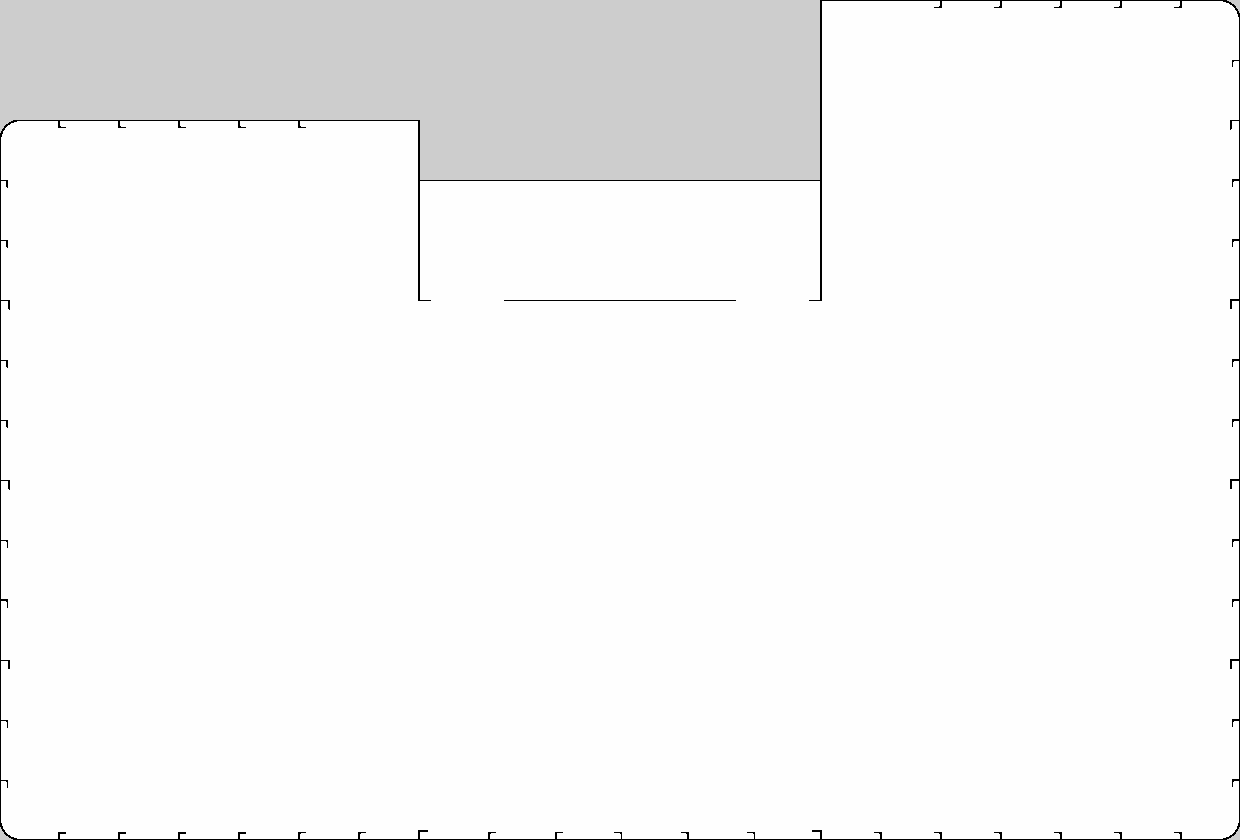
\includegraphics[width=0.45\textwidth]{localization-system-evaluation/tests-3dof/maps/indoor-10mm}
	\caption{Map of structured environment generated using a CAD model}
	\label{fig:localization-system-evaluation_indoor-10mm}
\end{figure}

\begin{figure}[H]
	\centering
	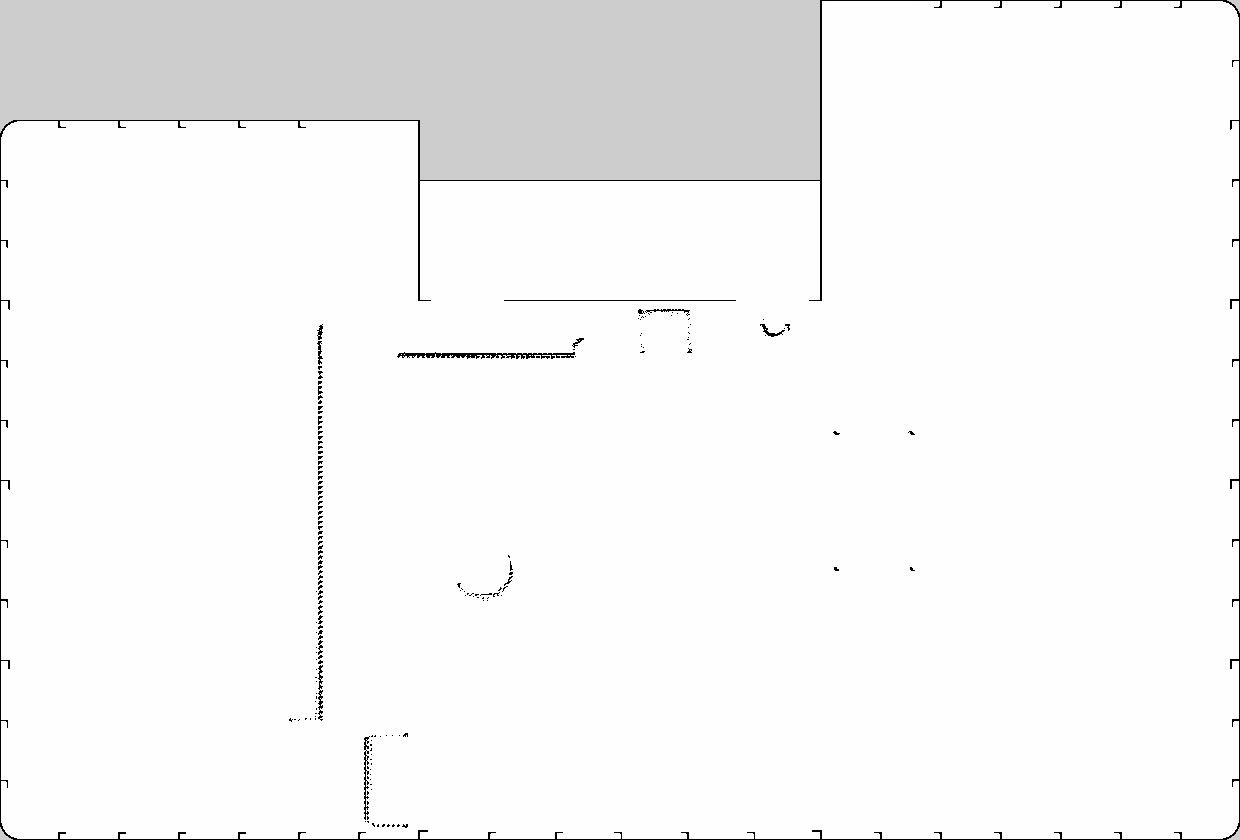
\includegraphics[width=0.45\textwidth]{localization-system-evaluation/tests-3dof/maps/indoor-10mm-mapping-partial-integration}
	\caption{Updated map of structured environment using partial integration (only points that were not close to the walls were integrated)}
	\label{fig:localization-system-evaluation_indoor-10mm-mapping-partial-integration}
\end{figure}

\begin{figure}[H]
	\centering
	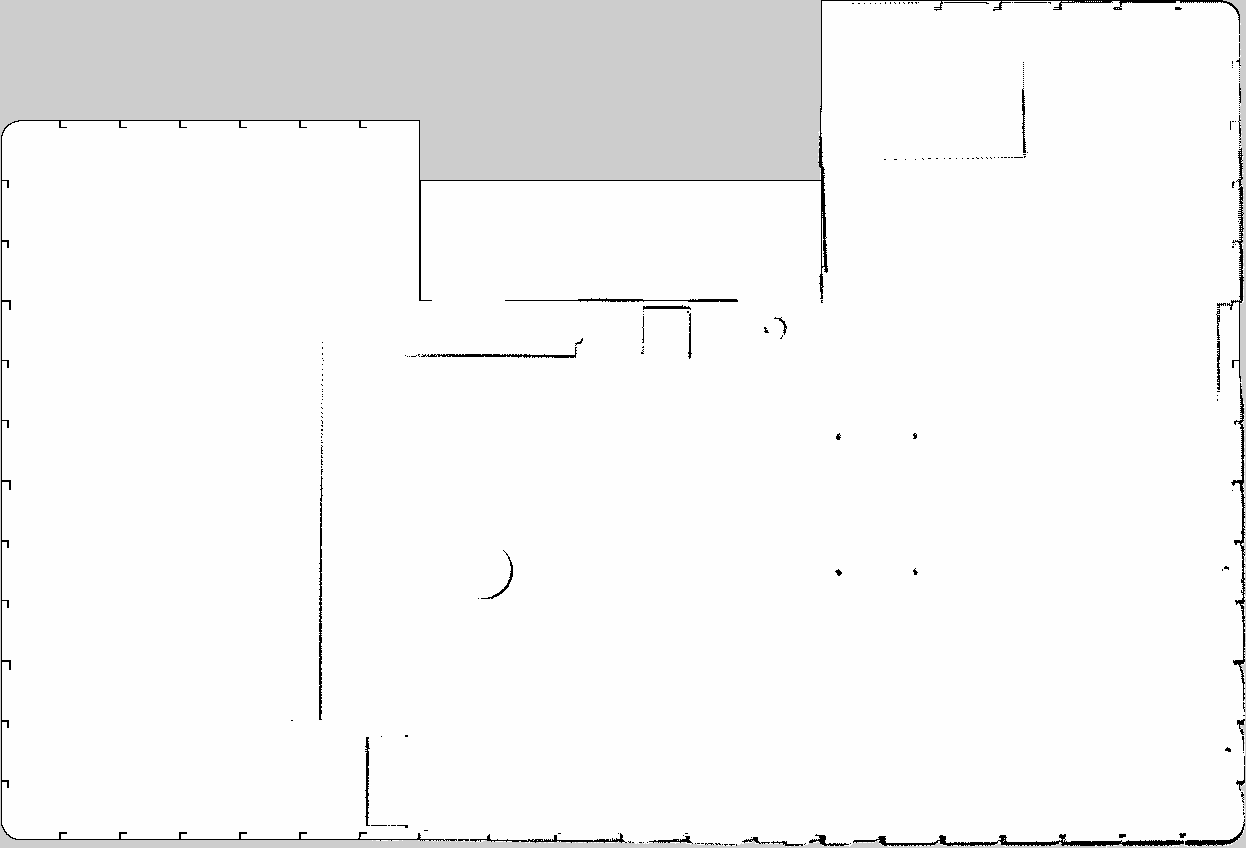
\includegraphics[width=0.45\textwidth]{localization-system-evaluation/tests-3dof/maps/indoor-10mm-mapping-full-integration}
	\caption{Updated map of structured environment using full integration (all registered were integrated)}
	\label{fig:localization-system-evaluation_indoor-10mm-mapping-full-integration}
\end{figure}

\begin{figure}[H]
	\centering
	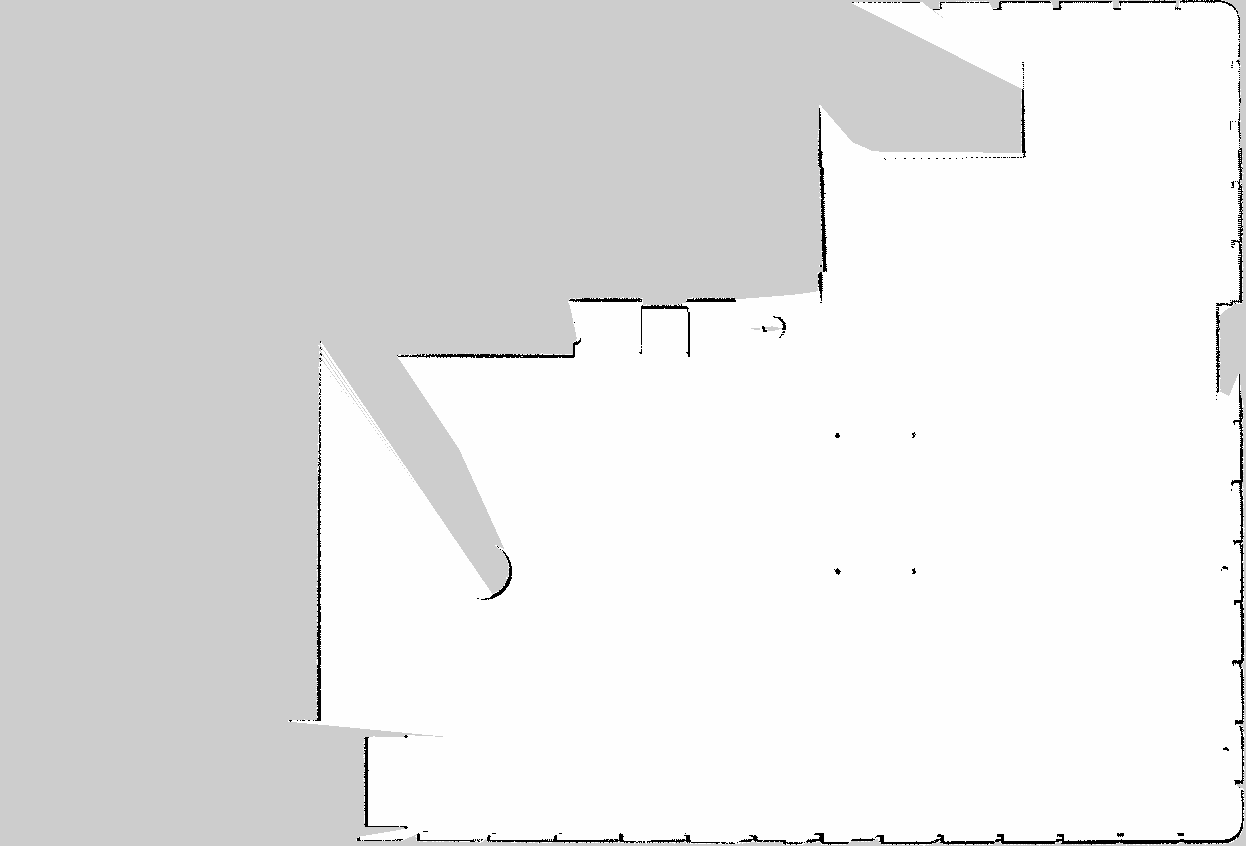
\includegraphics[width=0.45\textwidth]{localization-system-evaluation/tests-3dof/maps/indoor-10mm-mapping}
	\caption{Mapping of the structured environment using full integration (all registered were integrated)}
	\label{fig:localization-system-evaluation_indoor-10mm-mapping}
\end{figure}

\begin{figure}[H]
	\centering
	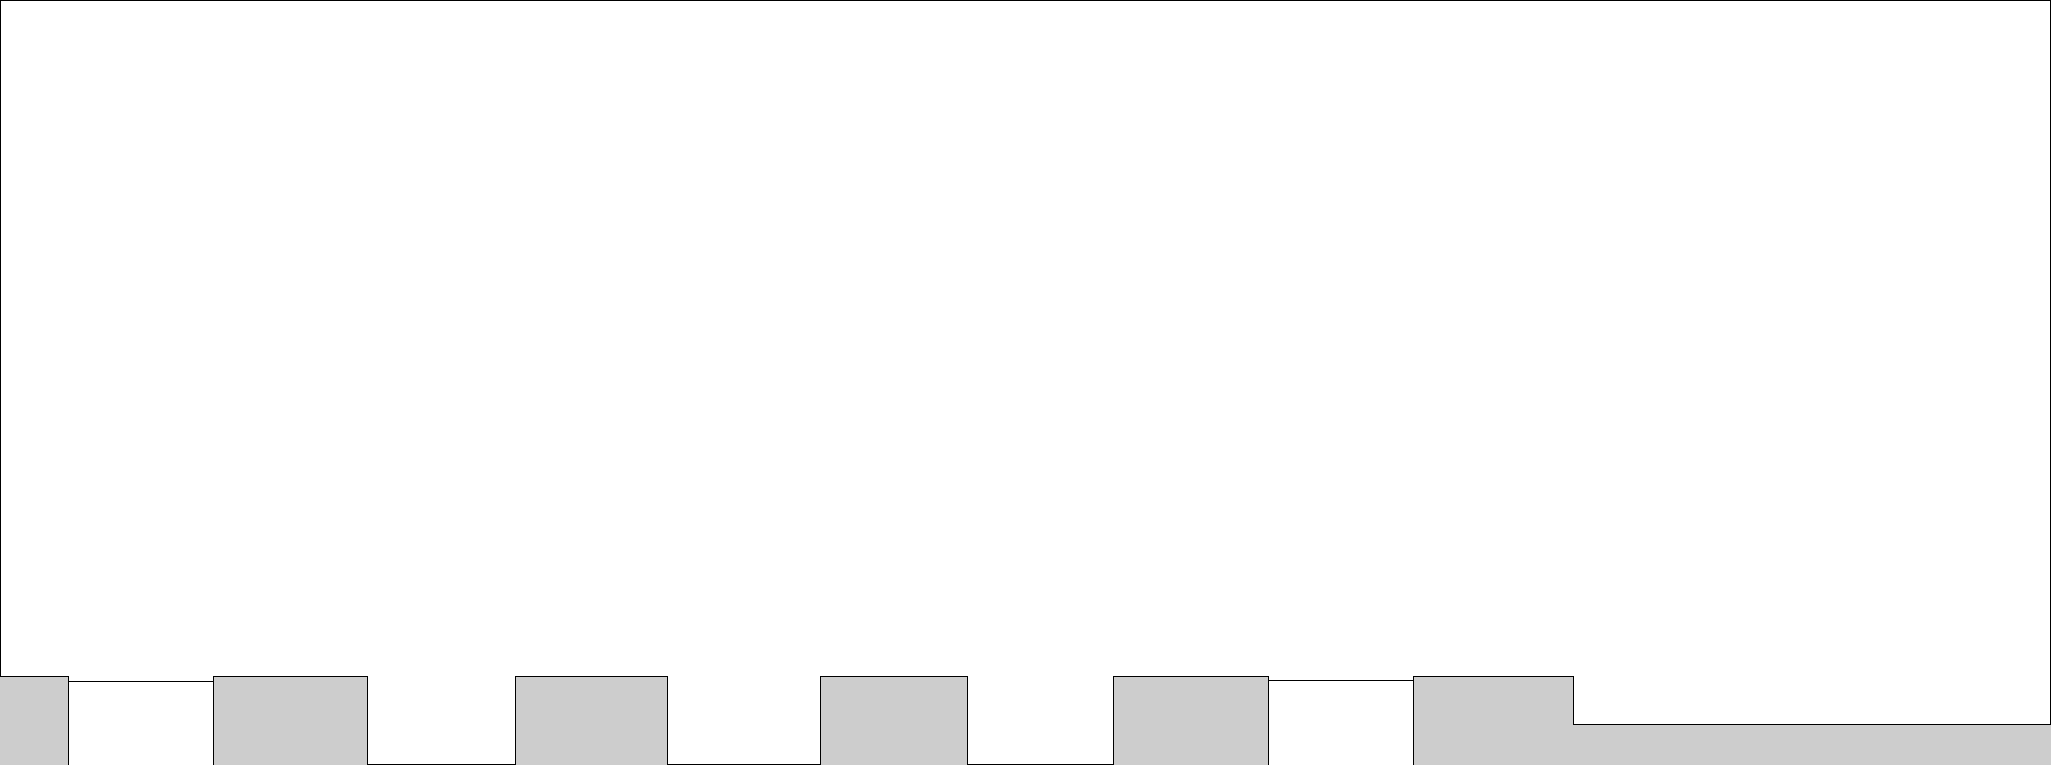
\includegraphics[width=0.45\textwidth]{localization-system-evaluation/tests-3dof/maps/lab-10mm}
	\caption{RoboCup field map (manually corrected)}
	\label{fig:localization-system-evaluation_lab-10mm}
\end{figure}

\begin{figure}[H]
	\centering
	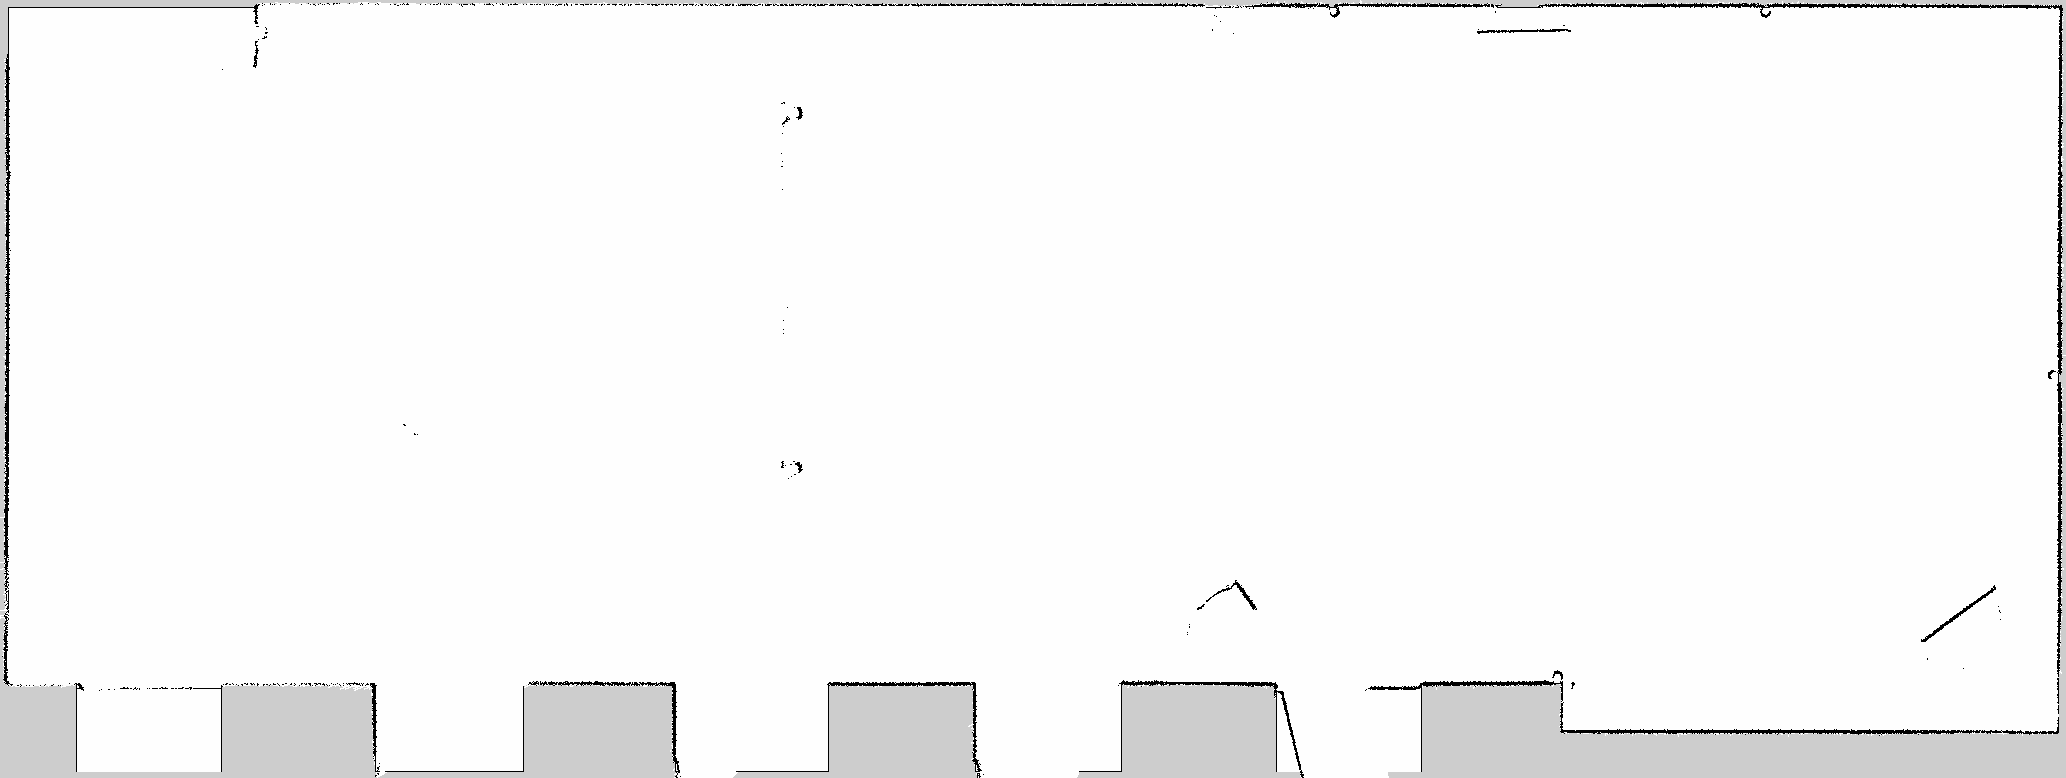
\includegraphics[width=0.45\textwidth]{localization-system-evaluation/tests-3dof/maps/lab-10mm-dynamic}
	\caption{Updated map of RoboCup field using full integration (starting with the map from \Cref{fig:localization-system-evaluation_lab-10mm})}
	\label{fig:localization-system-evaluation_lab-10mm-dynamic}
\end{figure}



%\clearpage

\section{6 \glsentrytext{dof} localization system tests}\label{sec:tridimensional-localization-system-tests}

\subsection{Overview}

The main 6 \gls{dof} results retrieved with the localization system are shown in \Cref{tab:localization-system-evaluation_6-dof-results}. The first two experiments (fly and translations movements) were performed to evaluate the accuracy of the point cloud registration algorithms while the last one (mainly rotation movements) aimed to test the robustness against temporary absence of valid sensor data (in this test the Kinect had periods in which most of its field of view was outside the map).

These tests were retrieved with a known initial pose and used \gls{icp} point-to-point as tracking algorithm and \gls{icp} point-to-plane as tracking recovery method. The tests with the ethzasl\_icp\_mapper used the \gls{icp} point-to-plane since the implementation of the \gls{icp} point-to-point was consistently losing tracking (the authors of this systems also point out in \cite{Pomerleau2013a} that \gls{icp} point-to-plane implementation was more robust and achieved more accurate tracking).

The 3D map was done with the localization system in \gls{slam} mode and used continuous surface reconstruction in order to create an accurate representation of the environment and reduce the impact of the measurements noise. This map was later downsampled using a voxel grid with 20 mm cells in order to allow real-time processing of the Kinect data.

The next sections will provide an analysis of the 6 \gls{dof} results achieved with the \gls{drl} system. It will start by explaining the importance of point cloud processing and how it helps reduce the cloud registration time. Then it will give an overview of the 3D map building capabilities and it will finish with an analysis of the translation and rotation errors along with the computation time.


\begin{sidewaystable}
	\caption{6 \glsentrytext{dof} results}
	\tabulinesep = 1.2ex
	\setlength{\tabcolsep}{0.2em}
	\centering
	\scriptsize
	\begin{tabu} to \textwidth { X[m,c] X[m,c] X[m,c] X[1.7m,c] X[0.01m,c] X[m,c] X[m,c] X[0.01m,c] X[m,c] X[m,c] X[0.01m,c] X[m,c] X[m,c] X[0.01m,c] X[m,c] X[m,c] X[0.01m,c] X[m,c] X[m,c] }
		\hline
		\multicolumn{4}{c}{Test conditions} 												&& \multicolumn{2}{c}{Translation error (mm)} && \multicolumn{2}{c}{Rotation error (degrees)} && \multicolumn{2}{c}{Outliers \% [0..100]} && \multicolumn{2}{c}{Processing time (ms)} && \multicolumn{2}{c}{Cloud registrations} \\
		\cline{1-4} \cline{6-7} \cline{9-10} \cline{12-13} \cline{15-16} \cline{18-19}
		Path shape 														& Path velocity 									& Map cell resolution 							& System				&& Mean   	& Standard deviation 	&& Mean  	& Standard deviation 	&& Mean  	& Standard deviation 	&& Mean     & Standard deviation	&& Success ratio & Tracking recovery ratio \\ \hline
		\multirow{2}{0.05\textwidth}{\centering Overview fly}			& \multirow{2}{0.05\textwidth}{\centering 30 cm/s}	& \multirow{6}{0.05\textwidth}{\centering 20 mm}& \gls{drl}				&& 17.926	&   9.789				&& 3.027 	& 0.638					&& 0.165	& 0.172					&&  30.714  & 	11.407				&& 473/501 		 & 0/501 	\\
																		&													&												& ethzasl\_icp\_mapper 	&& 22.810	&  17.579				&& 3.477	& 1.958					&& --		& --					&& 324.716  &  173.477				&& 180/501 		 & -- 		\\
		\multirow{2}{0.05\textwidth}{\centering Mainly translations}	& \multirow{2}{0.05\textwidth}{\centering 20 cm/s}	& 												& \gls{drl} 			&& 14.162	&   7.990				&& 2.486 	& 0.975					&& 0.983	& 1.874					&&  32.296  & 	10.757				&& 809/926 		 & 0/926 	\\
																		&													&												& ethzasl\_icp\_mapper 	&& 31.420	&  52.280				&& 2.915	& 0.637					&& --		& --					&& 292.265  &  167.868				&& 358/926 		 & -- 		\\
		\multirow{2}{0.05\textwidth}{\centering Mainly rotations}		& \multirow{2}{0.05\textwidth}{\centering 10 cm/s}	& 												& \gls{drl} 			&& 16.576	&   9.389				&& 2.738 	& 0.583					&& 1.214	& 3.148					&&  29.818  &	 9.134				&& 541/968 		 & 89/968 	\\
																		&													&												& ethzasl\_icp\_mapper 	&& 82.010	& 164.410				&& 3.443	& 4.451					&& --		& --					&& 516.307  &  292.159				&& 185/968 		 & -- 		\\
		\hline
	\end{tabu}
	\label{tab:localization-system-evaluation_6-dof-results}
\end{sidewaystable}


\subsection{Point cloud preprocessing}

Point cloud preprocessing can have a very significant role when performing 6 \gls{dof} cloud registration for self-localization. This is due to real-time requirements and also because the computation time increases substantially when registering large point clouds. One way to control this problem is by preprocessing the point cloud with a voxel grid to adjust the level of detail and also assign a limit to the number of points that come from sensors. This can be achieved with random sampling or similar point selection techniques. Moreover, depending on the sensor used, it may be wise to restrict the points to a given range, and discard the rest that are too far way (given that these measurements will have more errors).

In the tests presented in \Cref{tab:localization-system-evaluation_6-dof-results} and performed by the \gls{drl} system it was applied a voxel grid of 20 mm while keeping only the points from the kinect sensor that were at most at 3 meters in the rotations tests and 2.15 meters in the remaining two tests. Moreover it was applied a random sampling filter in order to limit the number of points to 750 in the rotations tests and to 425 in the remaining two tests. In order to allow a fair comparison in terms of processing time, the tests performed with the ethzasl\_icp\_mapper also used a random sample filter with the same limits as the \gls{drl} tests.

%\begin{figure}[H]
%	\centering
%	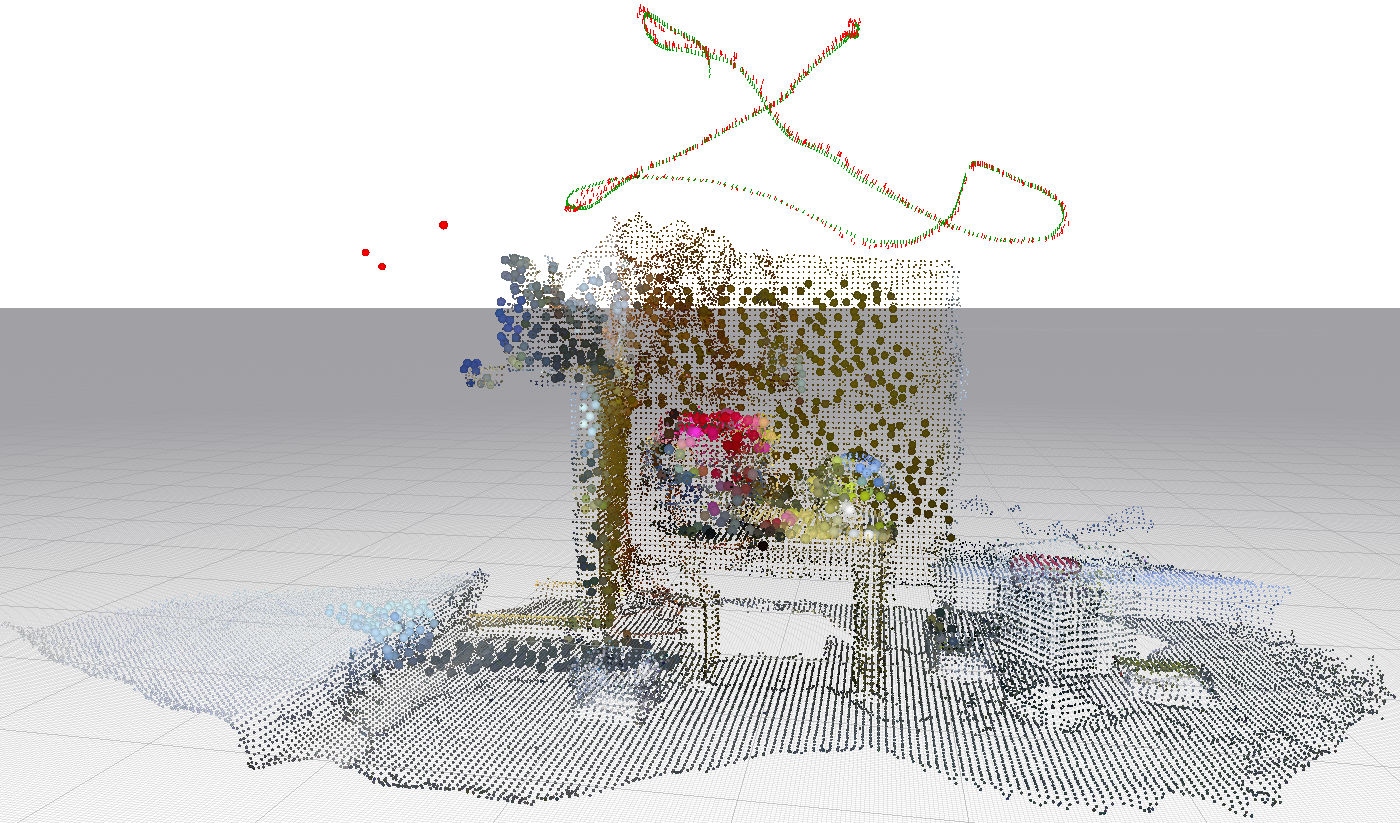
\includegraphics[width=0.45\textwidth]{localization-system-evaluation/tests-6dof/kinect-fly-30cm-per-sec-velocity/drl}
%	\caption{Example of filtered point cloud from Kinect data (grid with 0.5 m spacing)}
%	\label{fig:localization-system-evaluation_kinect-fly-30cm-per-sec-velocity-drl-filters}
%\end{figure}



\subsection{Point cloud registration}

Looking at \Cref{tab:localization-system-evaluation_6-dof-results} and \crefrange{fig:localization-system-evaluation_kinect-fly-30cm-per-sec-velocity-drl-cumulative}{fig:localization-system-evaluation_kinect-translations-robot-movement-path-combined-3d}, it is clear that the \gls{drl} system is able to register point clouds with high accuracy, even when they are severely down-sampled (due to real-time processing constraints). Moreover, the localization system is robust against temporary absence of sensor data (when the field of view of the Kinect was outside the known map in the rotations tests) and was able to quickly recover to accurate tracking when valid sensor data was given (analyzing \crefrange{fig:localization-system-evaluation_kinect-rotations-robot-movement-path-combined-xy}{fig:localization-system-evaluation_kinect-translations-robot-movement-path-combined-3d} it can be seen that the ethzasl\_icp\_mapper was less successful in detecting unreliable pose estimations and recovering from then). In these situations the recovery algorithms were activated, switching the registration algorithm from \gls{icp} point-to-point to \gls{icp} point-to-plane (89 times in 541 registrations in the case of the rotations tests and 0 on the remaining two tests). Given that these sensor data outages were temporary, the initial pose algorithms weren't necessary. Nevertheless, if the Kinect remained outside the map for a longer period of time, the localization system would alert that the tracking was lost and it would try to find its current pose using feature matching.

\begin{figure}[H]
	\centering
	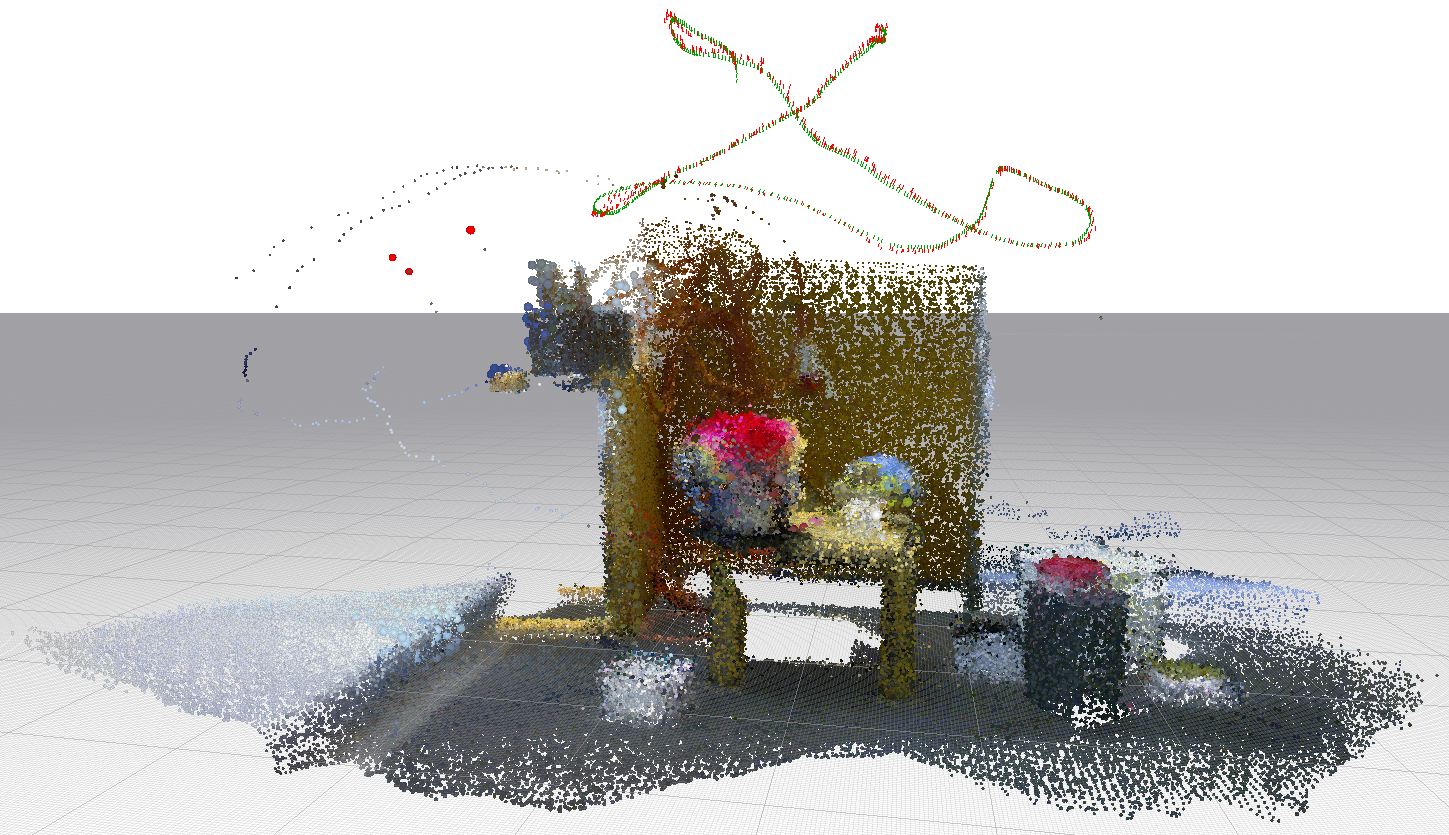
\includegraphics[width=0.33\textwidth]{localization-system-evaluation/tests-6dof/kinect-fly-30cm-per-sec-velocity/drl-cumulative}
	\caption{Point clouds assembled on top of the map using the DRL poses (for the top part of the figure: green arrows $\rightarrow$ ground truth poses, red arrows $\rightarrow$ DRL poses)}
	\label{fig:localization-system-evaluation_kinect-fly-30cm-per-sec-velocity-drl-cumulative}
\end{figure}

\begin{figure}[H]
	\centering
	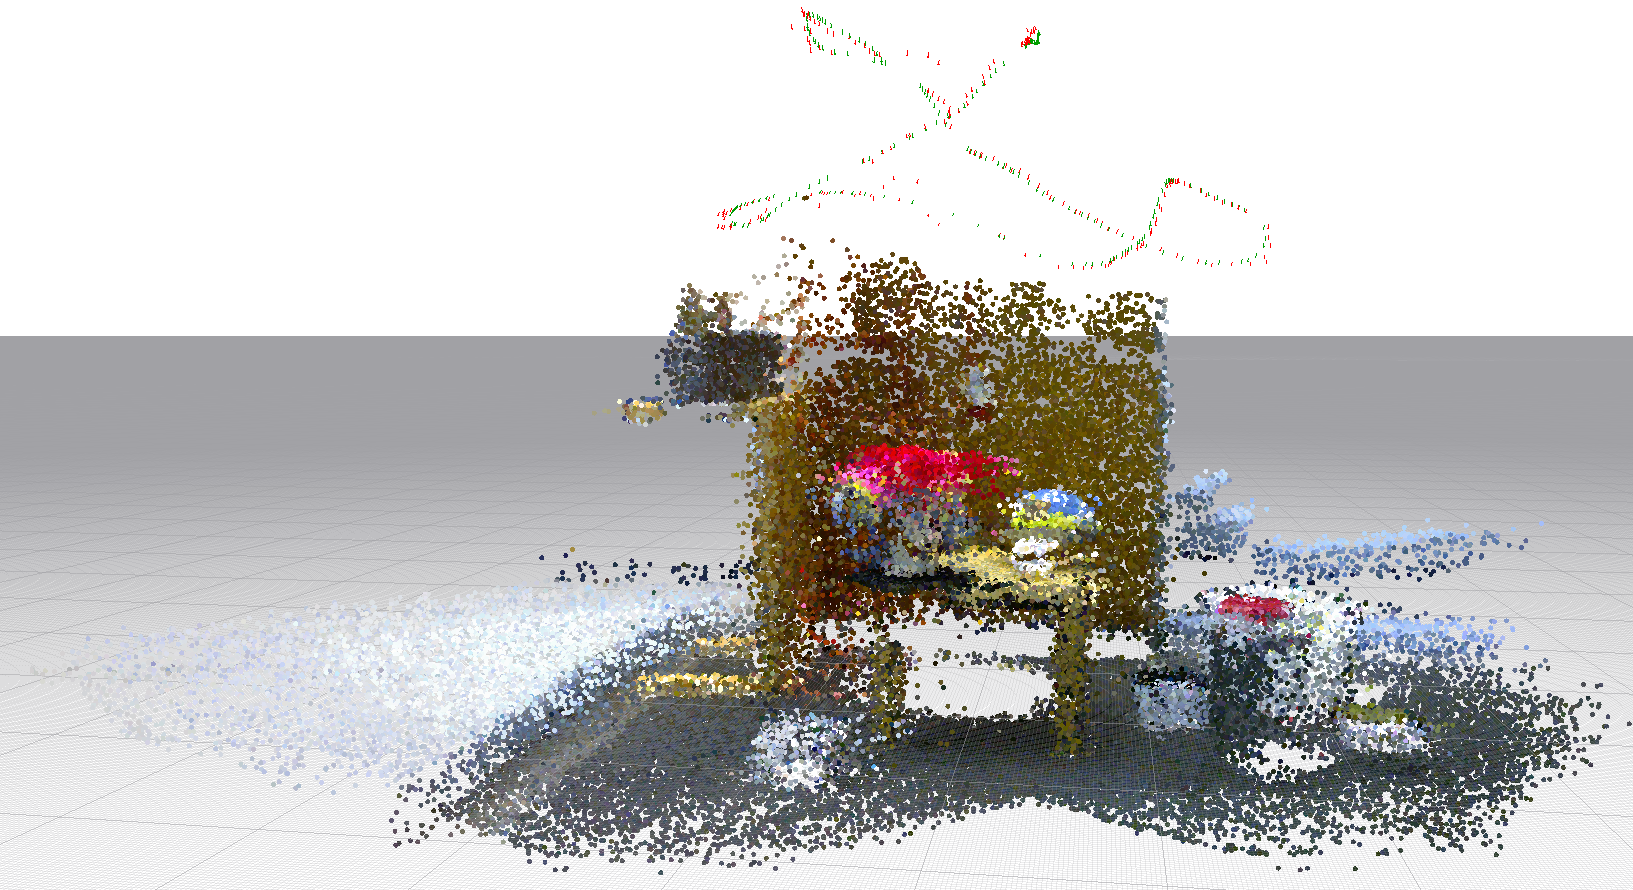
\includegraphics[width=0.33\textwidth]{localization-system-evaluation/tests-6dof/kinect-fly-30cm-per-sec-velocity/ethzasl-icp-mapping-cumulative}
	\caption{Point clouds assembled on top of the map using the ethzasl\_icp\_mapper poses (for the top part of the figure: green arrows $\rightarrow$ ground truth poses, red arrows $\rightarrow$ ethzasl\_icp\_mapper poses)}
	\label{fig:localization-system-evaluation_kinect-fly-30cm-per-sec-velocity-ethzasl-icp-mapping-cumulative}
\end{figure}

\begin{figure}[H]
	\centering
	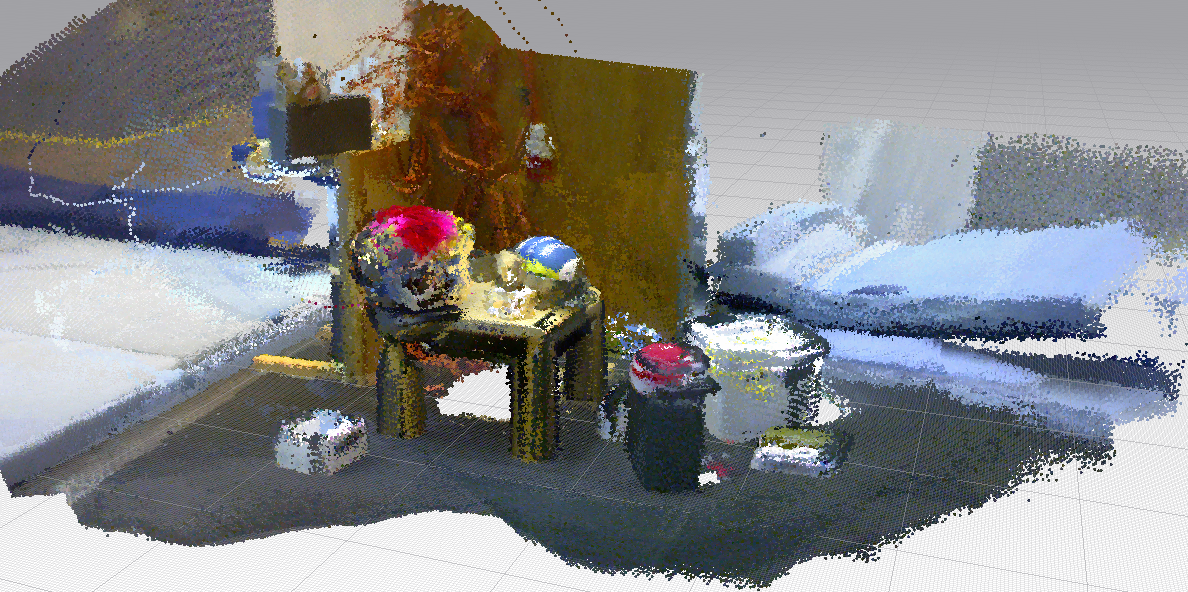
\includegraphics[width=0.33\textwidth]{localization-system-evaluation/tests-6dof/kinect-fly-30cm-per-sec-velocity/ground-truth-cumulative}
	\caption{Point clouds assembled on top of the map using the ground truth poses}
	\label{fig:localization-system-evaluation_kinect-fly-30cm-per-sec-velocity-gt-cumulative}
\end{figure}


\begin{figure}[H]
	\centering
	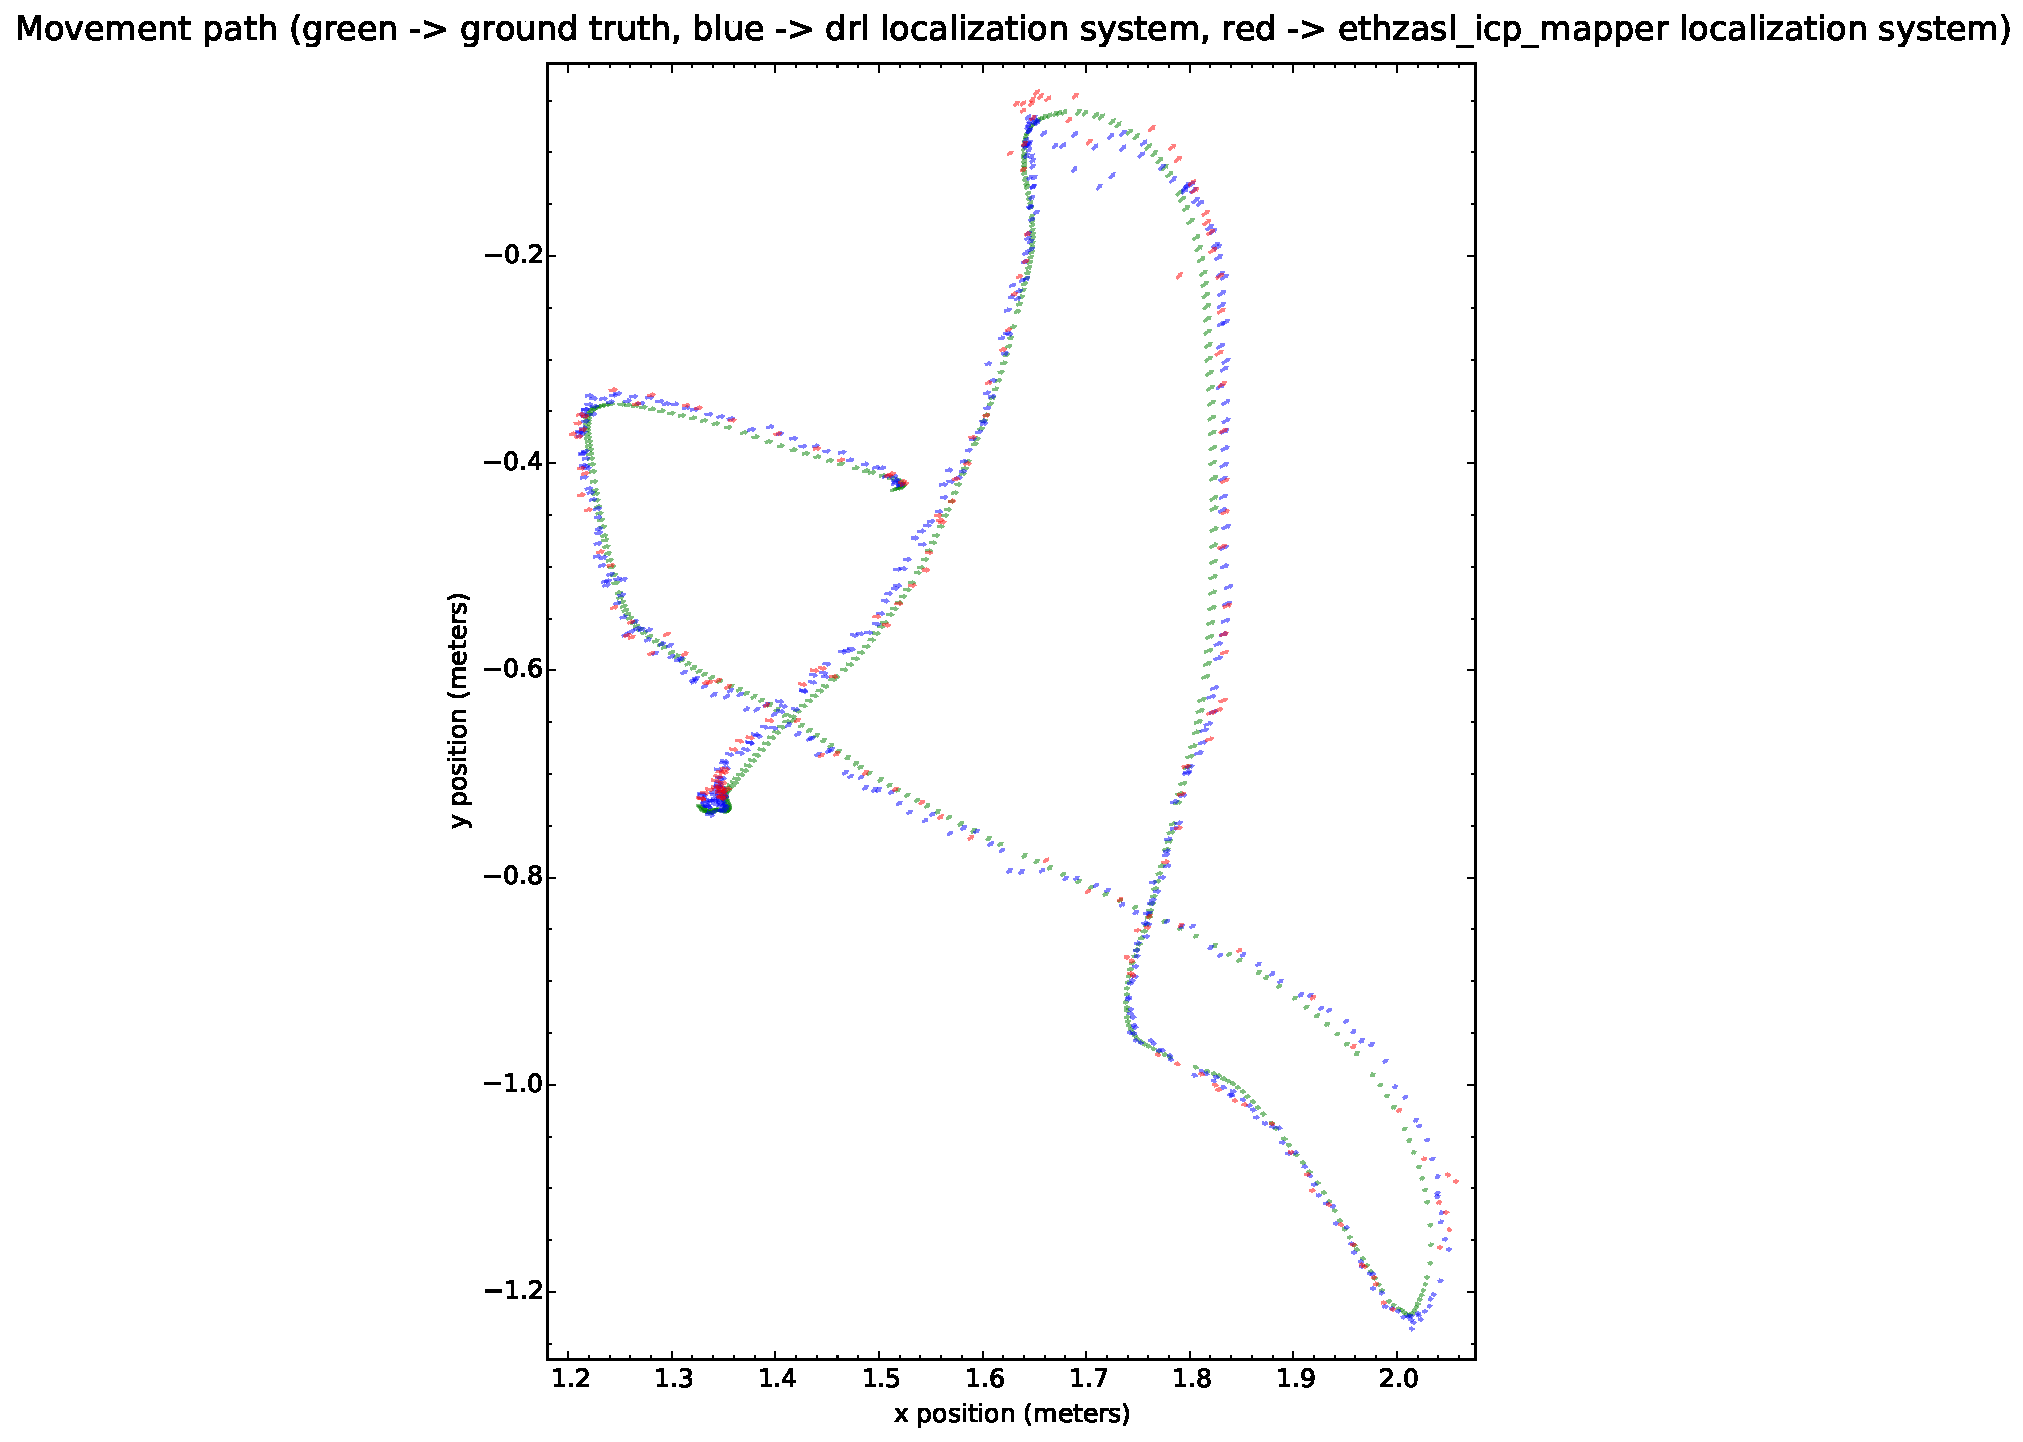
\includegraphics[width=0.3\textwidth]{localization-system-evaluation/tests-6dof/kinect-fly-30cm-per-sec-velocity/robot-movement-path-combined-xy}
	\caption{2D plot XY Poses estimated in the 6 DoF fly test by the ground truth (green) and DRL (blue) and ethzasl\_icp\_mapper (red)}
	\label{fig:localization-system-evaluation_kinect-fly-robot-movement-path-combined-xy}
\end{figure}

\begin{figure}[H]
	\centering
	\hspace*{0.25cm}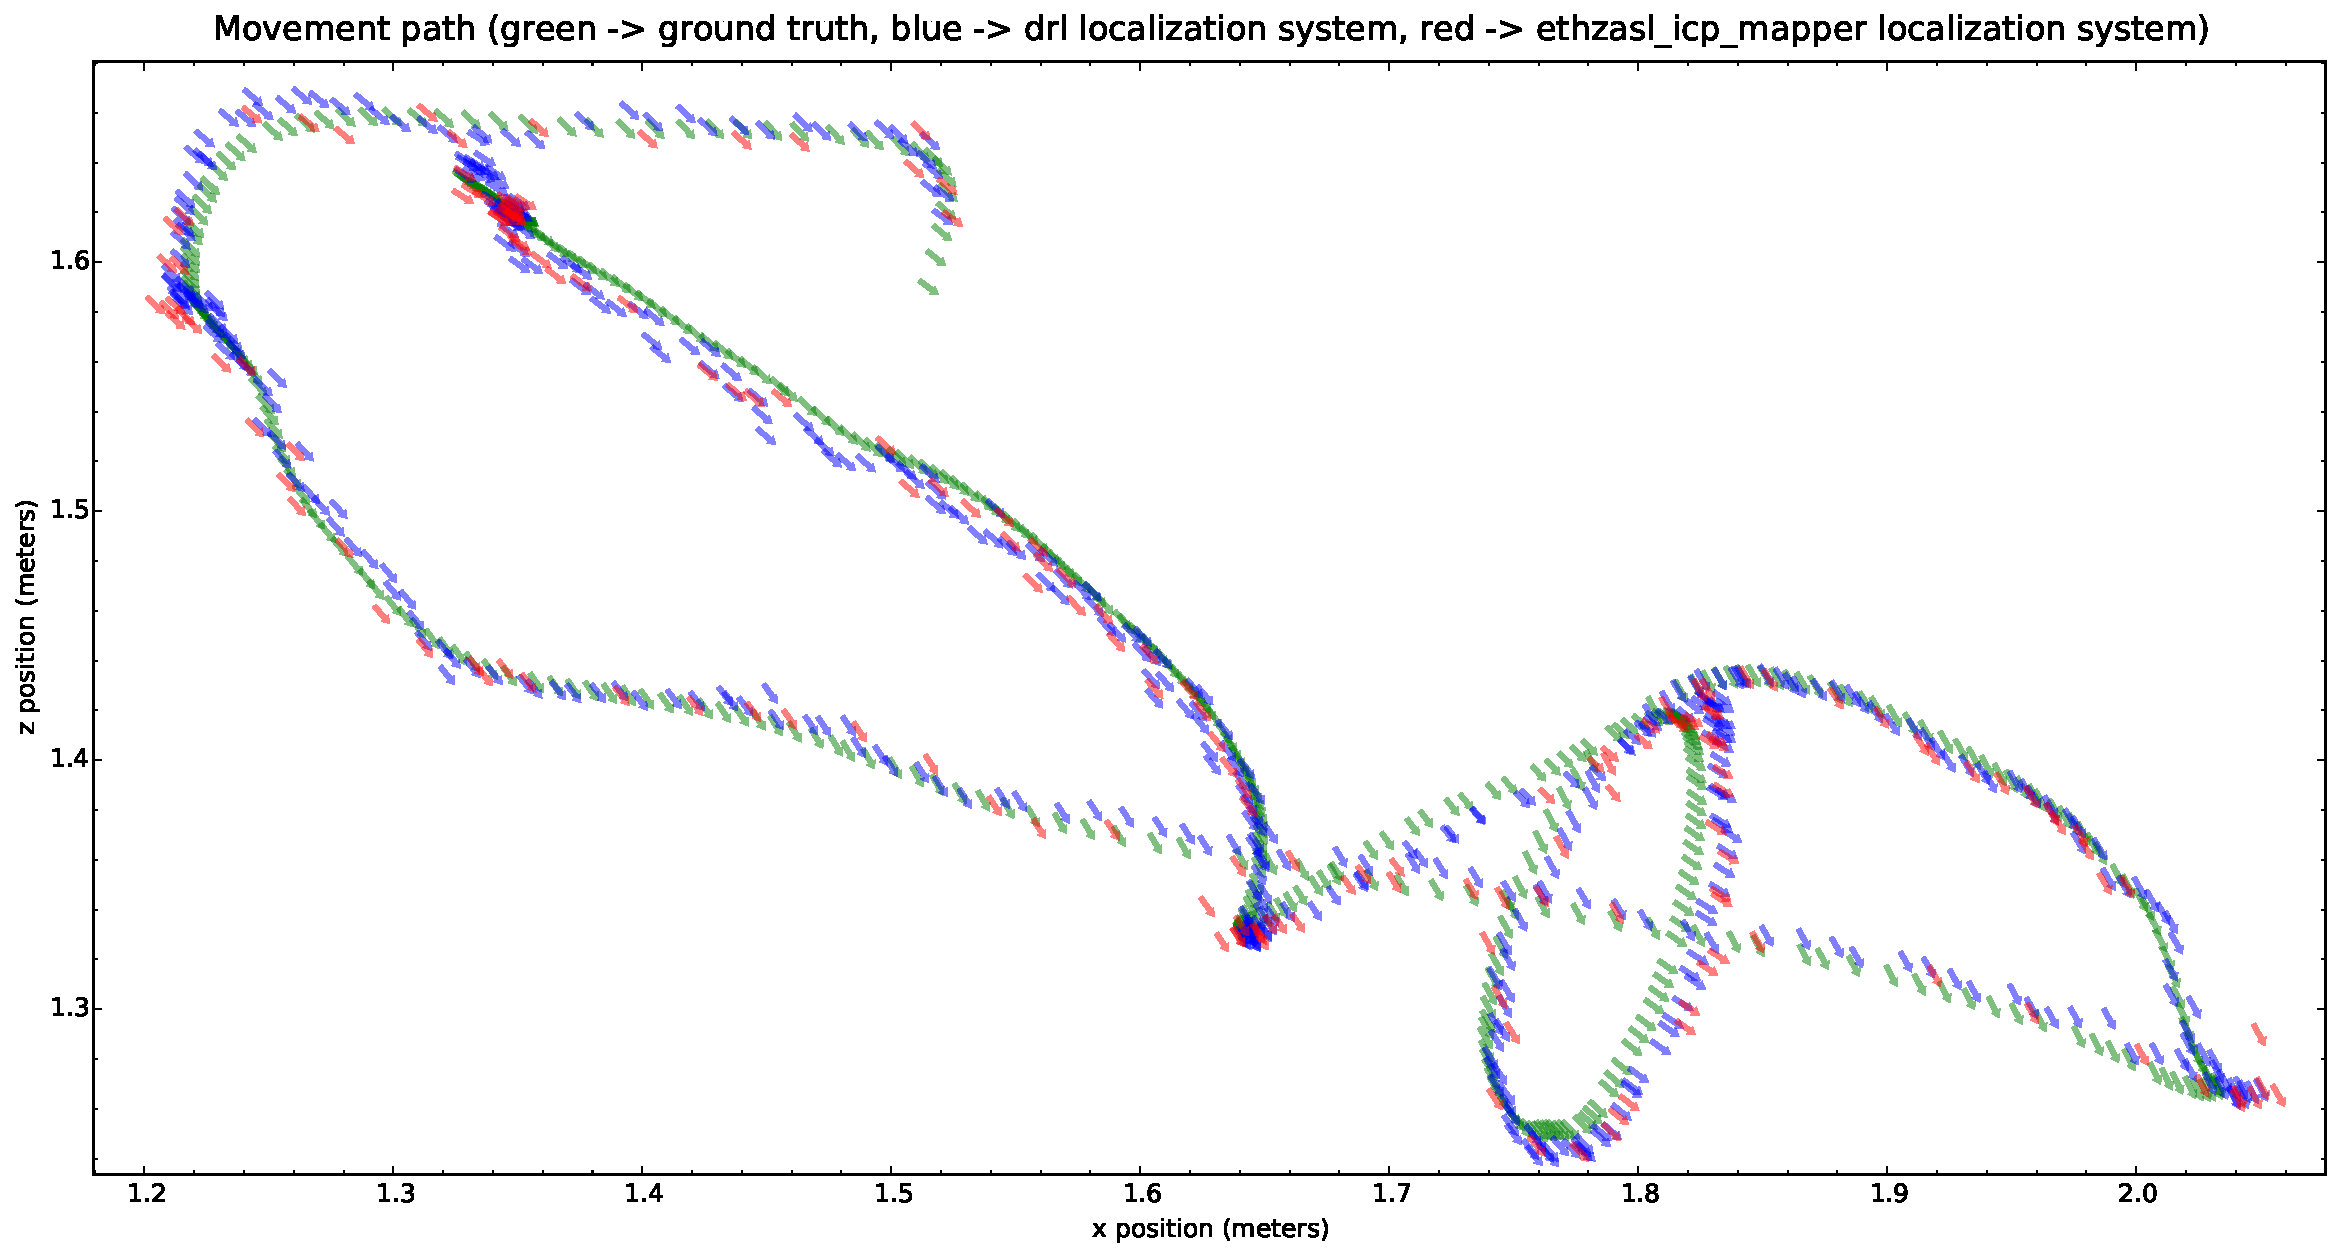
\includegraphics[width=0.28\textwidth]{localization-system-evaluation/tests-6dof/kinect-fly-30cm-per-sec-velocity/robot-movement-path-combined-xz}
	\caption{2D plot XZ Poses estimated in the 6 DoF fly test by the ground truth (green) and DRL (blue) and ethzasl\_icp\_mapper (red)}
	\label{fig:localization-system-evaluation_kinect-fly-robot-movement-path-combined-xz}
\end{figure}

\begin{figure}[H]
	\centering
	\includegraphics[trim={2.5cm 0 0 1.5cm}, clip, width=0.49\textwidth]{localization-system-evaluation/tests-6dof/kinect-fly-30cm-per-sec-velocity/robot-movement-path-combined-3d}
	\caption{3D plot XYZ Poses estimated in the 6 DoF fly test by the ground truth (green) and DRL (blue) and ethzasl\_icp\_mapper (red)}
	\label{fig:localization-system-evaluation_kinect-fly-robot-movement-path-combined-3d}
\end{figure}


\begin{figure}[H]
	\centering
	\includegraphics[width=0.355\textwidth]{localization-system-evaluation/tests-6dof/kinect-rotations-10cm-per-sec-velocity/robot-movement-path-combined-xy}
	\caption{2D plot XY Poses estimated in the 6 DoF rotations test by the ground truth (green) and DRL (blue) and ethzasl\_icp\_mapper (red)}
	\label{fig:localization-system-evaluation_kinect-rotations-robot-movement-path-combined-xy}
\end{figure}

\begin{figure}[H]
	\centering
	\hspace*{0.25cm}\includegraphics[width=0.34\textwidth]{localization-system-evaluation/tests-6dof/kinect-rotations-10cm-per-sec-velocity/robot-movement-path-combined-xz}
	\caption{2D plot XZ Poses estimated in the 6 DoF rotations test by the ground truth (green) and DRL (blue) and ethzasl\_icp\_mapper (red)}
	\label{fig:localization-system-evaluation_kinect-rotations-robot-movement-path-combined-xz}
\end{figure}

\begin{figure}[H]
	\centering
	\includegraphics[trim={2.5cm 0 0 1.5cm}, clip, width=0.47\textwidth]{localization-system-evaluation/tests-6dof/kinect-rotations-10cm-per-sec-velocity/robot-movement-path-combined-3d}
	\caption{3D plot XYZ Poses estimated in the 6 DoF rotations test by the ground truth (green) and DRL (blue) and ethzasl\_icp\_mapper (red)}
	\label{fig:localization-system-evaluation_kinect-rotations-robot-movement-path-combined-3d}
\end{figure}


\begin{figure}[H]
	\centering
	\includegraphics[width=0.27\textwidth]{localization-system-evaluation/tests-6dof/kinect-translations-20cm-per-sec-velocity/robot-movement-path-combined-xy}
	\caption{2D plot XY Poses estimated in the 6 DoF translations test by the ground truth (green) and DRL (blue) and ethzasl\_icp\_mapper (red)}
	\label{fig:localization-system-evaluation_kinect-translations-robot-movement-path-combined-xy}
\end{figure}

\begin{figure}[H]
	\centering
	\hspace*{0.25cm}\includegraphics[width=0.26\textwidth]{localization-system-evaluation/tests-6dof/kinect-translations-20cm-per-sec-velocity/robot-movement-path-combined-xz}
	\caption{2D plot XZ Poses estimated in the 6 DoF translations test by the ground truth (green) and DRL (blue) and ethzasl\_icp\_mapper (red)}
	\label{fig:localization-system-evaluation_kinect-translations-robot-movement-path-combined-xz}
\end{figure}

\begin{figure}[H]
	\centering
	\includegraphics[trim={2.5cm 0 0 1.5cm}, clip, width=0.42\textwidth]{localization-system-evaluation/tests-6dof/kinect-translations-20cm-per-sec-velocity/robot-movement-path-combined-3d}
	\caption{3D plot XYZ Poses estimated in the 6 DoF translations test by the ground truth (green) and DRL (blue) and ethzasl\_icp\_mapper (red)}
	\label{fig:localization-system-evaluation_kinect-translations-robot-movement-path-combined-3d}
\end{figure}

\subsection{Translation and rotation errors}

The results presented in \Cref{tab:localization-system-evaluation_6-dof-results} and in \cref{fig:localization-system-evaluation_kinect-fly-30cm-per-sec-velocity-translation-error,fig:localization-system-evaluation_kinect-fly-30cm-per-sec-velocity-rotation-error-asl}, shown that the localization system can maintain high accuracy pose tracking, with translation error below two centimeters and rotation error around 3 degrees when good sensor data is available. Moreover it can quickly recover from temporary registration problems caused by occlusions or accelerations.

Analyzing the results in \Cref{tab:localization-system-evaluation_6-dof-results} and in \crefrange{fig:localization-system-evaluation_kinect-fly-30cm-per-sec-velocity-drl-cumulative}{fig:localization-system-evaluation_kinect-translations-robot-movement-path-combined-3d}, it can also be concluded that the \gls{drl} system achieved better pose tracking than the \emph{ethzasl\_icp\_mapper} \gls{ros} package (17.9 mm vs 22.8 mm of translation error and 3.0º vs 3.5º of rotation error), while achieving more than double of the refresh rate in the fly test. For the translations test the \gls{drl} system achieved better tracking in relation to the fly test ()




\begin{figure}[H]
	\centering
	\includegraphics[trim={0 0 0 1cm}, clip, width=0.47\textwidth]{localization-system-evaluation/tests-6dof/kinect-fly-30cm-per-sec-velocity/translation-error-millimeters-distributions}
	\caption{Probability distributions for the DRL translation errors in the 6 DoF fly test}
	\label{fig:localization-system-evaluation_kinect-fly-30cm-per-sec-velocity-translation-error}
\end{figure}

\begin{figure}[H]
	\centering
-	\includegraphics[trim={0 0 0 1cm}, clip, width=0.47\textwidth]{localization-system-evaluation/tests-6dof/kinect-fly-30cm-per-sec-velocity/rotation-error-degrees-distributions}
	\caption{Probability distributions for the DRL rotation errors in the 6 DoF fly test}
	\label{fig:localization-system-evaluation_kinect-fly-30cm-per-sec-velocity-rotation-error}
\end{figure}

\begin{figure}[H]
	\centering
	\includegraphics[trim={0 0 0 1cm}, clip, width=0.47\textwidth]{localization-system-evaluation/tests-6dof/kinect-fly-30cm-per-sec-velocity/ethzasl-translation-error-millimeters-distributions}
	\caption{Probability distributions for the ethzasl\_icp\_mapper translation errors in the 6 DoF fly test}
	\label{fig:localization-system-evaluation_kinect-fly-30cm-per-sec-velocity-translation-error-asl}
\end{figure}

\begin{figure}[H]
	\centering
	\includegraphics[trim={0 0 0 1cm}, clip, width=0.47\textwidth]{localization-system-evaluation/tests-6dof/kinect-fly-30cm-per-sec-velocity/ethzasl-rotation-error-degrees-distributions}
	\caption{Probability distributions for the ethzasl\_icp\_mapper rotation errors in the 6 DoF fly test}
	\label{fig:localization-system-evaluation_kinect-fly-30cm-per-sec-velocity-rotation-error-asl}
\end{figure}


%\begin{figure}[H]
%	\centering
%	\includegraphics[width=0.4\textwidth]{localization-system-evaluation/tests-6dof/kinect-rotations-10cm-per-sec-velocity/translation-error-millimeters-distributions}
%	\caption{Probability distributions for the DRL translation errors in the 6 DoF rotations test}
%	\label{fig:localization-system-evaluation_kinect-rotations-10cm-per-sec-velocity-translation-error}
%\end{figure}
%
%\begin{figure}[H]
%	\centering
%	\includegraphics[width=0.4\textwidth]{localization-system-evaluation/tests-6dof/kinect-rotations-10cm-per-sec-velocity/rotation-error-degrees-distributions}
%	\caption{Probability distributions for the DRL rotation errors in the 6 DoF rotations test}
%	\label{fig:localization-system-evaluation_kinect-rotations-10cm-per-sec-velocity-rotation-error}
%\end{figure}
%
%\begin{figure}[H]
%	\centering
%	\includegraphics[width=0.4\textwidth]{localization-system-evaluation/tests-6dof/kinect-rotations-10cm-per-sec-velocity/ethzasl-translation-error-millimeters-distributions}
%	\caption{Probability distributions for the ethzasl\_icp\_mapper translation errors in the 6 DoF rotations test}
%	\label{fig:localization-system-evaluation_kinect-rotations-10cm-per-sec-velocity-translation-error-asl}
%\end{figure}
%
%\begin{figure}[H]
%	\centering
%	\includegraphics[width=0.4\textwidth]{localization-system-evaluation/tests-6dof/kinect-rotations-10cm-per-sec-velocity/ethzasl-rotation-error-degrees-distributions}
%	\caption{Probability distributions for the ethzasl\_icp\_mapper rotation errors in the 6 DoF rotations test}
%	\label{fig:localization-system-evaluation_kinect-rotations-10cm-per-sec-velocity-rotation-error-asl}
%\end{figure}
%
%
%\begin{figure}[H]
%	\centering
%	\includegraphics[width=0.4\textwidth]{localization-system-evaluation/tests-6dof/kinect-translations-20cm-per-sec-velocity/translation-error-millimeters-distributions}
%	\caption{Probability distributions for the DRL translation errors in the 6 DoF translations test}
%	\label{fig:localization-system-evaluation_kinect-translations-20cm-per-sec-velocity-translation-error}
%\end{figure}
%
%\begin{figure}[H]
%	\centering
%	\includegraphics[width=0.4\textwidth]{localization-system-evaluation/tests-6dof/kinect-translations-20cm-per-sec-velocity/rotation-error-degrees-distributions}
%	\caption{Probability distributions for the DRL rotation errors in the 6 DoF translations test}
%	\label{fig:localization-system-evaluation_kinect-translations-20cm-per-sec-velocity-rotation-error}
%\end{figure}
%
%\begin{figure}[H]
%	\centering
%	\includegraphics[width=0.4\textwidth]{localization-system-evaluation/tests-6dof/kinect-translations-20cm-per-sec-velocity/ethzasl-translation-error-millimeters-distributions}
%	\caption{Probability distributions for the ethzasl\_icp\_mapper translation errors in the 6 DoF translations test}
%	\label{fig:localization-system-evaluation_kinect-translations-20cm-per-sec-velocity-translation-error-asl}
%\end{figure}
%
%\begin{figure}[H]
%	\centering
%	\includegraphics[width=0.4\textwidth]{localization-system-evaluation/tests-6dof/kinect-translations-20cm-per-sec-velocity/ethzasl-rotation-error-degrees-distributions}
%	\caption{Probability distributions for the ethzasl\_icp\_mapper rotation errors in the 6 DoF translations test}
%	\label{fig:localization-system-evaluation_kinect-translations-20cm-per-sec-velocity-rotation-error-asl}
%\end{figure}



\subsection{Computation time}

The localization system was able to achieve a mean computation time low enough to allow real time processing of the Kinect point cloud sensor data (shown in \Cref{fig:localization-system-evaluation_kinect-fly-30cm-per-sec-velocity-computation-time}). Depending on the accuracy requirements, the computation time can be lowered even further by tuning the preprocessing filters, in order to reduce the number of points used in the cloud registration.

Comparing \Cref{fig:localization-system-evaluation_kinect-fly-30cm-per-sec-velocity-computation-time} with \Cref{fig:localization-system-evaluation_kinect-fly-30cm-per-sec-velocity-computation-time-asl} it can also be seen that the \gls{drl} system required about ten times less processing time in relation to the \emph{ethzasl\_icp\_mapper} system.


\begin{figure}[H]
	\centering
	\includegraphics[trim={0 0 0 1cm}, clip, width=0.47\textwidth]{localization-system-evaluation/tests-6dof/kinect-fly-30cm-per-sec-velocity/computation-times-milliseconds-global-time-distributions}
	\caption{Probability distributions for the DRL global computation time in the 6 DoF translations test}
	\label{fig:localization-system-evaluation_kinect-fly-30cm-per-sec-velocity-computation-time}
\end{figure}

\begin{figure}[H]
	\centering
	\includegraphics[trim={0 0 0 1cm}, clip, width=0.47\textwidth]{localization-system-evaluation/tests-6dof/kinect-fly-30cm-per-sec-velocity/ethzasl-computation-times-milliseconds-global-time-distributions}
	\caption{Probability distributions for the ethzasl\_icp\_mapper global computation time in the 6 DoF translations test}
	\label{fig:localization-system-evaluation_kinect-fly-30cm-per-sec-velocity-computation-time-asl}
\end{figure}


%\begin{figure}[H]
%	\centering
%	\includegraphics[width=0.45\textwidth]{localization-system-evaluation/tests-6dof/kinect-rotations-10cm-per-sec-velocity/computation-times-milliseconds-global-time-distributions}
%	\caption{Probability distributions for the DRL global computation time in the 6 DoF rotations test}
%	\label{fig:localization-system-evaluation_kinect-rotations-10cm-per-sec-velocity-computation-time}
%\end{figure}
%
%\begin{figure}[H]
%	\centering
%	\includegraphics[width=0.45\textwidth]{localization-system-evaluation/tests-6dof/kinect-rotations-10cm-per-sec-velocity/ethzasl-computation-times-milliseconds-global-time-distributions}
%	\caption{Probability distributions for the ethzasl\_icp\_mapper global computation time in the 6 DoF rotations test}
%	\label{fig:localization-system-evaluation_kinect-rotations-10cm-per-sec-velocity-computation-time-asl}
%\end{figure}
%
%
%\begin{figure}[H]
%	\centering
%	\includegraphics[width=0.45\textwidth]{localization-system-evaluation/tests-6dof/kinect-translations-20cm-per-sec-velocity/computation-times-milliseconds-global-time-distributions}
%	\caption{Probability distributions for the DRL global computation time in the 6 DoF translations test}
%	\label{fig:localization-system-evaluation_kinect-translations-20cm-per-sec-velocity-computation-time}
%\end{figure}
%
%\begin{figure}[H]
%	\centering
%	\includegraphics[width=0.45\textwidth]{localization-system-evaluation/tests-6dof/kinect-translations-20cm-per-sec-velocity/ethzasl-computation-times-milliseconds-global-time-distributions}
%	\caption{Probability distributions for the ethzasl\_icp\_mapper global computation time in the 6 DoF translations test}
%	\label{fig:localization-system-evaluation_kinect-translations-20cm-per-sec-velocity-computation-time-asl}
%\end{figure}

\subsection{Mapping}

The \gls{drl} system can perform mapping of the environment and is able to build very detailed point clouds. These point clouds can be continuously re-sampled with the Moving Least Squares algorithm (example in \Cref{fig:localization-system-evaluation_kinect-fly-30cm-per-sec-velocity-drl-slam}) in order to reconstruct the surfaces of the environment and attenuate the double wall effects and high sensor noise.

Besides the internal mapping capabilities of the \gls{drl} system, it can also be paired with the OctoMap \cite{Hornung2013} library in order to perform probabilistic integration of sensor data and be able to remove missing objects from the reference point cloud.


\begin{figure}[H]
	\centering
	\begin{subfigure}[ht]{0.4\textwidth}
		\centering
		\includegraphics[width=\textwidth]{localization-system-evaluation/tests-6dof/kinect-fly-30cm-per-sec-velocity/3d-slam-1-gt}
	\end{subfigure}
	\begin{subfigure}[ht]{0.4\textwidth}
		\centering
		\includegraphics[width=\textwidth]{localization-system-evaluation/tests-6dof/kinect-fly-30cm-per-sec-velocity/3d-slam-2-gt}
	\end{subfigure}
%	\begin{subfigure}[ht]{0.4\textwidth}
%		\centering
%		\includegraphics[width=\textwidth]{localization-system-evaluation/tests-6dof/kinect-fly-30cm-per-sec-velocity/3d-slam-3-gt}
%	\end{subfigure}
	\begin{subfigure}[ht]{0.4\textwidth}
		\centering
		\includegraphics[width=\textwidth]{localization-system-evaluation/tests-6dof/kinect-fly-30cm-per-sec-velocity/3d-slam-4-gt}
	\end{subfigure}
	\caption{3D SLAM using the ground truth poses}
	\label{fig:localization-system-evaluation_kinect-fly-30cm-per-sec-velocity-gt-slam}
\end{figure}


\begin{figure}[H]
	\centering
	\begin{subfigure}[ht]{0.45\textwidth}
		\centering
		\includegraphics[width=\textwidth]{localization-system-evaluation/tests-6dof/kinect-fly-30cm-per-sec-velocity/3d-slam-1}
	\end{subfigure}
	\begin{subfigure}[ht]{0.45\textwidth}
		\centering
		\includegraphics[width=\textwidth]{localization-system-evaluation/tests-6dof/kinect-fly-30cm-per-sec-velocity/3d-slam-2}
	\end{subfigure}
%	\begin{subfigure}[ht]{0.45\textwidth}
%		\centering
%		\includegraphics[width=\textwidth]{localization-system-evaluation/tests-6dof/kinect-fly-30cm-per-sec-velocity/3d-slam-3}
%	\end{subfigure}
	\begin{subfigure}[ht]{0.45\textwidth}
		\centering
		\includegraphics[width=\textwidth]{localization-system-evaluation/tests-6dof/kinect-fly-30cm-per-sec-velocity/3d-slam-4}
	\end{subfigure}
	\caption{3D SLAM using the localization system with surface reconstruction}
	\label{fig:localization-system-evaluation_kinect-fly-30cm-per-sec-velocity-drl-slam}
\end{figure}

\section{Conclusions}\label{sec:conclusions}

The proposed localization system is able to maintain pose tracking with less than 1-2 centimeters of translation error and less than a 1-3 degrees of rotation error (in 3 and 6 DoF respectively) with the robot / sensors moving at several velocities even in cluttered and dynamic environments. Moreover, when tracking is lost or no initial pose is given, the system is able to find a valid global pose estimate by switching to more robust registration algorithms that use feature matching. This approach achieved fast and accurate pose estimation with robust tracking recovery and reliable initial pose estimation while also providing the set of the accepted initial poses before registration refinement, which can be very valuable information for a navigation supervisor when the robot is in an ambiguous region that can be registered in similar zones of the known map. The system also allows dynamic reconfiguration of the number of laser scans to assemble in order to mitigate laser measurement errors and can adapt its rate of operation according to the robot estimated velocity.

The sub-centimeter accuracy achieved by the proposed localization system along with the selective map update capability (using partial or full sensor data integration) and the need of no artificial landmarks / ambient modifications will allow the fast deployment of mobile robots capable to operate safely and accurately in cluttered environments.

\section*{Acknowledgments}

The authors would like to thank everyone involved in the CARLoS Project. This project has received funding from the European Commission Seventh Framework Programme for Research and Technological Development under the grant agreement number 606363, and from the national project "NORTE-07-0124-FEDER-000060".



%---------------------------------------------------------------------------------------------------
% Bibliography
%---------------------------------------------------------------------------------------------------

\section*{References}

\bibliographystyle{elsarticle-harv}
\bibliography{references/references}


\end{document}
